%% For double-blind review submission, w/o CCS and ACM Reference (max submission space)
\documentclass[sigplan,10pt,review,anonymous]{acmart}
\settopmatter{printfolios=true,printccs=false,printacmref=false}
%% For double-blind review submission, w/ CCS and ACM Reference
%\documentclass[sigplan,review,anonymous]{acmart}\settopmatter{printfolios=true}
%% For single-blind review submission, w/o CCS and ACM Reference (max submission space)
%\documentclass[sigplan,review]{acmart}\settopmatter{printfolios=true,printccs=false,printacmref=false}
%% For single-blind review submission, w/ CCS and ACM Reference
%\documentclass[sigplan,review]{acmart}\settopmatter{printfolios=true}
%% For final camera-ready submission, w/ required CCS and ACM Reference
%\documentclass[sigplan]{acmart}\settopmatter{}


%% Conference information
%% Supplied to authors by publisher for camera-ready submission;
%% use defaults for review submission.
\acmConference[PL'22]{ACM SIGPLAN Conference on Programming Languages}{January 01--03, 2022}{New York, NY, USA}
%\acmConference{}{}{}
\acmYear{2022}
\acmISBN{} % \acmISBN{978-x-xxxx-xxxx-x/YY/MM}
\acmDOI{} % \acmDOI{10.1145/nnnnnnn.nnnnnnn}
\startPage{1}

%% Copyright information
%% Supplied to authors (based on authors' rights management selection;
%% see authors.acm.org) by publisher for camera-ready submission;
%% use 'none' for review submission.
\setcopyright{none}
%\setcopyright{acmcopyright}
%\setcopyright{acmlicensed}
%\setcopyright{rightsretained}
%\copyrightyear{2018}           %% If different from \acmYear

%% Bibliography style
\bibliographystyle{ACM-Reference-Format}
%% Citation style
%\citestyle{acmauthoryear}  %% For author/year citations
%\citestyle{acmnumeric}     %% For numeric citations
%\setcitestyle{nosort}      %% With 'acmnumeric', to disable automatic
                            %% sorting of references within a single citation;
                            %% e.g., \cite{Smith99,Carpenter05,Baker12}
                            %% rendered as [14,5,2] rather than [2,5,14].
%\setcitesyle{nocompress}   %% With 'acmnumeric', to disable automatic
                            %% compression of sequential references within a
                            %% single citation;
                            %% e.g., \cite{Baker12,Baker14,Baker16}
                            %% rendered as [2,3,4] rather than [2-4].


%%%%%%%%%%%%%%%%%%%%%%%%%%%%%%%%%%%%%%%%%%%%%%%%%%%%%%%%%%%%%%%%%%%%%%
%% Note: Authors migrating a paper from traditional SIGPLAN
%% proceedings format to PACMPL format must update the
%% '\documentclass' and topmatter commands above; see
%% 'acmart-pacmpl-template.tex'.
%%%%%%%%%%%%%%%%%%%%%%%%%%%%%%%%%%%%%%%%%%%%%%%%%%%%%%%%%%%%%%%%%%%%%%


%% Some recommended packages.
\usepackage{booktabs}   %% For formal tables:
                        %% http://ctan.org/pkg/booktabs
\usepackage{subcaption} %% For complex figures with subfigures/subcaptions
                        %% http://ctan.org/pkg/subcaption

\usepackage{titlesec,balance}

\usepackage{eufrak}
%\usepackage{unicode-math}
\usepackage{mathrsfs}

\setcounter{secnumdepth}{4}
%\renewcommand{\theparagraph}{\textit{(\alph{paragraph})}}
%\renewcommand{\theparagraph}{\arabic{paragraph}}
\titleformat{\paragraph}[runin]
{\normalfont\normalsize\bfseries}{\theparagraph}{1em}{}
\titlespacing*{\paragraph}
{0pt}{1.5ex plus 1ex minus .2ex}{1.5ex plus .2ex}

\usepackage{mdframed}

% package area
\usepackage{extarrows}
\usepackage{xspace,enumitem}
\usepackage{cleveref}
\usepackage{listings}
\usepackage{adjustbox}
\usepackage{multirow}
\usepackage{marvosym}
\let\Cross\relax
\usepackage{bbding}
\usepackage{color}
\usepackage{relsize}
\usepackage{xifthen}% provides \ifthenelse and \isempty
\usepackage{tikz}
\usetikzlibrary{shapes.multipart}
\usetikzlibrary{automata, positioning, arrows}
\tikzset{
->, % makes the edges directed
>=latex, % makes the arrow heads bold
node distance=3cm, % specifies the minimum distance between two nodes. Change if necessary.
every state/.style={thick, fill=red!10}, % sets the properties for each ’state’ node
%initial text=$ $, % sets the text that appears on the start arrow
auto,
}

\usetikzlibrary{calc,decorations.pathmorphing,shapes}

\newcounter{sarrow}
\newcommand\xrsquigarrow[1]{%
\stepcounter{sarrow}%
\mathrel{\begin{tikzpicture}[baseline= {( $ (current bounding box.south) + (0,-0.5ex) $ )}]
\node[inner sep=.5ex] (\thesarrow) {$\scriptstyle #1$};
\path[draw,<-,decorate,
  decoration={zigzag,amplitude=0.7pt,segment length=1.2mm,pre=lineto,pre length=4pt}] 
    (\thesarrow.south east) -- (\thesarrow.south west);
\end{tikzpicture}}%
}

%lstlisting settings
\lstset{%
  % backgroundcolor=\color{white},
  language=java, 
  basicstyle=\small\ttfamily,
  keywordstyle=\sffamily\bfseries,
  captionpos=none,
  columns=flexible,
  keepspaces=true,
  showspaces=false,               % show spaces adding particular underscores
  showstringspaces=false,         % underline spaces within strings
  showtabs=false,                 % show tabs within strings adding particular underscores
  breaklines=true,                % sets automatic line breaking
  breakatwhitespace=true,         % sets if automatic breaks should only happen at whitespace
  escapeinside={(*}{*)},
  literate={lam}{{$\lambda$}}1 {->}{{$\rightarrow$}}1 {Top}{{$\top$}}1 {o+o}{{$\oplus$}}1 {=>}{{$\Rightarrow$}}1 {/\\}{{$\Lambda$}}1 {forall}{{$\forall$}}1,
  tabsize=2,
  commentstyle=\color{purple}\ttfamily,
  stringstyle=\color{red}\ttfamily,
  sensitive=false,
  aboveskip=2pt,
  belowskip=2pt,
  numbers=left, 
  numbersep=4pt
}

\lstdefinelanguage{java}{
  keywords={int, String, Boolean, static, void, class, extends, this, new, if, then, else, return, Object},
  identifierstyle=\color{black},
  morecomment=[l]{--},
  morecomment=[l]{//},
  morestring=[b]",
  xleftmargin  = 3mm,
  commentstyle=\color{purple}\ttfamily,
  stringstyle=\color{red}\ttfamily,
  morestring=[b]',
  mathescape=true,
  escapeinside={<@}{@>},
}
\def\inline{\lstinline[basicstyle=\ttfamily]}

\renewcommand{\dbltopfraction}{0.9}

% color
\definecolor{carnelian}{rgb}{0.7, 0.11, 0.11}
\newcommand{\ptsrulecolor}{carnelian}

% \newtheorem{theorem}{Theorem}[Section]
% \newtheorem{corollary}{Corollary}[Section]
 \makeatletter 
\renewcommand{\boxed}[1]{\text{\fboxsep=.1em\fbox{\m@th$\displaystyle#1$}}}
% %% rule command
\newcommand{\ruledef}[2]{$\dfrac{\begin{array}[c]{c}#1\end{array}}{\begin{array}[c]{c}#2\end{array}}$}
\newcommand{\rulename}[1]{\relsize{0}{\color{\ptsrulecolor}[\textsc{#1}]}}
\newcommand{\rulespace}{\quad}

\newcommand{\lookup}{\texttt{dispatch}}
\newcommand{\methodctx}{\texttt{MethodCtx}}
\newcommand{\methodof}{\texttt{MethodOf}}
\newcommand\mdoubleplus{\mathbin{+\mkern-5mu+}}
% shorthand commands
\newcommand{\scissor}{\raisebox{-.5ex}{\textcolor{red}{\ScissorLeft}\xspace}}
\newcommand{\tool}{\textsc{P3Ctx}\xspace}

%\renewcommand{\boxed}[1]{\text{\fboxsep=.2em\fbox{\m@th$\displaystyle#1$}}}

\newcommand{\jchord}{\textsc{Jchord}\xspace}
\newcommand{\doop}{\textsc{Doop}\xspace}
\newcommand{\soot}{\textsc{Soot}\xspace}
\newcommand{\wala}{\textsc{Wala}\xspace}
\newcommand{\spark}{\textsc{Spark}\xspace}
\newcommand{\zipper}{\textsc{Zipper}\xspace}
\newcommand{\selectx}{\textsc{Selectx}\xspace}
\newcommand{\eagle}{\textsc{Eagle}\xspace}
\newcommand{\turner}{\textsc{Turner}\xspace}
\newcommand{\IFDS}{IFDS\xspace}
\newcommand{\kcs}[1]{\textsf{$#1$-CFA}\xspace}
\newcommand{\pkcs}[1]{\textsf{$P$$#1$-CFA}\xspace}
% \newcommand{\lkcs}[1]{\textsf{$E^l$-$#1$CFA}\xspace}
\newcommand{\onesteptran}{\rightarrowtail}
\newcommand{\transitivetran}{\rightarrowtail^{+}}

\newcommand{\emptyctx}{[\,]\space}
\newcommand{\pointsto}{\texttt{PTS}}
\newcommand{\cipointsto}[1]{\overline{\texttt{PTS}}(#1)}
\newcommand{\cipointstonoarg}{\overline{\texttt{PTS}}}
\newcommand{\csabstraction}[2]{\langle #1, #2\rangle}

\newcommand{\selconOne}{Sel-C1\xspace}
\newcommand{\selconTwo}{Sel-C2\xspace}
\newcommand{\selconThree}{Sel-C3\xspace}
\newcommand{\dispatchconOne}{\textbf{DP-C1}\xspace}
\newcommand{\dispatchconTwo}{\textbf{DP-C2}\xspace}
\newcommand{\propo}{\textbf{Prop-O}\xspace}
\newcommand{\propv}{\textbf{Prop-V}\xspace}

\newcommand{\commentfont}[1]{{\color{purple}\ttfamily #1}}

\newcommand{\reg}[1]{\textsf{#1}\xspace}
\newcommand{\invreg}[1]{\overline{\reg{#1}}\xspace}
\newcommand{\addbra}[1]{\ifthenelse{\isempty{#1}}{}{[#1]}}


\newcommand{\realizable}{\reg{realizable}}
\newcommand{\exit}{\reg{ex}}
\newcommand{\entry}{\reg{en}}
\newcommand{\gramexit}{\reg{exit}}
\newcommand{\gramentry}{\reg{entry}}
\newcommand{\balanced}{\reg{balanced}}
\newcommand{\flowsto}{\reg{flowsto}}
\newcommand{\iflowsto}{\invreg{flowsto}}
\newcommand{\alias}{\reg{alias}}
\newcommand{\flows}{\reg{flows}}
\newcommand{\iflows}{\invreg{flows}}
\newcommand{\new}{\reg{new}}
\newcommand{\inew}{\invreg{new}}
\newcommand{\inewfield}[1]{\invreg{new[#1]}}
\newcommand{\assign}{\reg{assign}}
\newcommand{\iassign}{\invreg{assign}}
\newcommand{\store}{\reg{store}}
\newcommand{\istore}{\invreg{store}}
\newcommand{\load}{\reg{load}}
\newcommand{\iload}{\invreg{load}}

\newcommand{\loadfield}[1]{\reg{load[#1]}}
\newcommand{\iloadfield}[1]{\invreg{load[#1]}}
\newcommand{\storefield}[1]{\reg{store[#1]}\xspace}
\newcommand{\istorefield}[1]{\invreg{store[#1]}}

\newcommand{\baltrans}{\reg{balanced}}
\newcommand{\eqdef}{\xlongequal{\text{def}}}

\newcommand{\RawCtx}[1]{\mathscr{P}(#1)\xspace}
\newcommand{\RawCtxHat}[1]{\hat{\mathscr{P}}(#1)\xspace}
\newcommand{\RawCtxCheck}[1]{\check{\mathscr{P}}(#1)\xspace}
\newcommand{\BalParen}[1]{\mbox{$\mathscr{C}(#1)$}\xspace}
\newcommand{\BalParenBig}[1]{\mbox{$\mathscr{C}\Big(#1 \Big)$}\xspace}
\newcommand{\KeepExit}[1]{\mbox{$\check\mathsf{KeepExit}(#1)$}\xspace}
\newcommand{\KeepEntry}[1]{\mbox{$\mathsf{KeepEntry}(#1)$}\xspace}

\newcommand{\pag}{PAG\xspace}
%% NEW CFL
\newcommand{\manuLFC}{$L_{FC}$\xspace}
\newcommand{\manuLFCDD}{\mbox{$L_{FC}^{dd}$}\xspace}
\newcommand{\manuCapLFC}{$L_{FC} = L_{F} \cap L_{C}$\xspace}
\newcommand{\manuLF}{$L_F$\xspace}
\newcommand{\manuLC}{\mbox{$L_C$}\xspace}
\newcommand{\LFCR}{\mbox{$\mathcal{L}_{FCR}$}\xspace}
\newcommand{\capLFCR}{$\mathcal{L}_{FCR} = \mathcal{L}_{F} \cap \mathcal{L}_{C} \cap \mathcal{L}_{R}$\xspace}
\newcommand{\capLFC}{$\mathcal{L}_{FC} = \mathcal{L}_{F} \cap \mathcal{L}_{C}$\xspace}
\newcommand{\capLGC}{$\mathcal{L}_{F^rC} = \mathcal{L}_{F^r} \cap \mathcal{L}_{C}$\xspace}
\newcommand{\LFC}{\mbox{$\mathcal{L}_{FC}$}\xspace}
\newcommand{\LGC}{\mbox{$\mathcal{L}_{F^rC}$}\xspace}
\newcommand{\LF}{\mbox{$L_D$}\xspace}
\newcommand{\LG}{\mbox{$L_{D^r}$}\xspace}
\newcommand{\LC}{\mbox{$\mathcal{L}_C$}\xspace}
\newcommand{\LR}{\mbox{$\mathcal{L}_R$}\xspace}

\newcommand{\findtype}{\reg{findtype}}
\newcommand{\ifindtype}{\invreg{findtype}}
\newcommand{\indispatch}{\reg{dispatch}}
\newcommand{\iindispatch}{\invreg{dispatch}}
\newcommand{\iindispatchfield}[1]{\invreg{dispatch[#1]}}

\newcommand{\argtorecv}[1]{\reg{arg2recv[#1]}}
\newcommand{\iargtorecv}[1]{\invreg{arg2recv[#1]}}
\newcommand{\typefound}{\reg{typefound}}
\newcommand{\itypefound}{\invreg{typefound}}
\newcommand{\typeof}{\texttt{typeOf}}
\newcommand{\dyntypeof}{\texttt{DynTypeOf}}
\newcommand{\decltypeof}{\texttt{DeclTypeOf}}
\newcommand{\dispatch}{\reg{interassign}}
\newcommand{\idispatch}{\invreg{interassign}}
\newcommand{\dispatchbalance}{\reg{dispatchbalance}}

\newcommand{\ret}{0}

\newcommand*{\bluewemph}[1]{%
  \tikz[baseline=(X.base)] \node[rectangle, fill=blizzardblue, opacity=.6, inner sep=0.2mm] (X) {#1};%
}

\newcommand{\R}{\textsf{R}}

% \newcommand{\argrec}{\regt{store}}
% \newcommand{\recparm}{\regt{dispatch}}

\newcommand{\challenge}[1]{\textbf{CHL#1}}

\newcommand{\colora}{brown}
\newcommand{\colorb}{red}
\newcommand{\colorc}{blue}
\newcommand{\colord}{teal}

% Data Commands
\newcommand{\toolPreTime}{0.8\xspace}
\newcommand{\sparkPreTime}{5.9\xspace}

\newcommand{\MAXEagleCSONECFASPEEDUP}{4.4x\xspace}
\newcommand{\AVGEagleCSONECFASPEEDUP}{3.3x\xspace}
\newcommand{\MINEagleCSONECFASPEEDUP}{2.2x\xspace}
\newcommand{\MAXEagleCSTWOCFASPEEDUP}{3.7x\xspace}
\newcommand{\AVGEagleCSTWOCFASPEEDUP}{3.0x\xspace}
\newcommand{\MINEagleCSTWOCFASPEEDUP}{1.6x\xspace}
\newcommand{\OVERALLEagleCSSPEEDUP}{3.1x\xspace}

\Crefname{equation}{{\rm Eq.}}{Equations}



%\newcounter{para}
%\newcommand\mypara{\par\refstepcounter{para}\thepara\space}
%\setcounter{secnumdepth}{4}

%\renewcommand{\theparagraph}{\alph{paragraph}.}
%\setcounter{secnumdepth}{4}

\newsavebox{\mybox}

\begin{document}

%\title[Short Title]{  CFL-Reachability  for $k$-Callsite-Sensitive 
%Pointer  Analysis with On-the-Fly Call Graph~Construction } 

%% Title information
%\title[Short Title]{$k$-CFA-based Pointer Analysis for OO Languages: 
%A Complete Specifcation based on CFL Reachability and Its Application for Supporting
%Selective Context Sensitivity Selective Context Sensitivity} 
\title[CFL-Reachability with On-the-Fly Call Graph Construction]{  A CFL-Reachability Formulation of Callsite-Sensitive 
 Pointer  Analysis with Built-in On-the-Fly\\ Call Graph~Construction } 
%\title[Short Title]{Formulating and Accelerating $k$-CFA-based Pointer Analysis for OO Languages with CFL-Reachability} 
%\title[Short Title]{A Complete Specification of  $k$-CFA-based Pointer Analysis for OO Languages with CFL-Reachability}  
%\title[Short Title]{ $k$-CFA-based Pointer Ang nalysis with CFL reachability with On-the-Fly Call Graph Construction Built-in
%for OO Languages } 
                                        %% [Short Title] is optional;
                                        %% when present, will be used in
                                        %% header instead of Full Title.
%\titlenote{with title note}             %% \titlenote is optional;
                                        %% can be repeated if necessary;
                                        %% contents suppressed with 'anonymous'
%\subtitle{A Complete Specifcation based on CFL Reachabolity and Its Application for Supporting
                    %% \subtitle is optional
%\subtitlenote{with subtitle note}       %% \subtitlenote is optional;
                                        %% can be repeated if necessary;
                                        %% contents suppressed with 'anonymous'


%% Author information
%% Contents and number of authors suppressed with 'anonymous'.
%% Each author should be introduced by \author, followed by
%% \authornote (optional), \orcid (optional), \affiliation, and
%% \email.
%% An author may have multiple affiliations and/or emails; repeat the
%% appropriate command.
%% Many elements are not rendered, but should be provided for metadata
%% extraction tools.

%% Author with single affiliation.
\author{First1 Last1}
\authornote{with author1 note}          %% \authornote is optional;
                                        %% can be repeated if necessary
\orcid{nnnn-nnnn-nnnn-nnnn}             %% \orcid is optional
\affiliation{
  \position{Position1}
  \department{Department1}              %% \department is recommended
  \institution{Institution1}            %% \institution is required
  \streetaddress{Street1 Address1}
  \city{City1}
  \state{State1}
  \postcode{Post-Code1}
  \country{Country1}                    %% \country is recommended
}
\email{first1.last1@inst1.edu}          %% \email is recommended

%% Author with two affiliations and emails.
\author{First2 Last2}
\authornote{with author2 note}          %% \authornote is optional;
                                        %% can be repeated if necessary
\orcid{nnnn-nnnn-nnnn-nnnn}             %% \orcid is optional
\affiliation{
  \position{Position2a}
  \department{Department2a}             %% \department is recommended
  \institution{Institution2a}           %% \institution is required
  \streetaddress{Street2a Address2a}
  \city{City2a}
  \state{State2a}
  \postcode{Post-Code2a}
  \country{Country2a}                   %% \country is recommended
}
\email{first2.last2@inst2a.com}         %% \email is recommended
\affiliation{
  \position{Position2b}
  \department{Department2b}             %% \department is recommended
  \institution{Institution2b}           %% \institution is required
  \streetaddress{Street3b Address2b}
  \city{City2b}
  \state{State2b}
  \postcode{Post-Code2b}
  \country{Country2b}                   %% \country is recommended
}
\email{first2.last2@inst2b.org}         %% \email is recommended


% %% Abstract
% %% Note: \begin{abstract}...\end{abstract} environment must come
% %% before \maketitle command
% \begin{abstract}
% %On-fly call graph construction is a de facto approach that has been widely implemented in many inclusion-based pointer analysis frameworks for achieving better precision and efficiency. However, 
% For OO languages, the traditional  CFL-reachability formulation for
% $k$-callsite-sensitive  pointer analysis ($\kcs{k}$) models field accesses and calling contexts only, but relies on a separate algorithm  for
%   call graph construction. This may cause $\kcs{k}$ to lose
% precision  even if it uses the most precise  call graph for a program, built in advance or
% on the fly. In addition, a (meta) analysis
% that reasons about   CFL-reachability (based on this incomplete 
% formulation) may make 
%  optimization decisions 
% that reduce the precision of $\kcs{k}$ (among others) as it is disconnected to
% the value-flow paths traversed by the call graph construction
% algorithm. 
% %(regardless of whether the call graph is pre-built or  built on the fly). 
% We overcome
% these two limitations by presenting the first complete CFL-reachability formulation of $\kcs{k}$ for Java with built-in on-the-fly call graph construction. To demonstrate
% its utility, we present also the first precision-preserving pre-analysis
%  for accelerating $\kcs{k}$ with selective context-sensitivity.
%  %, while  a recent pre-analysis based on the traditional CFL-reachability formulation loses precision.

% \end{abstract}


%% 2012 ACM Computing Classification System (CSS) concepts
%% Generate at 'http://dl.acm.org/ccs/ccs.cfm'.
\begin{CCSXML}
<ccs2012>
<concept>
<concept_id>10011007.10011006.10011008</concept_id>
<concept_desc>Software and its engineering~General programming languages</concept_desc>
<concept_significance>500</concept_significance>
</concept>
<concept>
<concept_id>10003456.10003457.10003521.10003525</concept_id>
<concept_desc>Social and professional topics~History of programming languages</concept_desc>
<concept_significance>300</concept_significance>
</concept>
</ccs2012>
\end{CCSXML}

\ccsdesc[500]{Software and its engineering~General programming languages}
\ccsdesc[300]{Social and professional topics~History of programming languages}
%% End of generated code


%% Keywords
%% comma separated list
%\keywords{Pointer Analysis, CFL Reachability, k-CFA}  %% \keywords are mandatory in final camera-ready submission


%% \maketitle
%% Note: \maketitle command must come after title commands, author
%% commands, abstract environment, Computing Classification System
%% environment and commands, and keywords command.
\maketitle


% \section{Introduction}
\label{sec:introduction}

Pointer analysis underpins almost all forms of other static analyses. Some representative
applications include
program understanding, program verification, bug detection,
 security analysis,
 compiler optimization, and symbolic execution. 
 For object-oriented programs, context-sensitive pointer analyses
are the most common class of precise pointer analyses~\cite{tan2017efficient,lhotak2003scaling,smaragdakis2011pick,jeon2018precise}.
 Broadly speaking, 
there are two representative abstractions
for context-sensitivity:
(1) \emph{$k$-callsite-sensitivity}
\cite{shivers1991control}, which
distinguishes the contexts of a method by its
$k$-most-recent callsites, and (2)
\emph{$k$-object-sensitivity} \cite{milanova2005parameterized,milanova2002parameterized},
which 
distinguishes the contexts of a method
by its receiver's $k$-most-recent
allocation sites. In the past two decades, both abstractions  have been widely used in
whole-program pointer analyses \cite{bravenboer2009strictly,WALA2022,naik2006effective}, with object-sensitivity
being often preferred over callsite-sensitivity  in terms of the precision/efficiency tradeoff obtained. However, a recent study \cite{JeonPOPL22}
suggests that the converse can be true when the traditional $k$-limiting approach
is relaxed.
In the case of demand-driven pointer analyses, however, callsite-sensitivity
has been exclusively used
\cite{sridharan2006refinement,shang2012demand,yan2011demand} 
without $k$-limiting since on-demand points-to queries
can be answered subject to a per-query time budget.

\begin{comment}
program understanding \cite{sridharan2007thin}, bug detection \cite{naik2006effective, Liu2018PLDI, Fan2019ICSE},
 security analysis \cite{flowdroid2014,Fan2017ISSTA, PTaint2017OOPSLA},
 compiler optimization \cite{da2006probabilistic, sui2013query}, and symbolic execution~\cite{Trabish2018ICSE, Kapus2019FSE, Trabish2020FSE}.
\end{comment}

In this paper, we introduce the first CFL-reachability formulation of callsite-sensitive pointer analysis for object-oriented
languages.
Here, CFL stands for context-free language.
We restrict ourselves to Java, since
the underlying basic principle  applies also to other object-oriented  
languages.

Traditionally, $k$-callsite-sensitive pointer analysis (abbreviated to
 $\kcs{k}$ (Control-Flow Analysis) \cite{shivers1991control}) for Java
is either inclusion-based \cite{andersen1994program} or  founded on CFL reachability~\cite{reps1998program}. 

On one hand, Andersen-style 
inclusion-based formulation for   \kcs{k} \cite{kastrinis2013hybrid, thiessen2017context} has been adopted in several pointer analysis frameworks for Java
\cite{naik2006effective,vallee2010soot,WALA2022,bravenboer2009strictly, he_et_al:LIPIcs.ECOOP.2022.30}. 
%, e.g.,  \jchord~\cite{naik2006effective},  \soot~\cite{vallee2010soot}, \wala~\cite{WALA2022},   \doop~\cite{bravenboer2009strictly}, and\qilin~\cite{he_et_al:LIPIcs.ECOOP.2022.30}. 
 Given a  program, its statements are modeled as  points-to set constraints,  its methods' calling contexts (abstracted by their
 last $k$
 callsites)  are tracked by parameterizing these constraints with context abstractions, and its call graph 
 is often constructed on the fly in order to achieve  the best precision and efficiency possible~\cite{grove2001framework, ryder2003dimensions, lhotak2003scaling, lhotak2008evaluating, smaragdakis2011pick}.

On the other hand, the
CFL-reachability formulation for \kcs{k}~\cite{sridharan2006refinement} has also been used extensively in  understanding and developing  a wide range of pointer analysis algorithms, such as demand-driven pointer/alias analysis~\cite{sridharan2005demand, sridharan2006refinement, zheng2008demand, yan2011demand, shang2012demand}, context transformations~\cite{thiessen2017context}, 
specification inference \cite{Bastani15PLDI},
library-code summarization \cite{shang2012demand, tang2015summary},
  information flow analysis \cite{li2020fast,milanova2020flowcfl},
and selective context-sensitivity~\cite{lu2021selective,li2018precision}. 
Given a program,  its points-to information is computed by solving a graph reachability problem over
 a so-called \textit{pointer assignment graph} (PAG)~\cite{lhotak2003scaling}. 
Such a CFL-reachability formulation consists of reasoning about the intersection of two CFLs, \manuCapLFC, 
where \manuLF describes field accesses as balanced parentheses and \manuLC enforces 
  callsite-sensitivity by matching method calls and returns as also balanced parentheses~\cite{sridharan2006refinement}. However,
 a separate algorithm, which is formulated outside \manuLFC, is used for call graph construction (as
 described in \Cref{sec:backgroundAndMotivation}).

Compared with Andersen-style inclusion-based formulation, 
this \manuLFC-based CFL-reachability formulation for
specifying \kcs{k}
suffers from two major limitations due to the lack of  a built-in call graph construction mechanism.
First, \kcs{k} may lose precision even if it uses the most precise call graph
for a program (built in advance or on the fly).
%using, for example, CHA~\cite{dean1995optimization}, RTA~\cite{bacon1996fast} and VTA~\cite{sundaresan2000practical}).
Second, any  analysis that reasons about  CFL-reachability in terms of \manuLFC will fail
to make a connection with
the value-flow paths traversed by a separate call graph construction
algorithm used, and consequently, may
make optimization decisions 
that reduce  the precision of \kcs{k} (among others).


\begin{comment}
In \cite{sridharan2005demand, sridharan2006refinement}, where the callsite-based CFL reachability formulation was first proposed for handling demand-driven pointer analysis, the authors has to resort to an additional algorithm for on-fly callgraph construction. However, in a considerable part of work, algorithm-assisted on-fly construction approaches are insufficient to complete their tasks. For instance, \selectx , a recent effort for \kcs{k} \cite{lu2021selective}, performs its context-sensitivity selection analysis in a pre-analysis stage and 
cannot rely on an expensive additional algorithm for on-fly dispatching. Consequently, \selectx suffers from a few precision losses.
Thus, a language-built-in formulation for on-fly callgraph construction is urgently required.
\end{comment}
% especially in those in recent years, graph reachability plays an increasingly important role, which cannot be replaced by only specific algorithms.

% In traditional callsite-based CFL formulation~\cite{sridharan2006refinement, yan2011demand}, $L_F$ only describes value flows, leaving call-graph building unmentioned, 
% In practice, the call-graph can be created in advance by some pre-analysis (such as IFDS~\cite{}), in such way $L_F$ can describe all the pointer relationships in the program (by regarding method calls and returns as assignments).
% But there is a loss of precision in doing so, and the precision loss depends on the difference between the call-graph given by the pre-analysis and the actual call-graph (the one which is on-fly built).
%Of course, if the call-graph given by the pre-analysis is consistent with the actual call-graph, there is no loss of precision then, 
%but this also means that the pre-analysis should have done the work of $L_F$ and make $L_F$ meaningless.

% Alternatively, the call graph can usually be constructed on the fly, 
% but its construction process is usually described by a specific algorithm (for example, demand-driven pointer analysis ~\cite{sridharan2005demand, sridharan2006refinement}), rather than a language like value-flow.

In this paper, as  \emph{the primary contribution of this research}, we overcome these two limitations by introducing a  CFL-reachability formulation of \kcs{k}  for Java with  built-in on-the-fly call graph construction (as part of the
same CFL-reachability formulation).
%However, how to design a CFL-reachability formulation for callsite-based context-sensitive pointer analysis with on-fly callgraph construction being supported remains to be unknown.
% Using graph reachability to explicitly describe on-fly call-graph building 
%It was rarely discussed in past literals, due to its extraordinary complexity. 
%
% We are not aware of any earlier attempt on studying this
% problem in the literature.
\hl{Adapting the previous formulation used in object-sensitive pointer analysis \cite{lu2019precision, lu2021eagle} to our approach poses significant challenges and complexities, as discussed in Section \ref{paragraph:chl2} and further explored in Section \ref{sec:relatedwork}. Furthermore, an earlier attempt to address the same problem, presented in Sridharan's PhD thesis \cite{sridharan2007refinement}, falls short in providing a comprehensive solution, as will be discussed in detail in Section \ref{sec:relatedwork}.}
\begin{comment}
First, the CFL-reachability formulation does not have an equivalent set-constraint formulation as it is in the form of an intersection of several CFLs which has been proven to be undecidable \cite{reps2000undecidability}. Thus, attempting to obtain the CFL-reachability formulation from their corresponding set constraints by exploiting Melski-Reps reduction \cite{melski2000interconvertibility} is infeasible. Second, even we could use Melski-Reps reduction \cite{melski2000interconvertibility} to obtain a CFL-reachability formulation to track context-insensitive value flow with on-fly callgraph construction included, needless to say how complicated its form is, how to adapt it to support fully callsite-sensitivity is still a great challenge.
\end{comment}
% It is true that in many tasks that only calculate value-flow, the specific algorithm description is sufficient to complete these tasks, thus avoiding this problem.
% However, in a considerable part of the work, especially in those in recent years, graph reachability plays an increasingly important role, which cannot be replaced by only specific algorithms.
% For example
Our formulation consists of reasoning about the intersection of three  CFLs, \capLFCR, 
over a new PAG representation for a Java program,
where \LF specifies not only field accesses
as in \manuLF but also  dynamic method dispatch, \LC  enforces  callsite-sensitivity
exactly as before \cite{sridharan2006refinement}, and  \LR supports parameter passing in the presence of built-in
on-the-fly call graph construction.
%ensures that the context used for parameter passing at a callsite remains unchanged  after a  CFL-reachability traversal has been performed for dispatching
%a virtual method invoked at the callsite.  
\hl{Theoretically, we present a novel insight by demonstrating for the first time that callsite-sensitive pointer analysis can be formulated as a particular type of context-sensitive language. Specifically, we express it as the intersection of multiple CFLs. It is important to note that not all context-sensitive languages can be expressed in this manner\cite{liu1973infinite, Latta1993phdthesis}, highlighting the uniqueness of our approach.}
We will discuss several challenges faced in designing \LFCR
and provide some insights for understanding our  formulation. Note that the
 Melski-Reps reduction \cite{melski2000interconvertibility} cannot be used to convert Andersen-style
 inclusion-based formulation for \kcs{k} into \LFCR  since  \LFCR is the intersection of three different
 CFLs rather than just one single CFL.
 
\LFCR can be applied to all the applications that benefit from
\manuLFC.
By formulating \kcs{k} 
\hl{(with built-in on-the-fly callgraph construction)} % completely 
in terms of CFL-reachability,  
\LFCR can be potentially more useful than \manuLFC
for several recently-studied CFL-reachability-based
analyses:
specification inference \cite{Bastani15PLDI},
library-code summarization \cite{shang2012demand, tang2015summary},
  information flow analysis \cite{li2020fast, milanova2020flowcfl}, and
 selective context-sensitivity \cite{lu2021selective,li2018precision}. 
  To demonstrate
its utility,  as \emph{the secondary contribution of this research}, we introduce the first \LFCR-enabled precision-preserving pre-analysis
 for accelerating \kcs{k} for Java with selective context-sensitivity,
 which also serves to validate 
 the correctness of \LFCR .
 In contrast,
 a recently proposed pre-analysis \cite{lu2021selective} will always lose precision as it
 is developed 
 based on \manuLFC~\cite{sridharan2006refinement}. 
 %We will explain why a precision-preserving pre-analysis can be developed from \LFCR but not from \LFC.

\begin{comment}
Specifically, we have realized \tool, the first precision-preserving acceleration approach for \kcs{k}, which in
turn proved the correctness of our CFL-reachability formulation. During our design, we have applied a similar
over-approximation approach on CFLs as \selectx \cite{lu2021selective} to first obtain a regular language $L_R$. 
Next, we perform context-sensitivity selection by reasoning about object reachability guided by $L_R$ and $L_C$. As a result, \tool is simple, lightweight, and very efficient due to its selection algorithm is actually a taint analysis in essence.
\end{comment}
% \tool applies the exactly same over-approximation approach on CFLs as \selectx \cite{lu2021selective} but achieves a dramatically poor efficiency in its context selection. We thus proposed two optimization approaches: (1) \tooll improves the selection efficiency at the cost of a negligible precision loss in main analysis by pre-excluding a ton of redundant virtual call dispatching value flows for monomorphic calls precomputed by \spark \cite{lhotak2003scaling} (a context-insensitive Andersen's analysis \cite{andersen1994program}). (2) \toolp improves the selection efficiency while still preserving precision of main analysis by further over-approximating \selectx's context selection algorithm into a taint analysis. 



% In general, \toolp could accelerate \kcs{k} \OVERALLEagleCSPSPEEDUP and \tooll achieves a slightly better speedups (\OVERALLEagleCSLSPEEDUP) at the cost of a negligible precision loss. The average context selection time has also been significantly reduced from \toolPreTime seconds (for \tool) to \toolpPreTime seconds by \toolp and \toollPreTime seconds by \tooll respectively. 

% In this work, we mainly discussed the necessity, complexity, and feasibility of using graph reachability to explicitly describe on-fly call-graph building,
% and finally gave a feasible CFLs for a field-sensitive and callsite-sensitive pointer analysis including on-fly call-graph building.
% We also present an application of it -- the precision-preserving acceleration of \kcs{k}, the experimental results of which prove its correctness and effectiveness.

In summary, this paper makes the following two  contributions:
\begin{itemize}
    \item Our primary contribution is to introduce a CFL-reachability formulation \LFCR of
    \kcs{k}  for object-oriented languages 
   with on-the-fly call graph construction being built into the formulation itself (rather than done by
   a separate call graph construction algorithm), demonstrating for the first time that callsite-sensitive pointer analysis represents a special kind of context-sensitive language that can be expressed by the intersections of several CFLs.
    
    \item Our secondary contribution is to introduce an \LFCR-enabled precision-preserving pre-analysis for 
    accelerating \kcs{k} for object-oriented languages with selective context-sensitivity. 
    Compared with two state-of-the-art pre-analyses  \cite{lu2021selective,li2018precision}, our pre-analysis 
    enables
better efficiency-precision trade-offs to be made in several application scenarios outlined.
\begin{comment}    
    Our evaluation, conducted
in   \qilin~\cite{he_et_al:LIPIcs.ECOOP.2022.30} using 
a set of 13 popular Java benchmarks/applications, shows that our pre-analysis
enables  
\kcs{k} to achieve an average speedup of 
\OVERALLTOOLSPEEDUP while incurring  %negligible 
small pre-analysis overheads (\toolPreTime seconds on average).
%\tool is only \toolPreTime seconds.
\end{comment}
\end{itemize}

The rest of this paper is organized as follows.
\Cref{sec:backgroundAndMotivation} provides some background knowledge and motivates the
development of \LFCR by highlighting several challenges faced in its design. \Cref{sec:CFL} introduces 
\LFCR by explaining  how we address these challenges and providing some
insights in understanding its design.   \Cref{sec:EagleCS}  introduces and evaluates our \LFCR-enabled  pre-analysis for accelerating
\kcs{k}. \Cref{sec:relatedwork}
 discusses the related work.  \Cref{sec:conclusion} concludes the paper.

% \section{Background and Motivation}
\label{sec:backgroundAndMotivation}

% We review briefly the classic graph reachability formulation for a field sensitive and context sensitive pointer analysis and list three typical error situations caused by its incomplete handling of on-fly call-graph building.

% We first review two classic formulations for callsite-sensitive and field sensitive pointer analysis. Next, we motivate this work by pointing out three limitations of the traditional CFL-reachability formulation due to a lack of a built-in callgraph construction mechanism.

This paper focuses on \kcs{k} for object-oriented languages such as Java. For
a Java program, its call graph is constructed by discovering
the target methods invoked at  its virtual
callsites. For \kcs{k},
we first review 
its Andersen-style inclusion-based formulation and  its
 traditional CFL-reachability formulation \manuLFC
(\Cref{subsec:background}).
We then motivate this research with an example, by illustrating how these two
formulations handle call graph
construction, examining the limitations of \manuLFC, and finally, 
highlighting the necessity of and challenges faced in designing \LFCR, a
new CFL-reachability formulation that includes on-the-fly call graph construction
as a built-in mechanism (\Cref{subsec:motivation}). 




\begin{table}[htbp]
\begin{center}
% \vspace*{-1ex}
\begin{adjustbox}{width=1\linewidth}
\setlength{\tabcolsep}{4ex}
\def\arraystretch{1.2}
%\footnotesize
\begin{tabular}{c l@{\hspace{2.5cm}} c l }
\toprule
\textbf{Kind} & \textbf{Statement} & \textbf{Kind} & \textbf{Statement} \\
\hline
\hline
\reg{New} & \texttt{x = $\mathsf{\mathbf{new}}$ T // O}  & \reg{Assign} & \texttt{x = y} \\
\reg{Store} & \texttt{x.f = y}  & \reg{Load} & \texttt{x = y.f} \\
% \texttt{Call} & \multicolumn{3}{l}{$\texttt{x} = a_0.\texttt{m}(a_1, \cdots, a_r)$ \texttt{// c}}  \\
\reg{Virtual Call} & $\texttt{x} = \texttt{r}.\texttt{m}(a_1, \dots, a_n)$ \texttt{// c} & \reg{Static Call} & $\texttt{x} = \texttt{m}(a_1, \dots, a_n)$ \texttt{// c} \\
\bottomrule
\end{tabular}
\end{adjustbox} 
\end{center}
%\vspace*{0ex}
\caption{Six types of statements.
%, where $\LocVar$  denotes the set of local   variables and
%$\GloVar$  denotes the set of global  variables (i.e., static
%fields) (introduced in Section~\ref{subsec:baselinePTA}).
\label{tab:stmts}}
 %\vspace*{-3ex}
\end{table}

%%%%%%%%%%%%%%%%%%%%%%%%%%%%%% Instruction table %%%%%%%%%%%%%%%%%%%%%%%%%%%%%%%%%

% Below, we will use the line number for representing a callsite where the line number is given in examples.

We consider six types of  statements given in \Cref{tab:stmts}, where 
\texttt{x} and \texttt{y}
are local variables, 
\texttt{O} represents a unique abstract object created by a \reg{new} statement, and \texttt{c} identifies a callsite. By nature, all global variables are always context-insensitive. Without loss of generality,
every
method is assumed to have a unique return statement
``return $v$'', where $v$ is a local variable referred to as its \emph{return variable}.
Given a virtual call $\mathtt{r}.\mathtt{m}(a_1, \dots, a_n)$, we write $\texttt{this}^{\texttt{m}'}$, $p_i^{\texttt{m}'}$
and $\texttt{ret}^{\texttt{m}'}$ as the ``this'' variable, $i$-th parameter and return variable
of a virtual method $\texttt{m}'$ invoked at this particular callsite. 
For a static   call $\mathtt{m}(a_1, \dots, a_n)$,
$p_i^{\mathtt{m}}$ 
and $\texttt{ret}^{\mathtt{m}}$ are used instead. 



\subsection{Background}
\label{subsec:background}

\subsubsection{Andersen-Style Inclusion-based Formulation}
\label{subsubsec:inclusion}

% The inclusion-based formulation of pointer analysis is the most 
% popular formulation that has been implemented in a wide range of the mainstream pointer analysis frameworks \cite{bravenboer2009strictly, vallee2010soot, WALA2021, naik2006effective}. 

In the Andersen-style \cite{andersen1994program} formulation 
\cite{kastrinis2013hybrid, thiessen2017context} given in \Cref{rule:cfapta},
several auxiliary functions are used:
(1) $\methodctx$ maintains the contexts used for analyzing a method, 
(2) $\lookup$ follows Java's standard single-dispatch semantics by  resolving a virtual call to a target method according to the type of its receiver object, and 
(3) $\pointsto$ records the points-to information found context-sensitively for a variable or an object's field. 
In \kcs{k}, a calling
context of a method is abstracted by its last $k$ callsites (under $k$-limiting). Context-sensitivity is achieved by parameterizing  variables and objects with
contexts as modifiers.


Let us examine the six rules in
\Cref{rule:cfapta}. Given a context $ctx = [c_1, \dots, c_n] $ and a context element $c$,  we write  $c \mdoubleplus ctx$
to represent $[c, c_1, \dots, c_n]$ and   $\lceil ctx \rceil _k$ to represent $[c_1, \dots, c_k]$.
In \rulename{I-New}, $hk$ represents the (heap)  context length for
a heap object. In practice, $hk=k-1$ is usually used \cite{ tan2017efficient, jeon2018precise, li2020principled}.
Rules \rulename{I-Assign}, \rulename{I-Load}, and \rulename{I-Store} handle assignments and field accesses in the standard manner.  \rulename{I-SCall} and \rulename{I-VCall} handle
static and  virtual calls, respectively. Let us explain \rulename{I-VCall} only, as \rulename{I-SCall} can be
understood similarly.
In this rule, $\texttt{m}'$ is a target method dynamically resolved for a receiver object $O$
at callsite \texttt{c}
(based on its dynamic type $\texttt{t}=\dyntypeof(O)$). Thus,
this rule is also responsible for performing on-the-fly call graph construction during the
pointer analysis.
In its conclusion, $ctx' \in \methodctx(\texttt{m}')$ reveals how the method contexts of a method are introduced. Initially, the entry methods in a program have only the empty context, e.g., $ \methodctx(``\texttt{main}")=\{\emptyctx\}$. 
Note that the receiver variable \texttt{r} and the other arguments $a_1$, $\dots$, $a_n$ are handled differently. A receiver object  flows only to the method dispatched on itself while the objects pointed to
by the other arguments flow to all the methods dispatched at this callsite. 


% In \Cref{subsec:discussion}, we discuss how to support this difference in corresponding CFL-reachability formulation.

\begin{figure}[t]
\centering
% \begin{adjustbox}{width=1\linewidth}
\begin{tabular}{c@{\hspace{-0.2em}}l}
\\[0ex]
    \ruledef{
        \mathtt{x = \mathsf{\mathbf{new}} ~ T} ~ {\mathtt{//~O}}
        % \rulespace M = \methodof(l)  
        \rulespace ctx \in \methodctx(\mathtt{M})
        \rulespace htx = \lceil ctx \rceil_{hk}
    }{
        \csabstraction{O}{htx} \in \pointsto(\mathtt{x}, ctx)
    }
    & \hspace{1ex} \rulename{I-New}
    \vspace*{2.5ex}
    \\
    
    \ruledef{
       \mathtt{x = y} 
       % \rulespace M = \methodof(l) 
       \rulespace ctx \in \methodctx(\mathtt{M})  
    } {
        \pointsto(\mathtt{y}, ctx) \subseteq \pointsto(\mathtt{x}, ctx)
    } 
    & \hspace{1ex} \rulename{I-Assign}
    \vspace*{2.5ex}
    \\
    
    
    \ruledef{
        \mathtt{x = y.f} 
        % \rulespace M = \methodof(l) 
        \rulespace ctx \in \methodctx(\mathtt{M}) \rulespace
        \csabstraction{O}{htx} \in \pointsto(\mathtt{y}, ctx)
    } {
        \pointsto(O.\texttt{f}, htx) \subseteq \pointsto(\mathtt{x}, ctx)
    }
    & \hspace{1ex} \rulename{I-Load}
    \vspace*{2.5ex}
    \\
    
    \ruledef{
        \mathtt{x.f = y} 
        %\rulespace  M = \methodof(l) 
        \rulespace ctx \in \methodctx(\mathtt{M})  \rulespace
        \csabstraction{O}{htx} \in \pointsto(\mathtt{x}, ctx)
    }{
        \pointsto(\mathtt{y}, ctx) \subseteq \pointsto(O.\texttt{f}, htx)
    }
    & \hspace{1ex} \rulename{I-Store}
    \vspace*{2.5ex}
    \\
    
    \ruledef{
        \mathtt{x = } ~ \mathtt{m}(a_1, \dots, a_n) ~ \mathtt{//~ c}
        % \rulespace M = \methodof(l) 
        \rulespace ctx \in \methodctx(\mathtt{M}) 
       \rulespace ctx' = \lceil {\mathtt{c}} \mdoubleplus ctx \rceil_{k}
    } {
        ctx' \in \methodctx(\mathtt{m})  \rulespace
        \pointsto(\mathtt{ret}^{\mathtt{m}}, ctx') \subseteq \pointsto(\mathtt{x}, ctx) \\
        % \csabstraction{o}{htx} \in \pointsto(\csabstraction{\mathtt{this}^{m'}}{ctx'}) 
        \rulespace \forall i \in [1,n]: \pointsto(a_i, ctx) \subseteq \pointsto(p_{i}^{\mathtt{m}}, ctx') 
    } 
    & \hspace{1ex} \rulename{I-SCall}
    \vspace*{2.5ex}
    \\

    
    \ruledef{
        \mathtt{x = } ~ \mathtt{r}.\mathtt{m}(a_1, \dots, a_n) ~ \mathtt{//~ c}
        % \rulespace M = \methodof(l) 
        \rulespace ctx \in \methodctx(\mathtt{M}) 
        \rulespace \csabstraction{O}{htx} \in \pointsto(\mathtt{r}, ctx) \\
        \texttt{t} = \dyntypeof(O)
        \rulespace \mathtt{m'} = \lookup(\mathtt{m}, \texttt{t}) 
       \rulespace ctx' = \lceil {\mathtt{c}} \mdoubleplus ctx \rceil_{k}
    } {
        ctx' \in \methodctx(\mathtt{m'})  \rulespace
        \pointsto(\mathtt{ret}^{\mathtt{m'}}, ctx') \subseteq \pointsto(\mathtt{x}, ctx) \\
        \csabstraction{O}{htx} \in \pointsto(\mathtt{this}^{\mathtt{m'}}, ctx') 
        \rulespace \forall i \in [1,n]: \pointsto(a_i, ctx) \subseteq \pointsto(p_{i}^{\mathtt{m'}}, ctx') 
    } 
    & \hspace{1ex} \rulename{I-VCall}
    
\end{tabular}
% \end{adjustbox}
%\vspace*{-1ex}
\caption{Andersen-style inclusion-based formulation (where $\mathtt{M}$ is the containing method of a statement being analyzed).  $\langle O, htx\rangle$ is used to denote a pair of values, where $htx$ is the (heap) context of $O$.
}
%\vspace*{-2ex}
\label{rule:cfapta}
\end{figure}


\subsubsection{\manuLFC-based CFL-Reachability Formulation}
\label{subsubsec:CFLReachability}

In \manuLFC \cite{sridharan2006refinement},  \kcs{k} for a program is solved by reasoning about CFL-reachability  
on a PAG (Pointer Assignment Graph) representation \cite{lhotak2003scaling}.
%which could be constructed by rules given in \Cref{fig:manucflpag}. 
% With CFL-reachability,  a pointer analysis  operates the
%  {\it Pointer Assignment Graph (PAG)}, $G=(N,E)$, of a program,  where its
%  nodes represent the variables/objects in the program and its edges
%  represent the value flow through assignments. 
 %We sometimes write $N_O$  ($N_V$) to represent the set of objects (variables)  in $N$.
\Cref{fig:manucflpag} gives six rules  for building the PAG. For a PAG edge, its label above indicates whether it is an assignment or field access. There are two types of
\reg{assign} edges: \emph{intra-procedural edges} (for modeling regular assignments without
a below-edge label) and \emph{inter-procedural edges}  or \emph{call edges} (for modeling parameter passing with
a below-edge label representing a callsite).
%and its label below (identifying
%a callsite if it exists) indicates an inter-procedural  value flow. An edge without a below-edge label represents an intra-procedrual  value flow.

In \manuLFC, 
passing arguments to  parameters at both static and virtual callsites is
modeled identically by inter-procedural \reg{assign} edges (\rulename{P-SCall} and \rulename{P-VCall}).
For example, in \rulename{P-VCall}, $\hat{c}$ ($\check{c}$) signifies an inter-procedural value-flow entering into (exiting from) $\mathtt{m'}$ at callsite $c$, where  $\mathtt{m'}$ represents a 
virtual method  discovered by a separate call graph construction algorithm
(either in advance \cite{dean1995optimization, bacon1996fast, sundaresan2000practical} or
on the fly  \cite{sridharan2005demand, sridharan2006refinement}). Therefore, 
$\hat{c}$ ($\check{c}$) is also known as an \textit{entry} (\textit{exit}) context.

%  For a method invocation at
%   callsite $c$,
% $\hat{c}$ and $\check{c}$ represent the \emph{entry context}
% and \emph{exit context} for any callee invoked, respectively. Note that $ret^m$
% represents a unique return variable in any callee invoked.
% For a PAG edge, its label above indicates the kind of its associated
% statement
% and its label
% below indicates whether it is an \emph{inter-context} 
% (an edge spanning two different contexts) or 
% \emph{intra-context} edge  
% (an edge spanning the same context). In particular, we shall speak of
% an (inter-context) \emph{entry edge}
% $x\xrightarrow[\hat{c}]{\texttt{assign}}y$, where $\hat{c}$ is an entry context
% and 
% an (inter-context) \emph{exit edge}
% $x\xrightarrow[\check{c}]{\texttt{assign}}y$, where $\check{c}$ is an exit context.
% During the pointer analysis,
% we need to traverse the
% edges in $G$ both forwards and backwards.


For a PAG edge 
$x\xrightarrow[c]{\ell}y$, its \textit{inverse edge}, which is omitted in \Cref{fig:manucflpag} but  required by \manuLFC, is defined as 
$y\xrightarrow[\overline{c}]{\overline{\ell}}x$.
For a below-edge  context label $\hat{c}$ or $\check{c}$, 
$\overline{\hat{c}}=\check{c}$ and
$\overline{\check{c}}=\hat{c}$, implying that the concepts
of entry and exit contexts  for inter-procedural \reg{assign}
edges are swapped if they are traversed inversely.

\begin{figure}[t]
\begin{center}
% \begin{adjustbox}{width=\linewidth}
% \small
\begin{tabular}{c}
			\ruledef{
				 \mathtt{x = \mathsf{\mathbf{new}} ~ T} ~ { \mathtt{//~O}}
			}{
				{\mathtt{O}} \xrightarrow{\new} \mathtt{x} 
				% \rulespace x \xrightarrow{\inew} O 
			}
		 \rulename{P-New} 
		 \quad 
			\ruledef{
			    \mathtt{x = y} 
			}{
				\mathtt{y} \xrightarrow{\assign} \mathtt{x} 
				% \rulespace x \xrightarrow{\iassign} y
			}
			\rulename{P-Assign}
			\quad
			\\[6ex]
            \ruledef{
        			    \mathtt{x = y.f} 
        			}{
        				\mathtt{y} \xrightarrow{\loadfield{f}} \mathtt{x}
        				% \rulespace x \xrightarrow{\iloadfield{f}} y
        			}
        	\rulename{P-Load} 
        	\quad 
        	\ruledef{
			     \mathtt{x.f = y} 
			}{
				\mathtt{y} \xrightarrow{\storefield{f}} \mathtt{x} 
				% \rulespace x \xrightarrow{\istorefield{f}} y
			}
			 \quad 
			 \rulename{P-Store}
			\\[6ex]
			\ruledef{
			   \mathtt{x = } ~ \mathtt{m}(a_1, \dots, a_n) ~ \mathtt{//~ c}
			}{
% 			a_0 \xrightarrow[\hat{c}]{\assign} \mathtt{this}^{m'}\rulespace
			\forall \ i \in [1, n]:
		 a_i \xrightarrow[\hat{c}]{\assign} p_i^{\texttt{m}}
			\rulespace 	\mathtt{ret}^{\texttt{m}} \xrightarrow[\check{c}]{\assign} \mathtt{x} %\\
% 			 \forall \ i \in [0, r]:	 p_i^{m'}  \xrightarrow[\check{c}]{\iassign} a_i 
% 			\rulespace   x \xrightarrow[\hat{c}]{\iassign} ret^{m'}
			}
			\rulename{P-SCall}
        	\\[7ex]
			\ruledef{
			   \mathtt{x = } ~ \mathtt{r}.\mathtt{m}(a_1, \dots, a_n) ~ \mathtt{//~ c}\rulespace \mathtt{m'} ~ \text{is a target method of this callsite}
			}{
			\mathtt{r} \xrightarrow[\hat{c}]{\assign} \mathtt{this}^{\mathtt{m'}}\rulespace
			\forall \ i \in [1, n]:
		 a_i \xrightarrow[\hat{c}]{\assign} p_i^{\mathtt{m'}}
			\rulespace 	\mathtt{ret}^{\mathtt{m'}} \xrightarrow[\check{c}]{\assign} \mathtt{x} %\\
% 			 \forall \ i \in [0, r]:	 p_i^{m'}  \xrightarrow[\check{c}]{\iassign} a_i 
% 			\rulespace   x \xrightarrow[\hat{c}]{\iassign} ret^{m'}
			}
			\rulename{P-VCall}

%			\\[5ex]
%			\ruledef{
%			    a  \xrightarrow[Y]{X} b
%			}{
%				b  \xrightarrow[\overline{Y}]{\overline{X}} a
%			}
%			 \rulename{P-Inverse}
		\end{tabular}
% \end{adjustbox}
	\end{center}
%		\vspace*{-1ex}
	\caption{Rules for building the PAG required by \manuLFC.
%	(where the inverses of all the edges are omitted).}
%	\vspace*{-2ex}
	\label{fig:manucflpag}}
\end{figure}

% CFL-Reachability~\cite{reps1998program}, which is an extension of standard graph reachability, can be used to formulate a pointer analysis that operates on a graph representation of the statements in the program.
%on the origin edges (i.e., the edges directly built from program statements, such as \new, \assign, \store, \load in \cref{fig:pag}) (inverse edges are essential as backward traversal is needed).
% In addition, a context-sensitive pointer analysis is often expressed as the intersection of two separate CFLs~\cite{reps1998program,sridharan2006refinement,thiessen2017context,eagle}, with one specifying field accesses and the other specifying method calls. We leverage such a dichotomy 
% to develop a new approach
% to selective context-sensitivity.


%For each PAG edge 
%$x \xrightarrow{\ell} y$  with its label $\ell$, its inverse edge is denoted as $y \xrightarrow{\overline{\ell}} x$. 


%Data flow through only assignments can be simply expressed by \new\assign$^*$. 

% A CFL-reachability-based pointer analysis makes use of 
% two CFLs, with one being defined in terms of only above-edge
% labels and the other in terms of only below-edge labels~\cite{thiessen2017context}.

In this  CFL-reachability formulation, \kcs{k} is
solved by reasoning about
 the intersection of two  CFLs,  \manuCapLFC, where
\manuLF enforces field-sensitivity in terms of
the PAG's above-edge labels and \manuLC  enforces context-sensitivity
in terms of
 the PAG's below-edge labels. \hl{Unlike} the earlier work
\cite{sridharan2005demand, sridharan2006refinement, zheng2008demand, yan2011demand, shang2012demand}, which
uses one
label per \pag edge,  our work
allows  a two-label \pag edge of the form
of $x\xrightarrow[\ell_b]{\ell_a}y$, which
 can be understood as a shorthand for a sequence of 
two single-label edges $x \xrightarrow{\ell_a} t \xrightarrow{\ell_b}  y$, where  $t$  is a fresh node, in order to simplify our presentation. 
 Let $L$ be a CFL  over $\Sigma$ formed by all the edge labels in
 a given \pag.
Each path $p$ in the PAG has a string $L(p)$
in $\Sigma^*$
formed by concatenating in order the  edge labels in $p$.
A node $v$ in the  PAG is  said to be \emph{$L$-reachable} from a node
$u$ in the PAG if there exists a path $p$ from $u$ to $v$,
known as \emph{$L$-path}, such that $L(p)\in L$. 

\begin{comment}
For every  CFL $L$ defined
over  $\Sigma$  in this paper, its grammar uses exclusively either only 
the above-edge labels or 
 below-edge labels. Consider the above-edge-label case.
 For every production of the form
 $ \mathbf{A} \rightarrow ... \ell_a ...$, where $\ell_a$ is an above-edge
 label in $x\xrightarrow[\ell_b]{\ell_a}y$, we assume that it will undergo
 an implicit transformation as follows. First of all, we will modify the
 production to become
  $ \mathbf{A} \rightarrow ... \ell_a  \mathbf{A}' ...$.  introduce
  $ \mathbf{A}' \rightarrow \ell_b$, together with
    $ \mathbf{A}' \rightarrow \epsilon$ if $x\xrightarrow{\ell_a}y$
    also exists.
\end{comment}
 

%we adopt a convention made in earlier\cite{sridharan2006refinement,shang2012demand,yan2011demand}: forevery  non-terminal $\mathbf{A}$ that is not the start symbol and every terminal$\ell$that does not appear explicitly in the grammar,$ \mathbf{A} \rightarrow \ell ~\mathbf{A}$ is assumed implicitly (although someof such productions introduced may be useless).



%For any non-terminal $N$, $N$-paths and $N$-reachability are defined similarly.
%For a path $p$ in $G$ such that its above-edge (below-edge) label is $L(p)=\ell_1,\cdots,\ell_r$ in $L$, the inverse of $p$, i.e., $\overline{p}$ has the label $L(\overline{p})=\overline{\ell_r},\cdots, \overline{\ell_1}$.

 
% Then, a points-to relation is identified by the reachability in PAG where the reachability is filtered by a given language --- the string formed by concatenating the edge labels in the path must belong to the language. A path is said to be an $L$ path iff the string formed by concatenating the edge labels in the path belongs to $L$. 

% \begin{figure}[t]
% \centering
% %\begin{framed}
% \scalebox{1}{
% \linespread{2}\selectfont
% \begin{tabular}{l@{\hspace{7ex}}|@{\hspace{7ex}}l}
% \textbf{Statement}&\textbf{PAG Edges}\\[.2ex]
% $x=\new\ T()\ //\ o$&$o\xrightarrow{\new}x$\\[2.2ex]
% $x=y$&$y\xrightarrow{\assign}x$
%  \\[2.2ex]
% $x.f=y$&$y\xrightarrow{\store[f]}x$
%  \\[2.2ex]
% $x=y.f$&$y\xrightarrow{\load[f]}x$
%  \\[2.2ex]
% \multirow{2}{*}{$x=m(...,a_i,...)\ //\ c$}&
%   $a_i\xrightarrow[\scalebox{0.8}{$\hat{c}$}]{\assign}p_i^m$\\
%     &$ret^m\xrightarrow[\scalebox{0.8}{$\check{c}$}]{\assign}x$\\
% \end{tabular}
% }
% %\end{framed}
% \caption{Statements and their corresponding PAG edges.
% \label{fig:pag}}
% \linespread{1}
% %\vspace*{-2ex}
% \end{figure}

%With edges \store[f], \load[f], and their inverse edges, field access can be handled by

We give \manuLF and \manuLC below  and illustrate both CFLs with an example in
\Cref{subsec:motivation}. We express a
grammar for defining a CFL
in Backus–Naur form. 
\manuLF (\manuLC) is defined to enforce field-sensitivity (context-sensitivity)
by focusing on
reasoning about  above-edge
(below-edge) labels exclusively. When giving its grammar, we will follow  
existing 
CFL-reachability formulations 
\cite{sridharan2006refinement,shang2012demand,yan2011demand} to 
list explicitly only  the set of
productions involving 
 above-edge labels (below-edge) labels, but discuss
 how  below-edge (above-edge) labels can be modeled easily by  
 the set of productions omitted.
%$x\xrightarrow[\ell_b]{\ell_a}y$

\manuLF 
enforces field-sensitivity   by matching  stores and loads 
 as  balanced parentheses:

%\setlength{\abovedisplayskip}{0ex}
%\setlength{\belowdisplayskip}{0ex}
\begin{equation}
\label{eqn:callsiteLF}
% \footnotesize
\begin{tabular}{rcl}
$\flowsto$ & $\longrightarrow$ & $\new ~ \flows^*$ \\[1ex]
$\flows$ & $\longrightarrow$ & $\assign \mid  \storefield{f} \ \alias \ \loadfield{f}$\\
$\alias$ & $\longrightarrow$ & $\iflowsto\ \flowsto$ \\[1ex]
$\iflowsto$ & $\longrightarrow$ & $\iflows^* ~ \inew $\\[1ex]
$\iflows$ & $\longrightarrow$ & $\iassign \mid \iloadfield{f}\ \alias \ \istorefield{f} $
\end{tabular}
\end{equation}
%By convention, all
%\cite{sridharan2006refinement,shang2012demand,yan2011demand} 
where only the above-edge labels in a  \pag are mentioned explicitly. It is
understood that
all the below-edge (context) labels that are not mentioned explicitly
are handled implicitly as follows.
As discussed above, each inter-procedural \assign edge
$x\xrightarrow[c]{\assign}y$, where $c\in \{
\hat{c}, \check{c}\}$, is modeled as a sequence of  two single-label edges
$x \xrightarrow{\assign} t \xrightarrow{c}  y$, where $t$ is a fresh node. As a result,
its inverse has been
similarly
decomposed into two
single-label edges.
Afterwards,  $\flows$ is extended to become $\flows \longrightarrow ... \mid c$ and
$\iflows$ is similarly extended to become $\iflows  \longrightarrow ... \mid \overline{c}$.

Note that
$u\ \alias\ v$ iff $u\ \iflowsto\ O\ \flowsto\ v$ for some object $O$.
If $O$ $\flowsto$ $v$ (via   assignments or store-load pairs with
aliased base variables), then $v$ is \manuLF-reachable from $O$. In addition, $O\ \flowsto\ v$ iff $v\ \iflowsto\ O$,
meaning that $\iflowsto$ actually represents the standard
 points-to relation. 

% As a result, $L_F$ allows us to
% perform a context-insensitive pointer analysis with CFL-reachability by solving a
% balanced parentheses problem for field accesses~\cite{reps1998program,Sridharan:2005}. 

% If $v_1$ and $v_2$ are aliases, then there must exist an 
% object $o$ such that $v_1 ~ \iflowsto ~ o$ and $o ~ \flowsto ~ v_2$. In fact, $\iflowsto$ is the standard points-to relation. $v_1 ~ \iflowsto ~ o$ implies $v_1$ point to $o$. In addition, we have $v_1\ \iflowsto\ o$ iff $o\ \flowsto\ v_1$.



%Given a call-site $c$, there are two kinds of inter-context
%edges: $\hat{c}$ and $\check{c}$. With these two, handling method calls is similar to handling field access except that unbalanced context elements are allowed. Over all below labels, and generated by \realizable, the grammar of $L_C$ given below realizes an inter-context flow:
\manuLC enforces callsite-sensitivity (by matching ``calls'' and   ``returns'' as also balanced
parentheses):
%{
% \setlength{\abovedisplayskip}{-1ex}
% \setlength{\belowdisplayskip}{-1ex}
\begin{equation}
\label{eqn:callsiteLC}
% \footnotesize
    \begin{tabular}{rcl}
$\realizable$ & $\longrightarrow$ & $\gramexit ~ \gramentry$ \\[1ex]
$\gramexit$ & $\longrightarrow$ & $\gramexit ~ \balanced \mid \gramexit \ \check{c} \mid \epsilon$ \\[1ex] 
$\gramentry$ & $\longrightarrow$ & $\gramentry ~ \balanced \mid \gramentry \ \hat{c} \mid \epsilon$ \\[1ex]
$\balanced$ & $\longrightarrow$ & $\balanced ~ \balanced \mid \hat{c} ~ \balanced ~ \check{c} \mid \epsilon $
    \end{tabular}
\end{equation}
%}
where only the below-edge  (context) labels in a  \pag are mentioned explicitly.
To accommodate all the above-edge labels explicitly, 
each inter-procedural \assign edge
is decomposed into 
two single-label edges
as done when \manuLF is introduced above.
Afterwards, 
$\balanced$ can be extended by adding a new production 
$\balanced \longrightarrow \reg{no-call-edge-label}$, where the new non-terminal
\reg{non-call-edge-label}  is defined in terms of all the other 
non-context edge
labels 
 in a  \pag \cite{sridharan2007refinement}.

A path $p$ in the PAG is said to be \emph{realizable} 
if and only if $p$ is an \manuLC-path.

% Now, a field-sensitive and call-site sensitive analysis can be expressed by 
% reasoning about the intersection of these two CFLs, i.e.,
% $L_{FC}=L_F\cap L_C$.
%~\footnote{The points-to map decided by $L_{FC}$ is not strictly match the one resolved by \kcall except for $k$-limiting. This will be discussed later in \cref{sec:tool}.}. 

Finally,
a variable $v$  points to an object $O$ if and only if there exists a path $p$ 
(referred to
as an \emph{\manuLFC-path})
from $O$ to $v$ in the PAG, such that 
$L_F(p)\in L_F$ (indicating that $p$ is a
%\vfill\eject
\flowsto-path)
and $L_C(p)\in L_C$ (indicating that $p$ is a realizable-path). With all balanced contexts ignored, the
contexts for $v$ and $O$ can be directly read off from $p$ (as described in \Cref{subsubsec:newLR}).
 
\subsection{Motivation}
\label{subsec:motivation}

%motivate the development of our new CFL-reachability formulation \LFCR for  \kcs{k}-based pointer analysis. 

To motivate our work, we use a small program (\Cref{subsubsec:example}).
We start with the Andersen-style inclusion-based formulation that comes with its own  on-the-fly call
graph construction mechanism (\Cref{subsubsec:inc}). We then examine the limitations of \manuLFC when such a built-in
mechanism is absent (\Cref{subsubsec:manuLFC}). Finally, we discuss several challenges faced 
 in designing
our new CFL-reachability formulation, \LFCR, with on-the-fly call
graph construction being built-in
(\Cref{subsubsec:challenges}). When moving from \manuLFC to \LFCR, we also rely on
a new PAG representation for a program for \LFCR to operate on.
 
 


\subsubsection{Example}
\label{subsubsec:example}

% \paragraph{\bf \kcs{2}} 







Consider a Java program given in \Cref{fig:motivatingExample}.
Given a class \texttt{T}, we write \texttt{T:foo()} for  method \texttt{foo()} defined in \texttt{T}.
There are five classes, 
\texttt{A}, \texttt{B}, \texttt{C}, \texttt{D} and \texttt{O}, defined (lines~1-13). \texttt{B} and \texttt{C} are the subclasses of \texttt{A}, both overriding method \texttt{foo()} defined in \texttt{A}. 
%in class \texttt{T}, where $\texttt{T}\in \{\texttt{A}, \texttt{B}, \texttt{C}\}$. 
Method \texttt{bar()} (lines~14-18) is a wrapper method which first stores whatever object pointed by its parameter \texttt{o} into  \commentfont{D1}.\texttt{f} and then invokes  \texttt{A:foo()} or \texttt{B:foo()}, depending on the dynamic type of the
object pointed by its parameter \texttt{x}. In \texttt{main()}, four objects, \commentfont{O1}, \commentfont{O2}, \commentfont{A1} and \commentfont{B1}, are created, in which \commentfont{A1} and \commentfont{O1} (\commentfont{B1} and \commentfont{O2}) are passed into \texttt{bar()} as its first and  second arguments,  respectively, at  callsite \callsitefont{c1} (\callsitefont{c2}).

Note that \texttt{C:foo()} may be regarded as being called conservatively in line 17 by
a pointer analysis algorithm
even though this can never happen during program execution.
At the end of \Cref{subsubsec:newLR}, we will see how our CFL-reachability formulation
\LFCR avoid analyzing such a spurious call.

 \begin{figure}[t]
	\centering
%	\vspace*{-1ex}
\begin{mdframed}[
%innermargin =-2ex,
align=center,
usetwoside=false,
 rightmargin=3cm,
innerleftmargin=4.0ex,
innerrightmargin=-45.0ex,
innertopmargin=0.5ex,
innerbottommargin=0.5ex
]
    \begin{subfigure}{.30\linewidth}
%    \begin{lrbox}{\mybox} 
\begin{lstlisting}[language=java, basicstyle=\linespread{0.9}]
class A {
  void foo(D p) {
    Object v = p.f;
  }
}
class B extends A {
  void foo(D q) { }
}
class C extends A {
  void foo(D r) { }
}
class D { Object f; }
class O { }
\end{lstlisting}
%\end{lrbox}
%\scalebox{1}{\usebox{\mybox}}
    \end{subfigure}
    \begin{subfigure}{.35\linewidth}
%        \begin{lrbox}{\mybox} 
\begin{lstlisting}[language=java, firstnumber=14, basicstyle=\linespread{0.9}]
static void bar(A x, O o) {
  D d = new D(); // D1
  d.f = o;
  x.foo(d); // c3
}
static void main() {
  O o1 = new O(); // O1
  O o2 = new O(); // O2
  A a = new A(); // A1
  A b = new B(); // B1
  bar(a, o1); // c1
  bar(b, o2); // c2
}
\end{lstlisting}
%\end{lrbox}
%\scalebox{1}{\usebox{\mybox}}
    \end{subfigure}
\end{mdframed}
%    \vspace*{-2ex}
	\caption{A motivating example.
		\label{fig:motivatingExample}}
%	for illustrating problems of the CFL-reachability formulation due to a lack of a callgraph construction mechanism built-into \manuLFC.}

%\vspace*{-1ex}
\end{figure}

\subsubsection{Andersen-Style Inclusion-based Formulation}
\label{subsubsec:inc}
  
According to \Cref{rule:cfapta},  \rulename{I-VCall} not only 
discovers dynamically the target methods dispatched at a virtual callsite  but also
propagates iteratively
the points-to information inter-procedurally across the  call graph thus
built on the fly.

\Cref{table:kcfaresults} lists the  points-to results computed for the program in \Cref{fig:motivatingExample} by \kcs{2} according to the rules in \Cref{rule:cfapta}.  For \texttt{main()}, analyzed under   \emptyctx,  its points-to relations are obtained trivially. As for \texttt{bar()}, there are  two  calling contexts, [\texttt{c1}] and [\texttt{c2}]. Under [\texttt{c1}], we have $\pointsto(\mathtt{x}, [\mathtt{c1}]) = \{\csabstraction{{\color{purple} \mathtt{A1}}}{\emptyctx}\}$, $\pointsto(\mathtt{d}, [\mathtt{c1}]) = \{\csabstraction{{\color{purple} \mathtt{D1}}}{\mathtt{c1}}\}$, and 
$\pointsto({\color{purple}\mathtt{D1}}.\mathtt{f}, [\mathtt{c1}]) = \pointsto(\mathtt{o}, [\mathtt{c1}]) = \{\csabstraction{{\color{purple} \mathtt{O1}}}{\emptyctx}\}$. 
Then \texttt{A:foo()} is found to be  the target invoked by \texttt{x.foo()} at callsite \callsitefont{c3} in line~17 (\rulename{I-VCall}). 
Thus, $\pointsto(\mathtt{p}, [\mathtt{c3}, \mathtt{c1}]) = \{\csabstraction{{\color{purple} \mathtt{D1}}}{[\mathtt{c1}]}\}$ and $\pointsto(\mathtt{v}, [\mathtt{c3}, \mathtt{c1}]) = \{\csabstraction{{\color{purple} \mathtt{O1}}}{\emptyctx}\}$.
Similarly, when \texttt{bar()} is analyzed under [\callsitefont{c2}], we have $\pointsto(\mathtt{x}, [\mathtt{c2}]) = \{\csabstraction{{\color{purple} \mathtt{B1}}}{\emptyctx}\}$. Thus, \texttt{x.foo()}  at callsite \callsitefont{c3} is now resolved to \texttt{B:foo()}. Note that \kcs{2} is precise enough by not
resolving \texttt{C:foo()}  
as a spurious target   at callsite \callsitefont{c3}.

\begin{table}[t]
\caption{The points-to results for the program in \Cref{fig:motivatingExample}
computed by \kcs{2}
  according to the rules in \Cref{rule:cfapta}.
\label{table:kcfaresults}}
% \vspace*{-1ex}
\begin{center}
\scalebox{1.1}{
% 	\addtolength{\tabcolsep}{-0.2ex}
\def\arraystretch{1.2}
\begin{tabular}{|c|c|c||c|c|c|}	\hline 
 Method & Pointers & \pointsto & Method & Pointers & \pointsto \\ \hline \hline

\multirow{4}{*}{\texttt{main()}} & $\csabstraction{\mathtt{o1}}{\emptyctx}$ & \{$\csabstraction{{\color{purple}\mathtt{O1}}}{\emptyctx}$\} & \multirow{6}{*}{\texttt{bar()}} &  $\csabstraction{\mathtt{x}}{[\mathtt{c1}]}$ & $\{\csabstraction{{\color{purple}\mathtt{A1}}}{\emptyctx}\}$ \\ \cline{2-3} \cline{5-6}
                      & $\csabstraction{\mathtt{o2}}{\emptyctx}$ & $\{\csabstraction{{\color{purple}\mathtt{O2}}}{\emptyctx}\}$  &                     &  $\csabstraction{\mathtt{o}}{[\mathtt{c1}]}$ & $\{\csabstraction{{\color{purple}\mathtt{O1}}}{\emptyctx}\}$ \\ \cline{2-3} \cline{5-6}
                      & $\csabstraction{\mathtt{a}}{\emptyctx}$ & $\{\csabstraction{{\color{purple}\mathtt{A1}}}{\emptyctx}\}$   &                     &  $\csabstraction{\mathtt{d}}{[\mathtt{c1}]}$ & $\{\csabstraction{{\color{purple}\mathtt{D1}}}{[\mathtt{c1}]}\}$ \\ \cline{2-3} \cline{5-6}
                      & $\csabstraction{\mathtt{b}}{\emptyctx}$ & $\{\csabstraction{{\color{purple}\mathtt{B1}}}{\emptyctx}\}$  &                     &  $\csabstraction{\mathtt{x}}{[\mathtt{c2}]}$ & $\{\csabstraction{{\color{purple}\mathtt{B1}}}{\emptyctx}\}$ \\ \cline{1-3} \cline{5-6}

\multirow{3}{*}{\texttt{A:foo()}} & $\csabstraction{\mathtt{this}}{[\mathtt{c3}, \mathtt{c1}]}$ & $\{\csabstraction{{\color{purple}\mathtt{A1}}}{\emptyctx}\}$ &                     &  $\csabstraction{\mathtt{o}}{[\mathtt{c2}]}$ & $\{\csabstraction{{\color{purple}\mathtt{O2}}}{\emptyctx}\}$ \\ \cline{2-3} \cline{5-6}
                                  & $\csabstraction{\mathtt{p}}{[\mathtt{c3}, \mathtt{c1}]}$  & $\{\csabstraction{{\color{purple}\mathtt{D1}}}{[\mathtt{c1}]}\}$ &                     &  $\csabstraction{\mathtt{d}}{[\mathtt{c2}]}$ & $\{\csabstraction{{\color{purple}\mathtt{D1}}}{[\mathtt{c2}]}\}$ \\ \cline{2-6}
                                  & $\csabstraction{\mathtt{v}}{[\mathtt{c3}, \mathtt{c1}]}$  & $\{\csabstraction{{\color{purple}\mathtt{O1}}}{\emptyctx}\}$ & Field & Pointers & \pointsto \\ \hline
\multirow{2}{*}{\texttt{B:foo()}} & $\csabstraction{\mathtt{this}}{[\mathtt{c3}, \mathtt{c2}]}$ & $\{\csabstraction{{\color{purple}\mathtt{B1}}}{\emptyctx}\}$ & \multirow{2}{*}{\texttt{f}} & $\csabstraction{{\color{purple}\mathtt{D1}}.\mathtt{f}}{[\mathtt{c1}]}$ & $\{\csabstraction{{\color{purple}\mathtt{O1}}}{\emptyctx}\}$ \\ \cline{2-3} \cline{5-6}
                                  & $\csabstraction{\mathtt{q}}{[\mathtt{c3}, \mathtt{c2}]}$ & $\{\csabstraction{{\color{purple}\mathtt{D1}}}{[\mathtt{c2}]}\}$ &                             & $\csabstraction{{\color{purple}\mathtt{D1}}.\mathtt{f}}{[\mathtt{c2}]}$ & $\{\csabstraction{{\color{purple}\mathtt{O2}}}{\emptyctx}\}$\\\hline

\end{tabular}
}
\end{center}
% \vspace*{-1ex}
\end{table}

\subsubsection{\manuLFC-based CFL-Reachability Formulation}
\label{subsubsec:manuLFC}

In this traditional \manuLFC-based framework for solving \kcs{k}~\cite{sridharan2006refinement}, a separate algorithm for call graph construction  
is used. Thus,
for a virtual callsite, parameter passing that is prescribed by \manuLFC is disconnected both
conceptually and algorithmically with the dynamic dispatch process done at the callsite.
We discuss the resulting limitations by considering whether the call graph
is constructed in advance and on the fly.

For the program given in \Cref{fig:motivatingExample}, \manuLFC operates on its PAG 
shown in \Cref{fig:pag2}. This PAG is built by using Class Hierarchy Analysis (CHA) \cite{dean1995optimization}, in which
case,
 \texttt{C:foo()} is also identified conservatively as a target method at callsite {\texttt{c3}} (line~17). As will be clear below, \manuLFC will filter out 
 such a spurious target if it uses a more precise call graph during its actual analysis.
 
We consider a particular traversal
just reaching 
\texttt{d}, which is an argument in the
call at
``\inline{x.foo(d); // c3}'' (line 17), starting originally 
from either \commentfont{O1} when called from
\texttt{bar(a,o1}) under  [\callsitefont{c1}] or
\commentfont{O2} when called from
\texttt{bar(b,o2}) under  [\callsitefont{c2}]. We now need to pass \texttt{d} to its
corresponding parameter \texttt{p} if \texttt{A:foo()} is a target, \texttt{q} if \texttt{B:foo()} is a target, and \texttt{r} if \texttt{C:foo()} is a target at this
callsite.


%This can be either pre-computed by applying a lightweight callgraph construction analysis \cite{dean1995optimization, bacon1996fast, sundaresan2000practical, lhotak2003scaling} or built on the fly algorithmically \cite{sridharan2006refinement}.

\paragraph{\bf Using a Call Graph Constructed in Advance} 
\label{sec:manuLFC+pre}
% A complete formulation should be based on a purely static graph, and all relationships are uniquely determined by the grammar specified. This means that for a path filtered by a language, all elements (points, edges) that affect its reachability should be located on this path.
% To illustrate this, let us consider an example extended from the example in \cref{fig:rec2this} given in
% \cref{fig:case2}. Class \texttt{A} defines method \texttt{foo()}, which is overrides \texttt{foo()}. Method \texttt{bar()} is a wrapper method invoking either \texttt{A:foo()} or \texttt{B:foo()}, depending on the type of the parameter \texttt{x}.
\kcs{k} may lose precision even if \manuLFC uses the most precise pre-built call graph obtained in advance.
In this case, the  set of methods that may possibly be invoked at ``\inline{x.foo(d); // c3}'' (line 17) in \Cref{fig:motivatingExample} is found to contain both
\texttt{A:foo()} and \texttt{B:foo()} independently of the contexts in which this call
is made. Thus, regardless of whether the call is triggered by
\texttt{bar(a,o1}) under  [\callsitefont{c1}] or
\texttt{bar(a,o2}) under  [\callsitefont{c2}], \texttt{A:foo()} is always a target method
to be invoked. As a result,
due to the existence of the  following two  \manuLFC-paths:
\begin{equation}
% \footnotesize
  \centering
\begin{tabular}{l} 
\commentfont{O1}$\xrightarrow{\new}
\texttt{o1}\xrightarrow[\hat{\mathtt{c1}}]{\assign}
\texttt{o} \xrightarrow{\store[\mathtt{f}]} \texttt{d}
\xrightarrow{\inew}$ \commentfont{D1} 
$ \xrightarrow{\new} \texttt{d}
    \xrightarrow[\hat{\mathtt{c3}}]{\assign} \texttt{p}
    \xrightarrow{\load[\texttt{f}]} \texttt{v}
$
\end{tabular} \label{eq:LFCPathCGPreciseI} 
% \vspace*{-1ex}
\end{equation}
\begin{equation}
% \footnotesize
\centering
\begin{tabular}{l} 
\commentfont{O2}$\xrightarrow{\new}
\texttt{o2}\xrightarrow[\hat{\mathtt{c2}}]{\assign}
\texttt{o} \xrightarrow{\store[\mathtt{f}]} \texttt{d}
\xrightarrow{\inew}$ \commentfont{D1} 
$ \xrightarrow{\new} \texttt{d}
    \xrightarrow[\hat{\mathtt{c3}}]{\assign} \texttt{p}
    \xrightarrow{\load[\mathtt{f}]} \texttt{v}
$
\end{tabular} \label{eq:LFCPathCGPreciseII}
  \end{equation}
this \manuLFC-based CFL-reachability pointer analysis will conclude that
 \texttt{v}  point to both \commentfont{O1} and \commentfont{O2} although
\texttt{v}  points to \commentfont{O1} only by \kcs{2} (\Cref{table:kcfaresults}), meaning that the pointed-to object \commentfont{O2} is spurious. 

 \begin{figure*}
\centering
\resizebox{0.63\width}{0.66\height}{
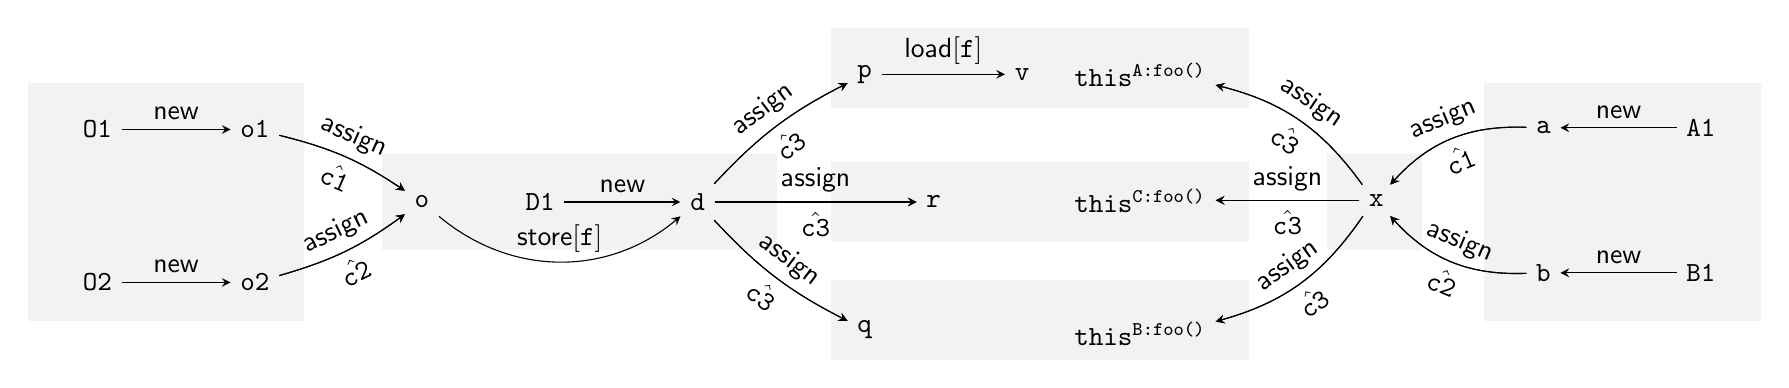
\begin{tikzpicture}
    \draw [draw=black!5, fill=black!5] (-0.3,2.2) rectangle (5.0,1.2); % A::foo
    \draw [draw=black!5, fill=black!5] (-0.3,0.5,0) rectangle (5.0,-0.5); % C::foo
    \draw [draw=black!5, fill=black!5] (-0.3,-1.0,0) rectangle (5.0,-2.0);  % B::foo
    % \draw [draw=black!5, fill=black!5] (-10.5,1.7,0) rectangle (-3.5,0.9); % main
    % \draw [draw=black!5, fill=black!5] (-10.5,-1.5,0) rectangle (-3.5,-.8); % main
    \draw [draw=black!5, fill=black!5] (-10.5,1.5,0) rectangle (-7.0,-1.5); % main
    \draw [draw=black!5, fill=black!5] (8.0,1.5,0) rectangle (11.5,-1.5); % main
    
    \draw [draw=black!5, fill=black!5] (-6.0,0.6,0) rectangle (-1.0,-0.6); % bar
    \draw [draw=black!5, fill=black!5] (6.0,0.6,0) rectangle (7.2,-0.6); % bar
    
    \node(d)[xshift=-2cm] {\texttt{d}};
    % \node(d)[left of =x, xshift=0.5cm] {\texttt{d}};
    \node(D)[left of=d, xshift=1cm, yshift=.0cm] {\texttt{D1}};
    \node(o)[left of=D, xshift=1.5cm] {\texttt{o}};
    \node(o1)[above left of=o, yshift=-1.2cm] {\texttt{o1}};
    \node(O1)[left of=o1, xshift=1cm] {\texttt{O1}};
    \node(o2)[below left of=o, yshift=1.1cm] {\texttt{o2}};
    \node(O2)[left of=o2, xshift=1cm] {\texttt{O2}};
    % \node(xc)[right of=x, xshift=-1cm] {\texttt{x\#c3}};
    \node(p)[above right of=d, yshift=-0.5cm]{\texttt{p}};
    \node(r)[right of=d]{\texttt{r}};
    \node(v)[right of=p,xshift=-1cm]{\texttt{v}};
    \node(thisA)[right of=v, xshift=-1.5cm] {$\texttt{this}^\texttt{A:foo()}$};
    \node(thisC)[below of=thisA, yshift=1.4cm] {$\texttt{this}^\texttt{C:foo()}$};
    \node(thisB)[below of=thisC, yshift=1.3cm] {$\texttt{this}^\texttt{B:foo()}$};
    \node(q)[below right of=d, yshift=0.5cm] {\texttt{q}};
    
    \node(x) [right of =thisC] {\texttt{x}};
    \node(a)[above right of=x, yshift=-1.2cm] {\texttt{a}};
    \node(A)[right of=a, xshift=-1cm] {\texttt{A1}};
    \node(b)[below right of=x, yshift=1.2cm] {\texttt{b}};
    \node(B)[right of=b, xshift=-1cm] {\texttt{B1}};

    
    \path[-stealth]
    (O1) edge[sloped] node{$\new$} (o1)
    (O2) edge[sloped] node{$\new$} (o2)
    
    (A) edge[sloped] node{$\new$} (a)
    (B) edge[sloped] node{$\new$} (b)
    
    (D) edge[sloped, above] node{$\new$} (d)
    
    (a) edge[sloped,bend right=25] node{\assign} (x)
    (a) edge[sloped,bend right=25,below] node{$\hat{\mathtt{c1}}$} (x)
    (o1) edge[sloped,bend left=10] node{\assign} (o)
    (o1) edge[sloped,bend left=10,below] node{$\hat{\mathtt{c1}}$} (o)
    
    (b) edge[sloped,bend left=25] node{\assign} (x)
    (b) edge[sloped,bend left=25,below] node{$\hat{\mathtt{c2}}$} (x)
    (o2) edge[sloped,bend right=10] node{\assign} (o)
    (o2) edge[sloped,bend right=10,below] node{$\hat{\mathtt{c2}}$} (o)
    
    (o) edge[sloped, bend right=40] node{$\store[\texttt{f}]$} (d)
    
    (d) edge[sloped,bend left=10] node{\assign} (p)
    (d) edge[sloped,bend left=10,below] node{$\hat{\mathtt{c3}}$} (p)
    
    (d) edge[sloped,bend right=0] node{\assign} (r)
    (d) edge[sloped,bend right=0,below] node{$\hat{\mathtt{c3}}$} (r)
    
    (d) edge[sloped,bend right=10] node{\assign} (q)
    (d) edge[sloped,bend right=10,below] node{$\hat{\mathtt{c3}}$} (q)
    
    % (d) edge[sloped,bend left=0] node{$\store[1]$} (x)
    % (d) edge[sloped,bend left=0,below] node{$\hat{\boxed{\mathtt{c3}}}$} (x)
    
    % (x) edge[sloped,bend right=30] node{$\assign$} ([shift={(-.1,-.2)}]xc)
    % (x) edge[sloped,bend right=30,below] node {$\check{\boxed{\mathtt{c3}}}$} ([shift={(-.1,-.2)}]xc)
    % (x) edge[sloped,bend left=30] node{$\assign$} ([shift={(-.1,.2)}]xc)
    
    (x) edge[sloped,bend right=20] node{$\assign$} (thisA)
    (x) edge[sloped,bend right=20,below] node{$\hat{\mathtt{c3}}$} (thisA)
    % (thisA) edge[sloped] node{$\load[1]$} (p)
    (p) edge[sloped] node{$\load[\texttt{f}]$} (v)
    
    (x) edge[sloped, bend left=20] node{$\assign$} (thisB)
    (x) edge[sloped, bend left=20, below] node{$\hat{\mathtt{c3}}$} (thisB)
    % (thisB) edge[sloped] node{$\load[1]$} (q)
    
    (x) edge[sloped] node{$\assign$} (thisC)
    (x) edge[sloped,below] node{$\hat{\mathtt{c3}}$} (thisC)
    % (thisC) edge[sloped] node{$\load[1]$} (r)
    ;
\end{tikzpicture}
}
% \vspace*{-2.5ex}
\caption{The PAG operated on by \manuLFC for the program given in \Cref{fig:motivatingExample}.}
\label{fig:pag2}
% \vspace*{-1ex}
\end{figure*}

% But as mentioned earlier, when an imprecise call-graph is used, precision will be lost, and when the pre-built call-graph is as precise as the one on-fly built, it means similar pointer analysis has been performed and consequently the value-flow analysis guided by grammar in-doing becomes meaningless. Not only that, because we require the graph to be static, so no matter how precise the call graph given is, it will lose all context-sensitive information contained.

Why is the precision loss?
In \manuLFC, parameter passing for a virtual callsite (\rulename{P-VCall}) is modeled identically as that at a static callsite (\rulename{P-SCall}) by  using inter-procedural \reg{assign} edges as shown in the two \manuLFC-paths given above, without being CFL-reachability-related to the receiver objects at the callsite. As a result,
\manuLFC does not really understand that 
under context [\callsitefont{c1}], in which case 
 \texttt{x} points to the receiver \commentfont{A1},
only 
the first \manuLFC-path above can be established.

%makes the parameter passing from \texttt{d} to \texttt{p} reachable under only \texttt{c1} and unreachable under \texttt{c2}. However, the only edge from \texttt{d} to \texttt{p} that could be added to PAG is \texttt{d}$\xrightarrow[\hat{\texttt{c3}}]{}$p, which means 
%$\pointsto(\csabstraction{\mathtt{d}}{ctx}) \subseteq \pointsto(\csabstraction{\mathtt{p}}{\mathtt{c3}\mdoubleplus ctx})$ where $ctx$ is any context of \texttt{foo()} (not only \texttt{c1} but also \texttt{c2}). That is why \Cref{eq:LFCPathCGPreciseII} is valid in traditional \manuLFC. 

\begin{comment}
The reason for such precision loss case is that the PAG constructed only require the context-insensitive call relation of a callgraph, so no matter how precise the call graph given is, it will lose all context-sensitive information contained. For example, \texttt{x} (line~17) points to \commentfont{A1} under context \texttt{c1}, which makes the parameter passing from \texttt{d} to \texttt{p} reachable under only \texttt{c1} and unreachable under \texttt{c2}. However, the only edge from \texttt{d} to \texttt{p} that could be added to PAG is \texttt{d}$\xrightarrow[\hat{\texttt{c3}}]{}$p, which means 
$\pointsto(\csabstraction{\mathtt{d}}{ctx}) \subseteq \pointsto(\csabstraction{\mathtt{p}}{\mathtt{c3}\mdoubleplus ctx})$ where $ctx$ is any context of \texttt{foo()} (not only \texttt{c1} but also \texttt{c2}). That is why \Cref{eq:LFCPathCGPreciseII} is valid in traditional \manuLFC. 
\end{comment}

%We show that pointer analysis guided by \manuLFC on a PAG constructed with rules in \Cref{fig:manucflpag} but using a imprecise pre-build callgraph will be imprecise than \kcs{k}. 

If \manuLFC uses a less precise 
 call graph, which is pre-built by, say,  CHA \cite{dean1995optimization}, then
 \texttt{C:foo()} will also be identified as a target method at callsite {\texttt{c3}} (line~17). In this case, \texttt{r} is found to point to \commentfont{D1}
 due to ${\color{purple} \texttt{D1}}\xrightarrow{\new}\texttt{d}\xrightarrow[\hat{\mathtt{c3}}]{\assign}
\texttt{r}$, but
its points-to set is empty by \kcs{2} (not  listed in \Cref{table:kcfaresults}).
 
\begin{comment}
\begin{equation} \scriptsize
  \centering
\label{eq:LFCPathCGImprecise}
\begin{tabular}{l}
\commentfont{D}$\xrightarrow{\new}
\texttt{d}\xrightarrow[\hat{\mathtt{c3}}]{\assign}
\texttt{r}
$
\end{tabular}
\end{equation}
\end{comment}

 


\paragraph{\bf Using a Call Graph Constructed On the Fly}
\label{sec:LFC+fly}
In solving \kcs{k} with \manuLFC on-demand \cite{sridharan2006refinement,yan2011demand,shang2012demand},
every method that is invoked at a virtual callsite is dispatched  only 
under a specific context, resulting in on-the-fly call graph construction (which
implies that the \pag edges related to a call are not always
fixed but provided to \manuLFC when the call is analyzed under a given context). 

Consider again ``\inline{x.foo(d); // c3}'' (line~17) in \Cref{fig:motivatingExample}.
We can now establish that the path in
\Cref{eq:LFCPathCGPreciseI} is an \manuLFC-path but the   
path  in \Cref{eq:LFCPathCGPreciseII} is not, so that
we can conclude precisely that \texttt{v} points to \commentfont{O1} only.
In the former case, we reach \texttt{d} under context [\texttt{c1}] 
and then issue a points-to query to find what
\texttt{x}  points to  under [\callsitefont{c1}]. As \texttt{x} is found to point to \commentfont{A1} in this case
(causing
\texttt{A:foo()} to be invoked at callsite \callsitefont{c3}), we will continue traversing the
remaining \manuLFC-path from \texttt{d}
and conclude that \texttt{v} points to \commentfont{O1}. In the latter case,
reaching
\texttt{d} under  [\callsitefont{c2}] reveals \texttt{B:foo()} as the target at callsite
\callsitefont{c3} instead
(as \texttt{x} points to \commentfont{B1} under [\callsitefont{c2}]), thereby causing 
$\xrightarrow[\hat{{\mathtt{c3}}}]{\assign} \mathtt{p} \xrightarrow{\load[\texttt{f}]} \mathtt{v}$
not 
 to be traversed.

\begin{comment}
we  \cite{sridharan2005demand, sridharan2006refinement} initiate an additional algorithm to compute which objects are pointed by \texttt{x} under context [\texttt{c2}] and eliminate the remaining part, i.e., $\xrightarrow[\hat{\mathtt{c3}}]{\assign} \mathtt{p} \xrightarrow{\load[f]} \mathtt{v}$, of \Cref{eq:LFCPathCGPreciseII} due to $\pointsto{\csabstraction{\mathtt{x}}{[\mathtt{c2}]}} = \{\csabstraction{{\color{purple} \mathtt{B}}}{\emptyctx}\}$ (\Cref{table:kcfaresults}).  


\begin{equation*}
  \centering
\begin{tabular}{l}\scriptsize
\commentfont{O2}$\xrightarrow{\new}
\texttt{o2}\xrightarrow[\hat{\mathtt{c2}}]{\assign}
\texttt{o} \xrightarrow{\storefield{f}} \texttt{d}
\xrightarrow{\inew}$ \commentfont{D} 
$ \xrightarrow{\new} \texttt{d}
$
\end{tabular}
\end{equation*}
\end{comment}


%\begin{wrapfigure}{r}{4.0cm} 
\begin{figure}[h]
%\vspace*{-1.5ex}
\begin{center}
\begin{mdframed}[
align=center,
usetwoside=false,
%innermargin =-2ex,
%  rightmargin=-1cm,
 rightmargin=8.5cm,
innerleftmargin=4.0ex,
%innerrightmargin=-1.0ex,
% innerrightmargin=-00.0ex
innertopmargin=0.2ex,
innerbottommargin=0.2ex
]
\begin{lrbox}{\mybox}
\begin{lstlisting}[language=java, numbers=none, otherkeywords = {null}]
D d = new D(); // D1
if (...)
  d.f = a = new A(); // A1 
else
  d.f = b = new B(); // B1
A x = d.f;
x.foo(null); // c
\end{lstlisting}
\end{lrbox}
\scalebox{1}{\usebox{\mybox}}
\end{mdframed}
\end{center}
%\vspace*{-2ex}
\caption{A small example.
\label{fig:recvobj}}
% \vspace*{-2ex}
\end{figure}

While \manuLFC can be used to solve \kcs{k} on-demand (more precisely than if 
a pre-built call graph is used), some precision loss may occur
when a callsite has several dispatch targets under a common calling context. Consider the  
 code snippet given in \Cref{fig:recvobj} (which reuses classes \texttt{A}, \texttt{B}, and \texttt{D} from \Cref{fig:motivatingExample}).
If we ask a separate call graph construction algorithm to find on-demand the  
target methods  at ``\inline{x.foo(null)}''
under any context invoking this piece of code,  both
 \texttt{A:foo()} and \texttt{B:foo()} will be returned. If we then reason about
 CFL-reachability 
with \manuLFC, we will obtain:
{
\setlength{\abovedisplayskip}{3ex}
\begin{equation} 
% \footnotesize
  \centering
\label{eq:LFCPathCGOnFlyI}
\begin{tabular}{l} 
\commentfont{A1}$\xrightarrow{\new} \texttt{a} \xrightarrow{\store[\texttt{f}]} \texttt{d}
\xrightarrow{\inew}$ \commentfont{D1} 
$ \xrightarrow{\new} \texttt{d}
\xrightarrow{\load[\texttt{f}]} \texttt{x}
\xrightarrow[\hat{\mathtt{c}}]{\assign} \mathtt{this}^{\texttt{A:foo()}}$
\end{tabular}
% \vspace*{-2ex}
\end{equation}
}
{
\setlength{\belowdisplayskip}{6ex}
\begin{equation} 
% \footnotesize
  \centering
\label{eq:LFCPathCGOnFlyII}
\begin{tabular}{l} 
\commentfont{B1}$\xrightarrow{\new} \texttt{b} \xrightarrow{\store[\texttt{f}]} \texttt{d}
\xrightarrow{\overline{\new}}$ \commentfont{D1} 
$ \xrightarrow{\new} \texttt{d}
\xrightarrow{\load[\texttt{f}]} \texttt{x}
\xrightarrow[\hat{\mathtt{c}}]{\assign} \mathtt{this}^{\texttt{A:foo()}}$
\end{tabular}
%\vspace*{-1ex}
\end{equation}
}
%\hspace{-1.ex}
Therefore,
both \commentfont{A1} and \commentfont{B1} will flow to 
$\texttt{this}^{\texttt{A:foo}}$ although \commentfont{B1} is spurious by \rulename{I-VCall}.
%(since it cannot be a receiver of \texttt{A:foo()}).  
%Similarly, both \texttt{A} and \texttt{B} will also flow to 
%$\texttt{this}^{\texttt{B:foo}}$ even though \texttt{A}  now becomes spurious. 

We see a loss of   precision at such a virtual callsite since \manuLFC does not handle
its receiver variable differently from its other arguments (\rulename{P-VCall}) unlike the Andersen-style inclusion-based formulation
 (\rulename{I-VCall}). 
 %Resorting to type filtering,
 Removing  spurious receiver objects such as \commentfont{B1} by brute force as discussed above
(specified formally by 
 neither \manuLFC nor the call graph construction algorithm used) is
ad hoc.
Indeed, the \manuLFC-based on-demand algorithm for solving \kcs{k} 
(released 
by the authors of \manuLFC \cite{sridharan2006refinement} in \soot~\cite{vallee2010soot} and used by many others
 \cite{xu2009scaling, shang2012demand} in the past 15 years) suffers still from this
problem.


%A separate handling of receiver and normal arguments (similar to \rulename{I-Call}) is often captured in the additional algorithm to support such difference. Note that this problem cannot be solved by a simple type filtering for "\texttt{this}" variables due to the existence of "special" calls.


% Like inference rules, we can easily get something like $(\texttt{v}, \texttt{c1}) -> (\texttt{p}, \texttt{c3c1})$
% and $(\texttt{v}, \texttt{c2}) -> (\texttt{q}, \texttt{c3c2})$, which means \texttt{v} under context \texttt{c1} is assigned to \texttt{p} under context \texttt{c3c1} and \texttt{v} under context \texttt{c2} is assigned to \texttt{q} under context \texttt{c3c2}, but this is what $L_{FC}$ failed to express. This inaccurate statement will lead to inaccurate conclusions when doing some CFL-based optimization and analysis.

% An instance is that in \textsc{Selectx}~\cite{lu2021selective}, the authors conservatively verify the necessity of context-sensitivity by reasoning CFL path of a points-to relation with all nodes infecting its reachability on it. However, due to the characteristics analyzed above, this approach is not conservative in fact, which fails to preserve precision.
% In the following, we will discuss it and give a feasible approach to solve the problem of passing parameters during on-fly call-graph building, and verify it with a selective \kcs{k} solution.

\begin{comment}
\subsection{Discussion}
\label{subsec:discussion}

\subsubsection{rec2this}
The receiver of a call is a special argument used to implement polymorphism according to its type. Except for dispatch, its value follows the same rules as regular arguments when passed. In traditional CFL, the value flow from receiver to "this" parameter is no other than that from a regular argument to its corresponding parameter. 
However, the two are indeed different in the algorithm. In the inference rules, a receiver object only goes into the method dispatched by itself, whereas an argument goes into all methods dispatched at this call-site.


\begin{figure}[htbp]
	\centering
    \begin{subfigure}{.525\linewidth}
\begin{lrbox}{\mybox}   
\begin{lstlisting}[language=java, basicstyle=\small]
class A {
    void foo() {}
}

class B extends A {
    void foo() {}
}

\end{lstlisting}
\end{lrbox}
\scalebox{0.8}{\usebox{\mybox}} 
    \end{subfigure}
    \begin{subfigure}{.465\linewidth}
\begin{lstlisting}[language=java, firstnumber=8, basicstyle=\small]
...
x.foo();
...
\end{lstlisting}
    \end{subfigure}
	\caption{An example for illustrating receiver-to-this parameter passing imprecisely handled by
$L_{F}$.}
	\label{fig:rec2this}
\end{figure}

For example, consider a callsite \texttt{x.foo()} shown in \cref{fig:rec2this}.
Class \texttt{A} defines method \texttt{foo()}, which is overridden by its subclass \texttt{B}.
A correct points-to relation should be $\texttt{this}^\texttt{A:foo}$ points to only \texttt{A1} and $\texttt{this}^\texttt{B:foo}$ points to only \texttt{B1}. However, due to the lack of provision 
in $L_{FC}$ on how the call graph should be constructed \emph{during the CFL-reachability-based pointer analysis}, they cannot be distinguished, no matter how precise the call graph provided by the pre-analysis is.

%type filtering not work. object sensitivity?

In the inference rules, as can be seen in \cref{rule:cfapta}, receiver and other arguments follow different rules to handle this issue. 


\end{comment}

%\vspace*{-1.5ex}

\paragraph{Discussion}
\label{sec:manuLFC+sep}

When solving \kcs{k},
 \manuLFC relies on a separate algorithm for performing 
 call graph construction. In addition to cause
 \kcs{k} to lose precision as discussed above, \manuLFC
 suffers from another limitation, as it fails to
capture all the value-flow paths traversed for a program during the pointer  analysis (regardless of whether its call graph is built in advance or on the fly).  


Consider again how ``\inline{x.foo(d)}'' (line~17) in \Cref{fig:motivatingExample} is analyzed. To perform parameter passing for \texttt{d} at the callsite
according to the Andersen-style  inclusion-based
formulation (\rulename{I-VCall}), we must first find the  methods dispatched on
the receiver objects pointed by \texttt{x}
and then perform the actual parameter passing (from  \texttt{d} to \texttt{p} if
\texttt{A:foo()} is dispatched and
\texttt{d} to \texttt{q} if
\texttt{B:foo()} is dispatched). However, with \manuLFC,  parameter passing (realized by inter-procedural
\reg{assign} edges (\rulename{P-VCall})) is both conceptually and algorithmically
disconnected with dynamic dispatch at the callsite, without being CFL-reachability-related
to its receiver objects, as also reviewed by the PAG in \Cref{fig:pag2}.

\hl{As \manuLFC does not incorporate callgraph construction within its formulation},
any  analysis that reasons about  CFL-reachability in terms of \manuLFC  may
make some optimization decisions 
that reduce  the precision of \kcs{k} (among others). For example, a recent
pre-analysis  \cite{lu2021selective} that is developed based
on \manuLFC for accelerating \kcs{k} with selective context-sensitivity  will   cause \kcs{k} to always lose precision.

\begin{comment}
Conceptually, for a call $\mathtt{x = } ~ a_0.\mathtt{m}(a_1,..., a_r) ~ \mathtt{//~ c}$, whether the parameter passing edge from
$a_i$ to $p_i^{m'}$ ($i \in [0, r]$) exists is actually determined by whether $a_0$ can point to some object \texttt{o} 
such that $m' = ~$\lookup(\texttt{m}, \texttt{o}$)$. The path of parameter passing (return) in traditional grammar is simply an entry (exit)
edge (\rulename{P-Call}) that does not relate to the receiver, so it can often only rely on some pre-analysis to provided a call-graph to build these inter-procedure PAG edges. As shown above, the imprecision of pre-analysis could affect the precision of \manuLFC. 


However, such an additional algorithm is often not feasible for doing some CFL-based optimization and analysis. For instance, the recent context selection approach, \selectx~\cite{lu2021selective}, verifies the necessity of context-sensitivity for all variables and objects in a pre-analysis stage by reasoning CFL path conservatively. The additional expensive dispatching algorithm would make \selectx infeasible as a lightweight pre-analysis. As a result, \selectx relies on a pre-build callgraph for PAG construction and fails to select some precision-critical variables and objects to be analyzed context-sensitively due to a lack of on-fly dispatching mechanism in \manuLFC.
\end{comment}

\begin{comment}
\begin{figure}[t]
		\centering
		\resizebox{0.9\width}{0.9\height}{
			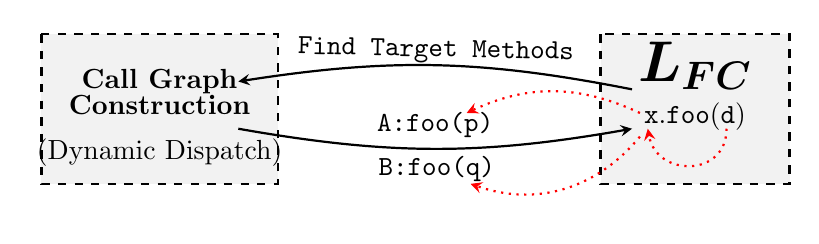
\begin{tikzpicture}
			\def\xc{3.5}
			\def\yc{0}
			\def\dist{2.8}
			\draw [draw=black, dashed, thick, fill=black!5] (-3.5 + \xc,0.7 + \yc,0) rectangle (-0.5 + \xc, -1.2 + \yc); % call graph construction
			\draw [draw=black, dashed, thick, fill=black!5] (0.8 + \xc + \dist,0.7 + \yc,0) rectangle (3.2 + \xc + \dist,-1.2 + \yc); % LFC
			\node (cg) at(-2 + \xc, 0.1 + \yc) {\bf Call Graph};
			\node (con) at (-2 + \xc, -0.2 + \yc) {\bf Construction};
			\node (vir) at (-2 + \xc, -0.8 + \yc) {(Dynamic Dispatch)};
			\node (l) at (2 + \xc + \dist, 0.3 + \yc) {\huge $\boldsymbol{L_{FC}}$};
			\node (c) at (2 + \xc + \dist, -0.35 + \yc) {$\mathtt{x.foo(d)}$};
			\node at (1.5 + \xc, -0.45 + \yc) {$\texttt{A:foo(p)}$};
			
			\path[-stealth]
			
			(1.2 + \xc + \dist, 0.0 + \yc) edge[sloped, thick, bend right=10] node[xshift=-0.0cm, yshift=-0.1cm]{\texttt{Find Target Methods}} (-1.0 + \xc, 0.1 + \yc) % find targets
			
			(-1.0 + \xc, -0.5 + \yc) edge [sloped, thick, bend right=10] node[xshift=0.02cm, yshift=-0.55cm]{$\texttt{B:foo(q)}$} (1.2 + \xc + \dist, -0.5 + \yc) % cg to x.foo

			(2.4 + \xc + \dist, -0.5 + \yc) edge[red, thick, dotted, in=-80, out=-90, loop, looseness=1.6, below] node[yshift=0.35cm]{{\Large \ScissorLeft}} (1.4 + \xc + \dist, -0.5 + \yc) % d to x
			
			(1.3 + \xc + \dist, -0.3 + \yc) edge[red, thick, dotted, sloped, bend right=25] node[yshift=-0.34cm]{{\Large \ScissorLeft}} (-0.9 + \xc + \dist, -0.3 + \yc) % x to p
			
			(1.3 + \xc + \dist, -0.6 + \yc) edge[red, thick, dotted, sloped, bend left=35] node[yshift=-0.34cm]{{\Large \ScissorLeft}} (-0.85 + \xc + \dist, -1.2 + \yc) % x to q
			;
			\end{tikzpicture}
		}
\vspace*{-3.5ex}
		\caption{Disconnection in the value flows between parameter passing in \manuLFC and
		dynamic dispatch at a virtual callsite.}
		\label{fig:MissingCGValueFlow}
\vspace*{-1.5ex}
	\end{figure}
\end{comment}

\subsubsection{\LFCR: Necessity, Challenges, and Our Solution}
\label{subsubsec:challenges}




\begin{comment}
Naturally, one may attempt to exploit Melski-Reps reduction \cite{melski2000interconvertibility} to obtain the new CFL-reachability formulation from their corresponding inclusion-based formulation. Unfortunately, the new CFL-reachability formulation does not have an equivalent set-constraint formulation as its form would be an intersection of several CFLs which has been proven to be undecidable \cite{reps2000undecidability}.
\end{comment}

\hl{Our primary contribution in this research is demonstrating the feasibility of incorporating on-the-fly callgraph construction into the specification of \kcs{k} using CFL-reachability.} In particular,
we introduce \LFCR (as the intersection of three CFLs)
as the first % complete 
CFL-reachability formulation of
\kcs{k} with built-in call graph construction, thereby overcoming the limitations of
\manuLFC (as the intersections of two CFLs) discussed above. It is worth emphasizing that
\LFCR operates on a new
PAG representation that is fundamentally different from the one operated on by \manuLFC. As the secondary contribution of this research, we demonstrate the utility of \LFCR
by introducing the first precision-preserving pre-analysis
for accelerating \kcs{k} with selective context-sensitivity. As discussed above, a recent \manuLFC-based
pre-analysis always loses precision.

\begin{comment}
We have designed \LFCR as the intersection of three CFLs to facilitate 
\LFCR-enabled CFL-reachability analyses. By noting that
\kcs{\infty} is undecidable and thus both the \manuLFC- and \LFCR-path
problems are undecidable (implying that either is a context-sensitive language
rather than a single CFL) \cite{reps2000undecidability}, 
\end{comment}

When developing \LFCR, we are required to reason about CFL reachability  to 
support parameter passing  prescribed by \kcs{k}. For
a virtual call $\texttt{r}.\texttt{m}(a_1, \dots, a_n)$ at callsite 
\textcolor{red}{c}, passing any of its
arguments $a$ to its corresponding
parameter $p$ of a   target method $m'$ that is yet to be discovered at this
callsite by \LFCR itself
under a given context $\CC$ must be done by establishing a CFL-reachability path in
a PAG representation of the program, starting from $a$, passing through the receiver variable $\texttt{r}$ to trigger dynamic dispatch, and
finally, ending at $p$, which is the corresponding parameter of $m'$ that is dispatched based on the
dynamic type of the object pointed by \texttt{r}
under the given context $\CC$. Relating $a$ to $\texttt{r}$   is non-trivial
if $a=a_i$ (for some $i$), i.e., $a\neq \texttt{r}$. In addition, in a CFL-reachability formulation, some
context elements in $\CC$ are usually consumed (i.e., balanced out according to \manuLC given in
\Cref{eqn:callsiteLC}) during the traversal for performing
 dynamic dispatch  and must thus be restored in order to enable \texttt{d} to be
passed to \texttt{p} under still the same given context \CC.
Below we list 
three challenges faced in handling this parameter passing task during the
on-the-fly call graph construction: 
 \begin{itemize}[leftmargin=*]
 \item  \challenge{1}.  How do we pass \texttt{r} to the  ``this'' variable of a target method invoked at callsite \textcolor{red}{c} 
 precisely (by avoiding
the precision loss illustrated with the code given in \Cref{fig:recvobj})?
 
  \item  \challenge{2}.  
  How do we establish a CFL-reachability path in a PAG representation of the program
  from   $a_i$ to $p_i$ passing through \texttt{r} in order to trigger
  dynamic dispatch during the course of parameter passing, where
  $p_i$ is the $i$-th parameter of a target method $m'$ discovered 
  at callsite \textcolor{red}{c} under  $\CC$?
 % passing for a set $T_{\scriptsize \LFCR}$ of    target methods discovered by \LFCR at callsite
 % \textcolor{red}{c}, such that $T_{\scriptsize \LFCR} \supseteq T_{\kcs{k}}$, where $T_{\kcs{k}}$ is  the set of target methods that are found by   \kcs{k} at callsite  \textcolor{red}{c} under context \textcolor{red}{c}?
 
 %or more specifically $\textcolor{red}{c} \mdoubleplus  \CC$, i.e., $[\textcolor{red}{c},c_1,...,c_n]$?  

 %\item {\bf CHL3.} Where do we perform dynamic dispatch for a virtual callsite during the
% CFL-reachability traversal for finding its receiver objects: at this callsite or the allocation sites where these receiver objects are created? 
 
 \item \challenge{3}. How
 do we ensure we can pass $a_i$ to $p_i$ for the target method $m'$ invoked 
at callsite \textcolor{red}{c}
 with a (correct) context abstraction that represents parameter passing
 for callsite \textcolor{red}{c}
  under $\CC$?
 
 %How do we ensure that parameter passing at a virtual callsite (with dynamic dispatch  performed by \LFCR itself) happens correctly with respect to \kcs{k} \cite{shivers1991control}?

%as in the demand-driven\manuLFC-based formulation \cite{sridharan2006refinement} (with dynamic dispatch being  performed by separate algorithm)?

 
 %\item {\bf CHL5.} 
 %How do we 
% ensure that the contexts
%just before and after parameter passing at a virtual callsite are identical when
%CFL-reachability-enabled
%dynamic dispatch happens in between?
 
 %How to ensure the context after dispatching are same as the traditional \manuLFC formulation that has an oracle for telling where to dispatch?   
  \end{itemize}

We  now give a high-level  overview of our solution  by using our motivating example 
(\Cref{fig:motivatingExample}). To support on-the-fly call graph construction
by itself,
\LFCR operates on a new PAG representation  shown in \Cref{fig:pag1}, which differs fundamentally from the PAG (\Cref{fig:pag2}) operated on by \manuLFC. In our formulation, we find that \texttt{v} points to \commentfont{O1} only due
to the existence of the following unique path from \commentfont{O1} to \texttt{v}, with the underlying technical details being explained
in \Cref{sec:CFL}:
{
\setlength{\abovedisplayskip}{4ex}
%\setlength{\belowdisplayskip}{1.5ex}
\begin{equation}
  \centering
\label{eq:ex-patho1-to-v}
\begin{tabular}{l} 
% \footnotesize
\vspace*{1ex}
\begin{tikzpicture}[-, remember picture,overlay]
%line
\def\lx{11.7}\def\ly{0.1}
\def\dy{-0.80}
\def\nx{-.4}\def\ny{-1.55}
\def\offset{0.25}
%rectangle height
\def\chIIaabove{0.5}\def\chIIabelow{0.5}
\def\chIIbabove{0.4}\def\chIIbbelow{0.5}
\def\chIIIaabove{0.5}\def\chIIIabelow{0.5}
\def\chIIIbabove{0.4}\def\chIIIbbelow{0.5}
\def\chIVaabove{0.6}\def\chIVabelow{0.6}
\def\chIVbabove{0.5}\def\chIVbbelow{0.6}
%rectangle location
\def\chIIastartx{\lx-4.55}
\def\chIIIastartx{\lx-2.86}
\def\chIIIaendx{\lx-.1}
\def\chIIIbstartx{\nx}
\def\chIIbstartx{\nx+6.15}
\def\chIIbendx{\nx+9.1}

\draw [draw=\chIVcolor, fill=\chIVcolor] (\chIIastartx-.1,\ly+\chIVaabove) rectangle (\chIIIaendx+.2,\ly-\chIVabelow); % CH4a-blue1
\draw [draw=\chIVcolor, fill=\chIVcolor] (\chIIIbstartx-.1,\ny+\chIVbabove) rectangle (\chIIbendx+.22,\ny-\chIVbbelow); % CH4b-blue2
\draw [draw=\chIIcolor, fill=\chIIcolor] (\chIIastartx,\ly+\chIIaabove) rectangle (\chIIIastartx,\ly-\chIIabelow); % CH2a-red1
\draw [draw=\chIIcolor, fill=\chIIcolor] (\chIIbstartx,\ny+\chIIbabove) rectangle (\chIIbendx+0.12,\ny-\chIIbbelow); % CH2b-red2
\draw [draw=\chIIIcolor, fill=\chIIIcolor] (\chIIIastartx,\ly+\chIIIaabove) rectangle (\chIIIaendx,\ly-\chIIIabelow); % CH3a-green1
\draw [draw=\chIIIcolor, fill=\chIIIcolor] (\chIIIbstartx+0.1,\ny+\chIIIbabove) rectangle (\chIIbstartx,\ny-\chIIIbbelow); % CH3b-green2


\draw(\lx-\offset, \ly) -- (\lx, \ly) -- (\lx, \dy);
\draw[dashed] (\lx, \dy) -- (\nx,\dy);
\draw(\nx,\dy) -- (\nx, \ny);
\draw[->] (\nx, \ny) -- (\nx+\offset, \ny);
\end{tikzpicture}
\commentfont{O1}$\xrightarrow{\new[\texttt{O}]}
\texttt{o1}\xrightarrow[\hat{\mathtt{c1}}]{\assign}
\texttt{o} \xrightarrow{\storefield{f}} \texttt{d}
\xrightarrow{\inewfield{\texttt{D}}}$ \commentfont{D1} 
$\xrightarrow{\new[\texttt{D}]} 
\texttt{d}$ $\xrightarrow[\hat{\boxed{\texttt{c3}}}]{\store[1]}\texttt{x}\xrightarrow[\check{\texttt{c1}}]{\iassign}\texttt{a} $ $\xrightarrow{\inewfield{\texttt{A}}}$\commentfont{A1} \\[6ex]
% \footnotesize 
$\xrightarrow{\new[\texttt{A}]}\texttt{a}\xrightarrow[\hat{\texttt{c1}}]{\assign}\texttt{x} \xrightarrow[\check{\boxed{\texttt{c3}}}]{\assign} \texttt{x\#c3}$ $\xrightarrow[\hat{\texttt{c3}}]{\indispatch[\texttt{A}]}\texttt{this}^\texttt{A:foo()}
\xrightarrow{\load[1]}\texttt{p}
    \xrightarrow{\load[\texttt{f}]} \texttt{v}$ \\[3ex]
% \begin{tikzpicture}[-, remember picture,overlay]
% \def\lx{7.1}\def\ly{.95}
% \def\dy{.45}\def\ny{.068}
% \draw(\lx, \ly) -- (\lx+.1, \ly) -- (\lx+.1, \dy);
% \draw[dashed] (\lx+.1, \dy) -- (-.12,\dy);
% \draw(-.12,\dy) -- (-.12, \ny);
% \draw[->] (-.12, \ny) -- (0.06, \ny);
% \end{tikzpicture}
% \footnotesize 
% $\xrightarrow[\hat{\texttt{c3}}]{\indispatch[\texttt{A}]}\texttt{this}^\texttt{A:foo()}
% \xrightarrow{\load[1]}\texttt{p}
%     \xrightarrow{\load[\texttt{f}]} \texttt{v}$
\end{tabular}
\end{equation}
}

This path represents the flow of \commentfont{O1} to \texttt{v} by passing a sequence of
two calls,  ``\inline{bar(a,o1); // c1}'' and ``\inline{x.foo(d); // c3}''. Consider the
parameter passing for \texttt{d} under  context $\CC=[\texttt{c1}]$ at ``\inline{x.foo(d); // c3}'', which has only one target \texttt{A:foo()}.
 Instead of passing \texttt{d} to \texttt{p} directly via  one inter-procedural
\assign edge 
$d\xrightarrow[\hat{{\mathtt{c3}}}]{\assign} \mathtt{p}$
as in \manuLFC (\Cref{eq:LFCPathCGPreciseI}), which is illustrated in
\Cref{fig:pag2}, since \manuLFC requires  \texttt{A:foo()}
 to be found separately outside \manuLFC, \LFCR passes \texttt{d} to \texttt{p} indirectly
 via a sequence of PAG edges, along the path given in
 \Cref{eq:ex-patho1-to-v} (shown also in  \Cref{fig:pag1}),  by discovering this dispatch target dynamically during
 the sub-path from \texttt{d} to \texttt{p}. Briefly, we address 
 \challenge{1} by requiring $\new[\texttt{A}]$ to be matched with $\indispatch[\texttt{A}]$.
 We address \challenge{2} by first storing \texttt{d} into a special field of \texttt{x}
 to trigger dynamic dispatch at this callsite 
 and then loading it from the same special field of $\texttt{this}^\texttt{A:foo()}$
 into \texttt{p} later (with the two sub-paths highlighted in
 \crule[\chIIcolor]{1.5ex}{1.5ex}). In addition, we
 perform dynamic dispatch correctly at this callsite under 
 $\CC=[\texttt{c1}]$ (with the sub-path highlighted in \crule[\chIIIcolor]{1.5ex}{1.5ex}) as
 in the case of \manuLFC. We address \challenge{3} by passing \texttt{d} to \texttt{p}
 also correctly under  [\texttt{c3},\texttt{c1}], where \texttt{c3}  records the  callsite as in
 \manuLFC (\Cref{eq:LFCPathCGPreciseI}) for which parameter passing takes place
 and \texttt{c1} signifies further the
 context under which the receiver object \commentfont{A1} flows into the receiver
 variable \texttt{x} at this callsite
  (with the sub-path highlighted in \crule[\chIVcolor]{1.5ex}{1.5ex}). The significance
  of the two below-edge labels,
  $\hat{\boxed{\texttt{c3}}}$ and $\check{\boxed{\texttt{c3}}}$, in addressing \challenge{3} cannot be
  over-emphasized. This ensures that if we start dynamic dispatch at callsite 
  \texttt{c3} under context $\CC=[\texttt{c1}]$, we will always return
  to the same callsite    under the same context 
  even though  $\texttt{c1}$ is lost (i.e., balanced out due to
  $\hat{{\texttt{c1}}}\check{{\texttt{c1}}}$) just after
  $\mathtt{x}\xrightarrow[\check{{\mathtt{c1}}}]{\iassign} \mathtt{a}$ at the beginning of the
  traversal for performing
  dynamic dispatch at callsite \texttt{c3}.
  To address  \challenge{1} -- \challenge{3}, we
  have designed \LFCR to be the intersection of three CFLs operating on a new
  PAG representation as described below.

% \section{\texorpdfstring{\LFCR}\,: Design and Insights}
\label{sec:CFL}

When solving a CFL-reachability problem with a CFL, the CFL and its underlying graph
structure are always inter-connected and carefully designed together. To break their cyclic
dependencies, we first describe how to represent a program with a new \pag representation 
to facilitate on-the-fly call graph construction
(\Cref{subsec:newPAG}). We then
formalize \LFCR by explaining how we address the three challenges
(\challenge{1} -- \challenge{3}) and providing some insights
in understanding its design (\Cref{subsec:newCFLs}).
% In \Cref{subsec:discussion}, we discuss 
% some topics related to our new formulation. 


\subsection{Pointer Assignment Graph} 
\label{subsec:newPAG}

%Like previous pointer analyses formulated in CFL-reachability \cite{sridharan2005demand, sridharan2006refinement, lu2019precision, lu2021eagle}, our formulation also operates on a graph representation of the program, known as \textit{pointer assignment graph} (\pag). 

For a program, we use the rules given in 
\Cref{fig:newcflpag} to build a \pag representation for \LFCR. We first introduce
these rules briefly by highlighting their differences  from those adopted by \manuLFC
(\Cref{fig:manucflpag}) 
for building an \manuLFC-oriented PAG representation. We then illustrate these rules with an example.
Note that one is expected to develop a reasonably good understanding of this new PAG representation before 
examining the three CFLs used for defining
\LFCR later.
%, whose nodes 
%represent variables and heap objects, and whose edges represent the value flows through 
%assignments. 

As in the case of \manuLFC (\Cref{fig:manucflpag}), the inverse of a PAG edge
is not given
explicitly. For each \pag edge 
$x\xrightarrow[c]{\ell}y$, its inverse edge is defined as  
$y\xrightarrow[\overline{c}]{\overline{\ell}}x$ as in \manuLFC exactly  (\Cref{subsubsec:CFLReachability}),
except that 
a below-edge label can also be $\hat{\boxed{c}}$ or $\check{\boxed{c}}$
(in addition to $\hat{{c}}$ and $\check{{c}}$), in which case,
$\overline{\hat{\boxed{c}}}=\check{\boxed{c}}$ and $\overline{\check{\boxed{c}}}=\hat{\boxed{c}}$, where $c$ identifies a  callsite.
To trigger dynamic dispatch at a callsite $c$, an edge with a boxed below-edge label also represents conceptually 
a new kind of inter-procedural value-flow entering into (marked by 
$\hat{\boxed{c}}$)
or exiting from (marked by 
$\check{\boxed{c}}$) from a method invoked at  $c$. Such boxed below-edge labels are
introduced for addressing \challenge{3} only and their significance will become clear
in \Cref{subsubsec:newLR}.

%implying that the concepts
%of entry and exit contexts  for inter-context
%value-flow edges are swapped if they are
%  traversed inversely. 



 

%The rules for adding $\mathtt{y} 
%\xrightarrow{\assign} \mathtt{x}$, $\mathtt{y} \xrightarrow{\loadfield{f}} \mathtt{x}$, and 
%$\mathtt{y} \xrightarrow{\storefield{f}} \mathtt{x}$,
%which are also used in earlier work
%\cite{sridharan2005demand, sridharan2006refinement, lu2019precision, lu2021eagle}, 

% $\tau$ is a placeholder used in $L_C$ for context recovery, which will be introduced shortly.  


\begin{figure}[t]
\begin{center}
% \vspace*{-1ex}
% \begin{adjustbox}{width=1\linewidth}
\begin{tabular}{c}
			\ruledef{
				 \mathtt{x = \mathsf{\mathbf{new}} ~ T} ~ { \mathtt{//~O}}
			}{
				O \xrightarrow{\new[\texttt{T}]} \mathtt{x} 
				% \rulespace
				% \mathtt{o} \xrightarrow[\tau]{\typefound[t]} \mathtt{o}
			}
		 \rulename{C-New} 
		 \quad
			\ruledef{
			    \mathtt{x = y} 
			}{
				\mathtt{y} \xrightarrow{\assign} \mathtt{x}
			}
			\rulename{C-Assign}
			 \\[6ex]
	 		\ruledef{
            			    \mathtt{x = y.f} 
            			}{
            				\mathtt{y} \xrightarrow{\load[\texttt{f}]} \mathtt{x}
            			}
        	 \rulename{C-Load}
        	 \quad
			\ruledef{
			    \mathtt{x.f = y} 
			}{
				\mathtt{y} \xrightarrow{\store[\texttt{f}]} \mathtt{x} 
			}
			 \rulename{C-Store}
             \\[6ex]
        %      \ruledef{
        %     			}{
        %     				% 			\mathtt{this}^{m} \xrightarrow{\load[i]} \mathtt{p_i^m}
        %     							\mathtt{m} \xrightarrow{\assign} \mathtt{this^m}
        %     			}
        
        % 	 \rulename{This}
        %      \quad
   
             			\ruledef{
			   \mathtt{x = } ~ \mathtt{m}(a_1, \dots, a_n) ~ \mathtt{//~ c} 
			}{
			\rulespace \forall \ i \in [1, n]: a_i \xrightarrow[\hat{c} ]{\assign} p_i^{\mathtt{m}}
			\rulespace \mathtt{ret}^\mathtt{m} \xrightarrow[\check{c}]{\assign} \mathtt{x}
% 			\rulespace a_0 \xrightarrow[\hat{\boxed{c}}]{\assign} a_0 \\
% 			\rulespace {a_0 \xrightarrow[\check{\boxed{c}}]{\assign} a_0\#\texttt{c} }
%             \rulespace a_0\#\texttt{c} \xrightarrow[\hat{c} ]{\indispatch[t]} \mathtt{this}^{m'}
			}
			\rulename{C-SCall}
			\\[7ex]
% 			\ruledef{
% 			   \mathtt{x = } ~ \mathtt{r}.\mathtt{m}(a_1,..., a_n) ~ \mathtt{//~ c} 
% 			 %  \rulespace o \in \cipointsto{a_0} 
% 			   \rulespace t <: \decltypeof(\mathtt{r})
% 			   \rulespace m' = \lookup(\texttt{m}, t) 
% 			}{
% 			\rulespace \forall \ i \in [1, n]: a_i \xrightarrow[\hat{\boxed{c}} ]{\store[i]} \mathtt{r}
% 			\rulespace \mathtt{r} \xrightarrow[\check{\boxed{c}}]{\load[\ret]} \mathtt{x}
% 			\rulespace \mathtt{r} \xrightarrow[\hat{\boxed{c}}]{\assign} \mathtt{r} \\
% 			\rulespace {\mathtt{r} \xrightarrow[\check{\boxed{c}}]{\assign} \mathtt{r}\#\texttt{c} }
%             \rulespace \mathtt{r}\#\texttt{c} \xrightarrow[\hat{c} ]{\indispatch[t]} \mathtt{this}^{m'}
% 			}
% 			\rulename{C-VCall}
% 			\\[5ex]
			\ruledef{
			   \mathtt{x = } ~ \mathtt{r}.\mathtt{m}(a_1, \dots, a_n) ~ \mathtt{//~ c} 
			 %  \rulespace o \in \cipointsto{a_0} 
			   \rulespace \texttt{t} <: \decltypeof(\mathtt{r})
			   \rulespace \mathtt{m'} = \lookup(\texttt{m}, \texttt{t}) 
			}{
			\rulespace \forall \ i \in [1, n]: a_i \xrightarrow[\hat{\boxed{c}} ]{\store[i]} \mathtt{r}
			\rulespace \mathtt{r} \xrightarrow[\check{\boxed{c}}]{\load[\ret]} \mathtt{x}
			\rulespace \mathtt{r} \xrightarrow{\assign} \mathtt{r}\#\texttt{c} \\
			\rulespace {\mathtt{r} \xrightarrow[\check{\boxed{c}}]{\assign} \mathtt{r}\#\texttt{c} }
            \rulespace \mathtt{r}\#\texttt{c} \xrightarrow[\hat{c} ]{\indispatch[\texttt{t}]} \mathtt{this}^{\mathtt{m'}}
			}
			\rulename{C-VCall}
			\\[6ex]
			\\
         	\ruledef{
            	        \mathtt{M} ~ \text{is an instance method} \rulespace
            	        p_i^\mathtt{M} ~ \text{is its }i\text{th parameter }
            			}{
            							\mathtt{this}^{\mathtt{M}} \xrightarrow{\load[i]} p_i^\mathtt{M}
            				% 			\mathtt{m} \xrightarrow{\load[i]} \mathtt{p_i^m}
            			}
        	 \rulename{C-Param}
        %	 \\[5ex]
         	 \quad
			\ruledef{
			    \mathtt{M} ~ \text{is an instance method}
			}{
				\mathtt{ret}^{\mathtt{M}}  \xrightarrow{\store[\ret]} \mathtt{this}^{\mathtt{M}}
				% \mathtt{ret}^{\mathtt{m}}  \xrightarrow{\store[\texttt{ret}]} \texttt{m}
			}
			 \rulename{C-Ret}
  %           \\[5ex]
             
%			\ruledef{
%			    a  \xrightarrow[Y]{X} b
%			}{
%				b  \xrightarrow[\overline{Y}]{\overline{X}} a
%			}
%			 \rulename{Inverse}
		\end{tabular}
% 	\end{adjustbox}
	\end{center}
%	\vspace*{-2ex}
	\caption{Rules for building the PAG required by \LFCR.
%	(where the inverses of 	all the edges are omitted).}
	\label{fig:newcflpag}}
%		\vspace*{-1.5ex}
\end{figure}

Our PAG representation (for supporting \LFCR) differs from that for supporting
\manuLFC
(\Cref{fig:manucflpag}) mainly in  how virtual callsites are handled. Therefore,
\rulename{C-Assign}, \rulename{C-Load}, and \rulename{C-Store} 
are identical to \rulename{P-Assign}, \rulename{P-Load}, and \rulename{P-Store},
 respectively. In addition, \rulename{C-SCall}, which behaves also identically as \rulename{P-SCall}, handles parameter passing at a static callsite $c$  simply as assignments
 in terms of 
 inter-procedural \assign edges, with its entry (exit) context being 
 $\hat{c}$ ($\check{c}$).
 



\rulename{C-New},
\rulename{C-VCall},
\rulename{C-Param}, and
\rulename{C-Ret} build the PAG edges together to enable \LFCR to perform its own on-the-fly call graph construction at virtual callsites (for addressing \challenge{1} and \challenge{2}).
In \rulename{C-New} (unlike \rulename{P-New} in \Cref{fig:manucflpag}), $O \xrightarrow{\!\!\new[\texttt{T}]\!\!} \mathtt{x}$ encodes  explicitly the dynamic
 type \texttt{T} of $O$  in order to support dynamic dispatch on~$O$ while
 also enabling $O$ to be passed as a receiver object to a method (dispatched
 on $O$)
 without the precision loss discussed using the code in 
 \Cref{fig:recvobj}.

Given an instance method $\mathtt{M}$
(with $\texttt{this}^\mathtt{M}$ denoting its \texttt{this} variable),
its  $i$-th  (non-$\texttt{this}$) parameter $p_{i}^{\mathtt{M}}$  (where $i$ starts from 1)
is modeled as a
 special field of  $\texttt{this}^\mathtt{M}$ (identified by   offset $i$) and
its return variable $\mathtt{ret}^\mathtt{M}$ also  as a
 special field of  $\texttt{this}^\mathtt{M}$ (identified by  offset 0).
%(e.g., the $i$-th parameter has an offset of $i$ and the return variable has an offset of 0 which is represented by \texttt{ret}).  
Thus, we can initialize $p_{i}^{\mathtt{M}}$  with a load
 $\mathtt{this}^{\mathtt{M}} \xrightarrow{\load[i]} p_{i}^{\mathtt{M}}$
 %, i.e., $\mathtt{p}_{i}^{M}=\mathtt{this}^M.i$
 (\rulename{C-Param}) 
 and $\mathtt{this}^\mathtt{M}.\ret$ with a store
 $\mathtt{ret}^\mathtt{M}  \xrightarrow{\storefield{\ret}} \mathtt{this}^{\mathtt{M}}$
 %, i.e.,  $\mathtt{this}^M.0 = \mathtt{ret}^{M}$
 (\rulename{C-Ret}).
 

 
 
\rulename{C-VCall}, which is the most complex rule, differs fundamentally from \rulename{P-VCall} (\Cref{fig:manucflpag}) in
handling
a virtual callsite 
``$\mathtt{x = } ~ \mathtt{r}.\mathtt{m}(a_1, \dots, a_n) ~ \mathtt{//~ c}$''. For
convenience,
we make use of $\mathtt{r}\#\texttt{c}$ (a temporary) to identify uniquely this particular
occurrence of
 $\mathtt{r}$ at this callsite. When building the PAG, we over-approximate the
set of target methods invoked at each callsite  (and consequently, the call graph for the
program) by using class hierarchy analysis
(CHA) \cite{dean1995optimization} (due to $\texttt{t} <: \decltypeof(\mathtt{r})$ and
$ \mathtt{m'} = \lookup(\texttt{m}, \texttt{t}) $). It is crucial to highlight
that \hl{(1) CHA relies solely on the type information of a program and has the ability to construct an initial call graph in a linear manner; and  (2)} \LFCR will perform its on-the-fly call graph construction
over such an over-approximated PAG with spurious call targets being 
filtered out (as discussed at the end of 
\Cref{subsec:newCFLs}). To pass a 
non-receiver  argument  
$a_i$ ($1\leqslant i \leqslant n)$ to
the corresponding  parameter $p_i^{\mathtt{m'}}$ 
of a target method, $\mathtt{m'}$, we make use of a  store
$ a_i \xrightarrow[\hat{\boxed{c}}]{\storefield{$i$}} \mathtt{r}$ introduced in this rule 
 and  a matching load
 $\mathtt{this}^{\texttt{m}'} \xrightarrow{\load[i]} p_{i}^{\texttt{m}'}$
 %, i.e., $\mathtt{p}_{i}^{M}=\mathtt{this}^M.i$
 (\rulename{C-Param}).
 By performing CFL-reachability
under \LFCR, 
traversing such an edge will trigger a search
for the dynamic type of
every receiver object pointed to by $\mathtt{r}$ (marked by
$\hat{\boxed{c}}$). Encountering 
$\mathtt{r} \xrightarrow[\check{\boxed{c}}]{\assign} 
\mathtt{r}\#\texttt{c} \xrightarrow[\hat{c}]{\indispatch[\texttt{t}]} \texttt{this}^{\mathtt{m'}} 
$
(introduced in this rule) later signifies that one such a dynamic type \texttt{t} has been found (marked by 
$\check{\boxed{c}}$) so that $\mathtt{m'}$, where $\mathtt{m'} = \lookup(\texttt{m}, \texttt{t})$,
  can be dispatched with $\hat{c}$ as its entry context (as desired), where $c$ is recovered from $\boxed{c}$. By definition, a \reg{dispatch} edge  also serves as an
  \assign edge as well.
  As for the receiver variable $\mathtt{r}$, we 
use  $\mathtt{r} \xrightarrow{\assign} \mathtt{r}\#c$ (without a need for relating
\texttt{r} to 
itself).
Finally, we assign $\mathtt{ret}^{\mathtt{m'}}$ (saved earlier in $\texttt{this}^\texttt{m}.0$)  (\rulename{C-Ret}) 
to \texttt{x} via a load
 $a_0 \xrightarrow[\check{\boxed{c}}]{\loadfield{\ret}} \mathtt{x}$ (introduced in this rule),
 where $\check{\boxed{c}}$ signifies the end of dynamic dispatch on $\mathtt{r}$ on exit
 from  callsite~$c$.

  \begin{figure*}
\centering
\resizebox{0.635\width}{0.69\height}{
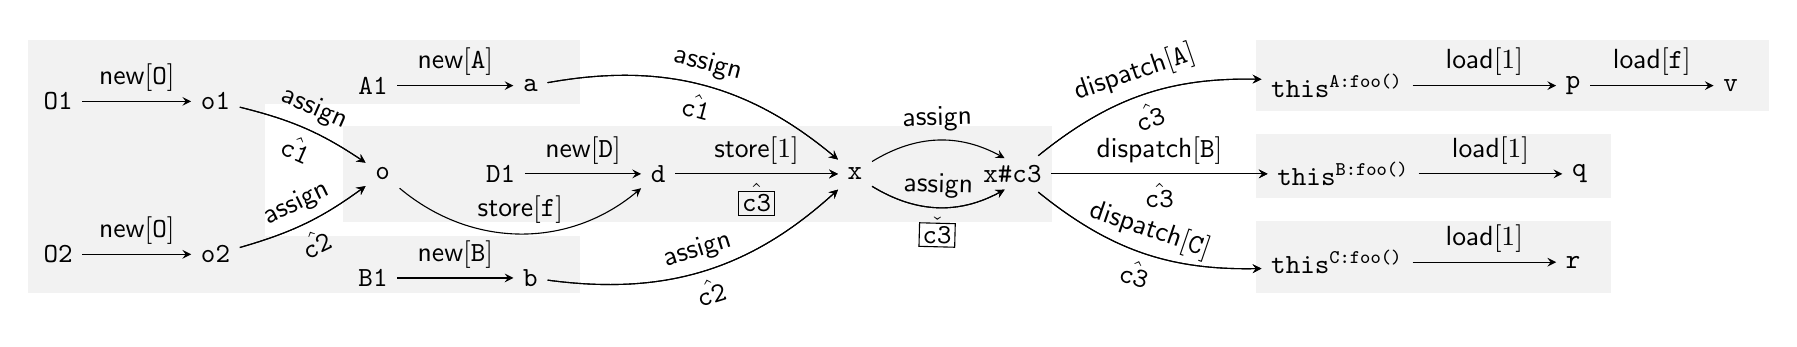
\begin{tikzpicture}
    \draw [draw=black!5, fill=black!5] (5.1,1.7) rectangle (11.6,0.8); % A::foo
    \draw [draw=black!5, fill=black!5] (5.1,0.5,0) rectangle (9.6,-0.3); % B::foo
    \draw [draw=black!5, fill=black!5] (5.1,-0.6,0) rectangle (9.6,-1.5);  % C::foo
    \draw [draw=black!5, fill=black!5] (-10.5,1.7,0) rectangle (-3.5,0.9); % main
    \draw [draw=black!5, fill=black!5] (-10.5,-1.5,0) rectangle (-3.5,-.8); % main
    \draw [draw=black!5, fill=black!5] (-10.5,1.5,0) rectangle (-7.5,-1.3); % main
    \draw [draw=black!5, fill=black!5] (-6.5,0.6,0) rectangle (2.5,-0.6); % bar
    \node(x) {\texttt{x}};
    \node(d)[left of =x, xshift=0.5cm] {\texttt{d}};
    \node(D)[left of=d, xshift=1cm, yshift=.0cm] {\texttt{D1}};
    \node(o)[left of=D, xshift=1.5cm] {\texttt{o}};
    \node(o1)[above left of=o, yshift=-1.2cm] {\texttt{o1}};
    \node(O1)[left of=o1, xshift=1cm] {\texttt{O1}};
    \node(o2)[below left of=o, yshift=1.1cm] {\texttt{o2}};
    \node(O2)[left of=o2, xshift=1cm] {\texttt{O2}};
    \node(xc)[right of=x, xshift=-1cm] {\texttt{x\#c3}};
    \node(a)[above left of=x,yshift=-1cm,xshift=-2cm] {\texttt{a}};
    \node(A)[left of=a, xshift=1cm] {\texttt{A1}};
    \node(b)[below left of=x, yshift=.8cm, xshift=-2cm] {\texttt{b}};
    \node(B)[left of=b, xshift=1cm] {\texttt{B1}};
    \node(thisA)[above right of=xc,xshift=2cm,yshift=-1cm] {$\texttt{this}^\texttt{A:foo()}$};
    \node(p)[right of=thisA]{\texttt{p}};
    \node(v)[right of=p,xshift=-1cm]{\texttt{v}};
    \node(thisB)[right of=xc, yshift=0cm, xshift=1.2cm] {$\texttt{this}^\texttt{B:foo()}$};
    \node(q)[right of=thisB] {\texttt{q}};
    \node(thisC)[below right of=xc, xshift=2cm,yshift=1cm] {$\texttt{this}^\texttt{C:foo()}$};
    \node(r)[right of=thisC]{\texttt{r}};
    
    \path[-stealth]
    (O1) edge[sloped] node{$\new[\texttt{O}]$} (o1)
    (O2) edge[sloped] node{$\new[\texttt{O}]$} (o2)
    
    (A) edge[sloped] node{$\new[\texttt{A}]$} (a)
    (B) edge[sloped] node{$\new[\texttt{B}]$} (b)
    
    (D) edge[sloped, above] node{$\new[\texttt{D}]$} (d)
    
    (a) edge[sloped,bend left=25] node{\assign} (x)
    (a) edge[sloped,bend left=25,below] node{$\hat{\mathtt{c1}}$} (x)
    (o1) edge[sloped,bend left=10] node{\assign} (o)
    (o1) edge[sloped,bend left=10,below] node{$\hat{\mathtt{c1}}$} (o)
    
    (b) edge[sloped,bend right=25] node{\assign} (x)
    (b) edge[sloped,bend right=25,below] node{$\hat{\mathtt{c2}}$} (x)
    (o2) edge[sloped,bend right=10] node{\assign} (o)
    (o2) edge[sloped,bend right=10,below] node{$\hat{\mathtt{c2}}$} (o)
    
    (o) edge[sloped, bend right=40] node{$\store[\texttt{f}]$} (d)
    
    (d) edge[sloped,bend left=0] node{$\store[1]$} (x)
    (d) edge[sloped,bend left=0,below] node{$\hat{\boxed{\mathtt{c3}}}$} (x)
    
    (x) edge[sloped,bend right=30] node{$\assign$} ([shift={(-.1,-.2)}]xc)
    (x) edge[sloped,bend right=30,below] node {$\check{\boxed{\mathtt{c3}}}$} ([shift={(-.1,-.2)}]xc)
%    (x) edge[in=60,out=120,loop,looseness=20] node{$\assign$} (x)
%    (x) edge[in=60,out=120,loop,looseness=20,below] node{$\hat{\boxed{\mathtt{c3}}}$} (x)
    (x) edge[sloped,bend left=30] node{$\assign$} ([shift={(-.1,.2)}]xc)
    
    (xc) edge[sloped,bend left=20] node{$\indispatch[\texttt{A}]$} (thisA)
    (xc) edge[sloped,bend left=20,below] node{$\hat{\mathtt{c3}}$} (thisA)
    (thisA) edge[sloped] node{$\load[1]$} (p)
    (p) edge[sloped] node{$\load[\texttt{f}]$} (v)
    
    (xc) edge[sloped] node{$\indispatch[\texttt{B}]$} (thisB)
    (xc) edge[sloped, below] node{$\hat{\mathtt{c3}}$} (thisB)
    (thisB) edge[sloped] node{$\load[1]$} (q)
    
    (xc) edge[sloped,bend right=20] node{$\indispatch[\texttt{C}]$} (thisC)
    (xc) edge[sloped,bend right=20,below] node{$\hat{\mathtt{c3}}$} (thisC)
    (thisC) edge[sloped] node{$\load[1]$} (r)
    ;
\end{tikzpicture}
}
% \vspace*{-3.5ex}
\caption{The PAG for \LFCR constructed for the program given in \Cref{fig:motivatingExample}.}
\label{fig:pag1}
%\vspace*{-1ex}
\end{figure*}
 
\begin{comment}
We  connect every non-receiver-variable argument  
$a_i$ ($1\leqslant i \leqslant r)$ (under  $\hat{c}$) with
its corresponding parameter $p_i^{m'}$ 
of a method, $m'$,
via  $a_0$ (by CFL-reachability) iff $m'$ is
dispatchable on a receiver object pointed to by $a_0$. 

To relate $a_i$ ($1\leqslant i \leqslant r$) with $a_0$ under 
$\hat{c}$, we will first traverse across a \store edge,
$a_i \xrightarrow[\hat{\boxed{c}}]{\storefield{$i$}} a_0$, i.e., $a_0.i=a_i$ (with the
offset 
$i$ being treated as a special field of $a_0$). We then look for the receiver objects
pointed to by $a_0$. For each receiver object $o$ whose dynamic type is $t$, we will
traverse a path

This is achieved by establishing a path 
 $
 a_i \xrightarrow[\hat{\boxed{c}}]{\storefield{$i$}}a_0 \cdots \xrightarrow{\inew[t]}  \mathtt{o} \xrightarrow{\new[t]} \cdots
a_0 \xrightarrow[\check{\boxed{c}}]{\assign} 
a_0\#\texttt{c} \xrightarrow[\hat{c}]{\indispatch[t]} \texttt{this}^{m'}
\xrightarrow{\loadfield{i}} \mathtt{p}_{i}^{M}
$, such that (1) $a_0$ points to $o$ with its dynamic type being $t$,
(2)
 $\hat{\boxed{c}}$ and $\check{\boxed{c}}$ mark the beginning and end of the CFL-reachability
 traversal for finding the dynamic type $t$,
 (3) $m'$  is dispatched under $\hat{c}$, where $m' = \lookup(\texttt{m}, t)$, and (4) 
 $a_0$ is passed to $p_i^{m'}$ via $a_0.i=a_i$ and $p_i^{m'} = \mathtt{this}.i^{m'}$.

\end{comment}
 




% Note that $\check{\boxed{c}};\hat{c}$ represents two contiguous stack symbols of $L_C$ and must be processed in turn in one transaction. \Cref{subsec:discussion} will discuss how to transform such edges as normal edges with at most one stack symbol as usual.


% Let $L$ be a CFL over $\Sigma$, which is an alphabet drawn  from
% all the edge labels in $G$.
% Each path $p$ in $G$ has a label $L(p)$ in $\Sigma^*$
% formed by concatenating
% in order the labels of the edges in $p$. A node $v$ is \emph{$L$-reachable} from a
% node $u$ if there exists a path $p$ from $u$ to $v$ in $G$, called an \emph{$L$-path}, such
% that $L(p)\in L$.
% To reason about CFL-reachability, we need to traverse the
% edges in $G$ both forwards and backwards.


% For a path $p$ in $G$ such that
% its label is $L(p)=\ell_1,\cdots,\ell_r$ in $L$, the inverse of $p$, i.e.,
% $\overline{p}$ has the label
% $L(\overline{p})=\overline{\ell_r},\cdots,
% \overline{\ell_1}$.



\Cref{fig:pag1} depicts the PAG  used by \LFCR for our motivating example given in ~\Cref{fig:motivatingExample}. As shown, this PAG
(referred to below), which is designed to enable \LFCR to perform
its own built-in on-the-fly call graph construction,
is fundamentally different from the PAG (\Cref{fig:pag2}) used by \manuLFC.

%We will use this PAG for illustration purposes later.



\begin{comment}
For all heap objects, \texttt{A}, \texttt{B}, \texttt{O1}, \texttt{O2} and \texttt{D}, 
a \new edge is added with their respective types being recorded. For static calls, arguments are connected with their corresponding parameters:
$\texttt{a} \xrightarrow[\check{\texttt{c1}}]{\assign} \texttt{x}$,
$\texttt{b} \xrightarrow[\check{\texttt{c2}}]{\assign} \texttt{x}$,
$\texttt{o1} \xrightarrow[\check{\texttt{c1}}]{\assign} \texttt{o}$, and
$\texttt{o2} \xrightarrow[\check{\texttt{c2}}]{\assign} \texttt{o}$.
For the instance calls, all arguments are connected with their corresponding receivers:
$\texttt{x}\xrightarrow[\hat{\boxed{\texttt{c3}}}]{\assign}\texttt{x}$,
$\texttt{d}\xrightarrow[\hat{\boxed{\texttt{c3}}}]{\store[1]}\texttt{x}$, and receivers are connected with their representations at the callsites: 
$\texttt{x} \xrightarrow[\check{\boxed{\mathtt{c3}}}]{\assign} \mathtt{x\#c3}$.
Correspondingly, 
parameters are loaded inside their methods:
% $\texttt{this}^\texttt{A:foo()}\xrightarrow{\load[0]}\texttt{this}^\texttt{A:foo()}$,
$\texttt{this}^\texttt{A:foo()} \xrightarrow{\load[1]}p$,
% $\texttt{this}^\texttt{B:foo()}\xrightarrow{\load[0]}\texttt{this}^\texttt{B:foo()}$,
$\texttt{this}^\texttt{B:foo()}\xrightarrow{\load[1]}q$,
% $\texttt{this}^\texttt{C:foo()}\xrightarrow{\load[0]}\texttt{this}^\texttt{C:foo()}$, 
and
$\texttt{this}^\texttt{C:foo()}\xrightarrow{\load[1]}r$. Finally, dispatch edges are added
between representation of receivers and ``this'' parameter according to different dispatching targets:
$\texttt{x\#c3}\xrightarrow[\hat{\texttt{c3}}]{\indispatch[\mathtt{A}]}\texttt{this}^\texttt{A:foo()}$,
$\texttt{x\#c3}\xrightarrow[ \hat{\texttt{c3}}]{\indispatch[\mathtt{B}]}\texttt{this}^\texttt{B:foo()}$ and
$\texttt{x\#c3}\xrightarrow[\hat{\texttt{c3}}]{\indispatch[\mathtt{C}]}\texttt{this}^\texttt{C:foo()}$.
($\texttt{x\#c3}\xrightarrow[\hat{\texttt{c3}}]{\indispatch[\mathtt{C}]}\texttt{this}^\texttt{C:foo()}$ 
would not be established if PAG is built relying on a context-insensitive pointer analysis.)
\end{comment}


\subsection{\texorpdfstring{\LFCR}{}}
\label{subsec:newCFLs}

%In this section, we present a new CFL-reachability formulation for fully  
%callsite-sensitive and field-sensitive pointer analysis that supports 
%dynamic virtual call dispatching. 

We  express
\LFCR   as the intersection of three CFLs, \capLFCR, 
with each  specifying a
different aspect of \kcs{k}. 
In  \Cref{subsubsec:newLF}, we  introduce \LF,
which describes  field accesses and
dynamic dispatch, for addressing
\challenge{1} and \challenge{2} (\Cref{subsubsec:newLF}). 
\LC, which is given in \Cref{eqn:callsiteLC},  
 enforces callsite-sensitivity by using the
 below-edge terminals $\hat{c}$ and
$\check{c}$
 in the standard manner.
In  \Cref{subsubsec:newLR},
we  introduce \LR (defined over the terminals $\hat{c}$ and
$\check{c}$, $\hat{\boxed{c}}$, and
$\check{\boxed{c}}$), to
  ensure  that parameter passing happens correctly 
in the presence of on-the-fly call
graph construction, for addressing
 \challenge{3}. We shall restrict our discussions to parameter passing  as method
 returns are handled in the same way. 
 When introducing the grammars for \LF and \LR below,
all the double-label \pag edges in a given \pag
are handled in the same way as we have done to \manuLF and \manuLC,
as described in
 \Cref{subsubsec:CFLReachability}.

We shall speak of an \LFC-path as we do for \manuLFC-path (\Cref{subsubsec:manuLFC}). Similarly, we shall
also speak of an \LFCR-path $p$ with the understanding that  
$\LF(p)\in \LF$, 
$\LC(p)\in \LC$, and
$\LR(p)\in \LR$. 

\hl{
To incorporate call graph construction into a CFL-reachability formulation, as defined below, it is necessary to ensure its soundness by guaranteeing that it provides an over-approximation of the set of target methods resolved at a callsite. This means that the constructed call graph should include all possible target methods that could be called at a given callsite. Furthermore, precision is maintained by excluding any spurious target methods from the resolution, ensuring that only relevant and accurate target methods are considered. 
}

\begin{defn}[Soundness and Precision]
\label{def:sound-prec}
Let $L$ be a CFL-reachability formulation that differs from \manuLFC only in
how they handle parameter passing at
virtual callsites, where $L$ itself specifies dynamic method dispatch at virtual callsites
(i.e., performs its 
own built-in
call graph construction) and \manuLFC relies on a separate algorithm $\mathcal{A}$ (by, e.g., calling
\manuLFC recursively to find the receiver objects of virtual callsites under some given contexts)  for performing call graph construction on the fly (Sec.~\ref{sec:LFC+fly}).
Consider a virtual callsite
``$\mathtt{r}.\mathtt{m}(a_1, \dots, a_n); ~ //~ \mathtt{c}$'', where parameter passing  takes place under a given context \CC. Let $T$ be the set of
target methods found by $\mathcal{A}$
at this callsite under $\CC$ (i.e., found also by \manuLFC if a points-to query is issued
for \texttt{r}
for this callsite under $\CC$ separately)
so that \manuLFC can
perform parameter passing for these methods. Then
$L$ is  \emph{sound} if it  enables parameter passing  to be performed
under $\CC$ for at least all
the target methods in $T$ and $L$ is \emph{precise} (in addition to being
sound) if it  enables parameter passing under $\CC$ for exactly the
same target methods in $T$. 
\end{defn}
We shall see that \LFC is  sound (but imprecise) but \LFCR is  precise 
(and obviously  sound).

Let us
consider parameter passing for an argument at a virtual call site
``$\mathtt{r}.\mathtt{m}(a_1, \dots, a_n); ~ // \mathtt{c}$'' 
under a given context $\CC$. In the special case when
 the argument is the receiver variable $\mathtt{r}$, which points  directly to a set of receiver objects, we only need to address \challenge{1} by passing a receiver object
to a target method $m'$ when $m'$ can be dispatched on the receiver object.
If the argument is $a_i$,
the basic idea in addressing
 \challenge{2} and \challenge{3} (facilitated by the PAG designed 
 according to
 the rules given in 
 \Cref{fig:newcflpag})
is to first store  $a_i$  into $\mathtt{r}.i$ (at its special field $i$), then discover the dynamic type $\texttt{t}$ of every receiver object
pointed to by $\mathtt{r}$ under $\CC$ and propagate $\texttt{t}$ to the callsite \texttt{c} where $ \mathtt{m'} = \lookup(\texttt{m}, \texttt{t})$,
and finally, assign
$\texttt{this}^{\mathtt{m}'}.i$ to $p_i^{\mathtt{m}'}$ for this callsite under
still the same given context \CC. As discussed earlier, method returns are
handled similarly.

\begin{comment}
Let \manuLFCDD be the demand-driven formulation of \manuLFC for solving \kcs{k}
by using a
separate algorithm for on-the-fly construction under the assumption that
it can handle parameter passing for receiver variables correctly (without
suffering from the precision loss discussed in Sec.~\ref{sec:LFC+fly}). 
\LFCR is designed to solve \kcs{k}  with CFL-reachability fully  by computing the same points-to information as \manuLFCDD.
Consider our motivating example in \Cref{fig:motivatingExample}.
As discussed in Sec.~\ref{sec:LFC+fly}, \manuLFCDD will assert that \texttt{v} 
points to
 \commentfont{O1} only due to the
existence of the  \manuLFC-path  in \Cref{eq:LFCPathCGPreciseI}.
\end{comment}

\begin{comment}
With \LFCR, we will reach the same conclusion  according
to the \LFCR-path:

Consider our motivating example in \Cref{fig:motivatingExample}.
With \manuLFC \cite{sridharan2006refinement}, as discussed in \Cref{subsubsec:manuLFC}, \texttt{v} is found to point to
both \commentfont{O1} and \commentfont{O2} if the graph is pre-built (due to the
existence of the two \manuLFC-paths given in \Cref{eq:LFCPathCGPreciseI} and
\Cref{eq:LFCPathCGPreciseII})
and \commentfont{O1}  only if the call graph is built on the fly.
With \LFCR, \texttt{v} is found to point to \commentfont{O1}  only according
to the following path:

{
\setlength{\abovedisplayskip}{.8ex}
\setlength{\belowdisplayskip}{.8ex}
\begin{equation}
  \centering
\label{eq:ex-patho1-to-v}
\begin{tabular}{l} 
% \footnotesize
\vspace*{1ex}
\commentfont{O1}$\xrightarrow{\new[\texttt{O}]}
\texttt{o1}\xrightarrow[\hat{\mathtt{c1}}]{\assign}
\texttt{o} \xrightarrow{\storefield{f}} \texttt{d}
\xrightarrow{\inewfield{\texttt{D}}}$ \commentfont{D1} 
$\xrightarrow{\new[\texttt{D}]} 
\texttt{d}$ $\xrightarrow[\hat{\boxed{\texttt{c3}}}]{\store[1]}\texttt{x}\xrightarrow[\check{\texttt{c1}}]{\iassign}\texttt{a} $ $\xrightarrow{\inewfield{\texttt{A}}}$\commentfont{A1} \\[3ex]
\begin{tikzpicture}[-, remember picture,overlay]
\def\lx{11.5}\def\ly{1.2}
\def\dy{.68}\def\ny{.07}
\draw(\lx, \ly) -- (\lx+.1, \ly) -- (\lx+.1, \dy);
\draw[dashed] (\lx+.1, \dy) -- (-.12,\dy);
\draw(-.12,\dy) -- (-.12, \ny);
\draw[->] (-.12, \ny) -- (0.06, \ny);
\end{tikzpicture}
% \footnotesize 
$\xrightarrow{\new[\texttt{A}]}\texttt{a}\xrightarrow[\hat{\texttt{c1}}]{\assign}\texttt{x} \xrightarrow[\check{\boxed{\texttt{c3}}}]{\assign} \texttt{x\#c3}$ $\xrightarrow[\hat{\texttt{c3}}]{\indispatch[\texttt{A}]}\texttt{this}^\texttt{A:foo()}
\xrightarrow{\load[1]}\texttt{p}
    \xrightarrow{\load[\texttt{f}]} \texttt{v}$ \\[3ex]
% \begin{tikzpicture}[-, remember picture,overlay]
% \def\lx{7.1}\def\ly{.95}
% \def\dy{.45}\def\ny{.068}
% \draw(\lx, \ly) -- (\lx+.1, \ly) -- (\lx+.1, \dy);
% \draw[dashed] (\lx+.1, \dy) -- (-.12,\dy);
% \draw(-.12,\dy) -- (-.12, \ny);
% \draw[->] (-.12, \ny) -- (0.06, \ny);
% \end{tikzpicture}
% \footnotesize 
% $\xrightarrow[\hat{\texttt{c3}}]{\indispatch[\texttt{A}]}\texttt{this}^\texttt{A:foo()}
% \xrightarrow{\load[1]}\texttt{p}
%     \xrightarrow{\load[\texttt{f}]} \texttt{v}$
\end{tabular}
\end{equation}
}
\hspace*{-1.1ex}
\end{comment}


Let us revisit our motivating example with its PAG depicted in
\Cref{fig:pag1}. With \LFCR, we will ensure that the PAG contains a unique
\LFCR-path from \commentfont{O1} to \texttt{v}, as depicted in 
\Cref{eq:ex-patho1-to-v}, so that \texttt{v} can point to 
\commentfont{O1}  only when \texttt{bar()} is called at callsite \texttt{c1}. 
The sub-path from \commentfont{O1} to
\texttt{d} indicates that \commentfont{O1} is stored into \texttt{d.f}, where
\texttt{d} points to \commentfont{D1}, due to the call 
``\inline{bar(a, o1); // c1}''. The sub-path from \texttt{d} to \texttt{p}
reveals parameter passing from \texttt{d} to \texttt{p} at 
``\inline{x.foo(d); // c3}'' for the target
method \texttt{A:foo()} discovered on the fly by \LFCR itself under $\CC=[\texttt{c1}]$. In 
\Cref{subsubsec:challenges},  we have already discussed how we
address \challenge{1} -- \challenge{3} at this callsite. We wish to add
now that $\hat{\boxed{\texttt{c3}}}$ and $\check{\boxed{\texttt{c3}}}$ mark
the beginning and end of dynamic dispatch performed at this callsite for
\texttt{d}, respectively. During the CFL-reachability traversal
between $\hat{\boxed{\texttt{c3}}}$ and $\check{\boxed{\texttt{c3}}}$, we
discover that
\texttt{x} points to \commentfont{A1}   of  type \texttt{A}
 under [\texttt{c1}] must return to \texttt{x} under also [\texttt{c1}].
%(requiring $\hat{{\texttt{c1}}}$ to be matched by $\check{{\texttt{c1}}}$), .
Given the receiver object \commentfont{A1} found,
we can then
dispatch \texttt{A:foo()} via $\texttt{x\#c3}$  $\xrightarrow[\hat{\texttt{c3}}]{\indispatch[\texttt{A}]}\texttt{this}^\texttt{A:foo()}$
so that \texttt{d} can be passed to \texttt{p} 
under $[\texttt{c3}, \texttt{c1}]$, with
  \texttt{c3}  recovered from ${\boxed{\texttt{c3}}}$. While \manuLFC \cite{sridharan2006refinement} uses
  [\texttt{c3}]  for 
 passing \texttt{d} to \texttt{p}  
  (\Cref{eq:LFCPathCGPreciseI}), \LFCR uses
  $[\texttt{c3}, \texttt{c1}]$ more specifically
 %(with  $[\hat{\texttt{c1}}]$ and   $[\check{\texttt{c1}}]$ being matched)
   to indicate that this happens only when \texttt{x} points to \commentfont{A1}  under [\texttt{c1}].




% and \challenge{5} (\Cref{subsubsec:newLX}) 


%We no longer introduce \LC as it is exactly same as \manuLC but just remind that symbols $\hat{\boxed{c}}$ and $\check{\boxed{c}}$ in below edges are not terminals of \LC.

% We sometimes use superscripts $O$ and $N$ (e.g., $L_{F}^{O}$ and $L_{F}^{N}$) to differentiate the grammars defined in the traditional formulation and our new formulation. We drop the superscript where the context is clear. 

% \begin{itemize}
% \item $L_F$ ensures that \kcs{k} performs a field-sensitive pointer analysis with call graph built on the fly context-insensitively. 
% \item $L_C$ ensures that 
% \kcs{k} is callsite-sensitive by not only matching method calls and returns as a balanced-parentheses problem but also ensures context is restored when dispatching.  
% \end{itemize}

\subsubsection{The \LF Language}
\label{subsubsec:newLF}

% A CFL-Reachability Formulation of call-site based pointer analysis
% We will define a language, $L_{FC}$, over $\Sigma$
% so that \kcs{k} can be solved by reasoning about CFL-reachability 
% in $G_{\pag}$. For convenience, 
% we will express $L_{FC}$ as the intersection of two 
% balanced-parentheses CFLs,
% $L_{FC} = L_F \cap L_C$, with the two languages specifying two different
% aspects of \kcs{k} as shown below.
% As a result, determining if
% a variable $v$ points to an object $O$ requires finding a path $p$ between the nodes $v$ and $O$ in $G$ such that 
% $L_{F}(p)\in L_{F}$ and $L_{C}(p)\in L_{C}$:



 
This CFL
describes not only field-sensitive accesses as balanced parentheses as in \manuLF given in \Cref{eqn:callsiteLF} but also
dynamic dispatch in the language itself:
%{
% \begin{equation}
% \label{eqn:newLF}
% \tiny
% \begin{split} 
% \flowsto & \longrightarrow \new ~ \flows^* \\
% \iflowsto & \longrightarrow \iflows^* ~ \inew \\
% \flows & \longrightarrow \assign \mid  \storefield{f} \ \alias \ \loadfield{f} \mid \dispatch\\
% \iflows & \longrightarrow \iassign \mid \iloadfield{f}\ \alias \ \istorefield{f} \mid \idispatch \\
% \alias & \longrightarrow \iflowsto\ \flowsto \\
% \dispatch & \longrightarrow \storefield{i} \ \iflowsto \ \typefound[t] \ \flowsto \ \indispatch[t] \ \loadfield{i} \\
%             & \longrightarrow \storefield{ret} \ \iindispatch[t] \ \iflowsto \ \itypefound[t] \ \flowsto \ \loadfield{ret}  \\ 
% \idispatch & \longrightarrow \iloadfield{i} \ \iindispatch[t] \ \iflowsto \ \itypefound[t] \ \flowsto \ \istorefield{i}  \\
%             & \longrightarrow \iloadfield{ret} \ \iflowsto \ \typefound[t] \ \flowsto \ \indispatch[t] \ \istorefield{ret} 
% \end{split}
% \end{equation}
\begin{equation} 
% \footnotesize
\label{eqn:finalNewLF}
\begin{tabular}{rcl}
$\flowsto$ & $\longrightarrow$ & $\new[\texttt{t}]~(\flows~|~\indispatch[\texttt{t}])^*$ \\[1ex]
$\flows$ & $\longrightarrow$ & $\assign \mid \store[\texttt{f}] \ \alias \ \load[\texttt{f}]$\\[1ex] % \mid \store[i] \ \alias \ \load[i] \\
$\alias$ & $\longrightarrow$ & $\iflowsto ~ \flowsto$ \\[1ex]
$\iflowsto$ & $\longrightarrow$ & $(\iindispatchfield{t}~|~\iflows)^*~\inewfield{\texttt{t}}$ \\[1ex]
$\iflows$ & $\longrightarrow$ & $\iassign \mid \iloadfield{\texttt{f}} \ \alias \ \istorefield{\texttt{f}}$ \\[1ex] %\mid \iloadfield{i} \ \alias \ \istorefield{i} \\
\end{tabular}
\end{equation}
%}
%\noindent
%where the set of terminals includes all the edge labels
% (of both regular edges and their inverses) in the \pag. 
\begin{comment}
If $O\; \flowsto\; v$,  then $v$ is
\LF-reachable from $O$, i.e., $O$ flows to $v$, implying that $v$ points to $O$.
In fact, $\iflowsto$ is the inverse of the $\flowsto$ relation, representing
the standard points-to relation. Thus,
if $v\; \iflowsto\; O$,  then $v$ points to $O$.
Note that $\iflows$ is  also the
inverse of \flows. When computing the points-to information, we need
to traverse the edges in \pag forwards to establish \flowsto and
\flows and also backwards to establish $\iflowsto$ and $\iflows$, with both
performed recursively (due to the need for resolving the aliases in the
program).
\end{comment}

All the below-edge
labels are handled similarly as in the case of \manuLF. By
decomposing each double-label edge into
two single-label edges as described in
\Cref{subsubsec:CFLReachability}, $\flows$ becomes
$\flows \longrightarrow ... \mid \hat{c} \mid \check{c} \mid
\hat{\boxed{c}} \mid \check{\boxed{c}}  $  and
$\iflows$ becomes
$\iflows \longrightarrow ... \mid \hat{c} \mid \check{c} \mid
\hat{\boxed{c}} \mid \check{\boxed{c}}  $ 
in their full generality.

In designing \LF, we have extended 
\manuLF~\cite{sridharan2005demand, sridharan2006refinement} by
preserving its capability in handling field accesses as balanced parentheses
and adding a new capability in supporting dynamic dispatch, and consequently, on-the-fly
call graph construction. Below we describe separately how \LF is designed to 
address \challenge{1} and \challenge{2} and why we have selected
such a dynamic dispatch approach.
%The key novelty in addressing  \challenge{1} -- \challenge{3} is to propagate the type information of a receiver object to where  dynamic dispatch is triggered by parameter passing.
 
\begin{comment}
Given a virtual 
callsite
$\mathtt{x = } ~ a_0.\mathtt{m}(a_1,..., a_r)$,
the key novelty in addressing
 \challenge{1} and \challenge{2} (facilitated by the PAG designed according to
 the rules given in 
 \Cref{fig:newcflpag})
is to first store  $a_i$ ($1\leqslant i
\leqslant r$)  into $a_0.i$, then discover the dynamic type $t$ of every receiver object
pointed by $a_0$ and propagate $t$ to this callsite  (and others invoked on
$\texttt{this}^{m'}$ in $m'$) in terms of
 $\new[t]~(\flows~|\linebreak \indispatch[t])^*$,  where $ m' = \lookup(\texttt{m}, t)$,
and finally, retrieve $a_i$ (available now in
$\texttt{this}^{m'}.i$) and pass it to $p_i^{m'}$.
\end{comment}

%By construction, arguments-parameter pairing (\texttt{store[i]} matched by \texttt{load[i]}), and dispatching type checking (\texttt{new[t]} checked by \texttt{dispatch[t]}).

%In the case of \flows, \store\![i] \ \alias \ \load\![i] represents the value flow from an argument to its corresponding formal parameter or from a return value to a return target.




% \subsubsection{$L_X$}
% \label{subsubsec:newLX}

\paragraph{\challenge{1} \label{paragraph:chl1} } In addressing this first challenge concerning parameter passing 
at a virtual callsite, we
must distinguish its receiver variable from its other arguments to ensure that 
the receiver objects pointed by the receiver variable can only be passed to the \texttt{this} variable of 
a method  that can be dispatched on these receiver objects. Consider 
\inline{x.foo(null)} in the code snippet given  in ~\Cref{fig:recvobj}, where \texttt{x}
may point to both \commentfont{A1} and \commentfont{B1}. The traditional \manuLFC-based
formulation that uses a separate algorithm for call graph construction  (\Cref{fig:manucflpag}) will 
end up passing  both \commentfont{A1} and \commentfont{B1} to 
$\texttt{this}^{\texttt{A:foo()}}$ due to the existence of the two \manuLFC-paths given in
 \Cref{eq:LFCPathCGOnFlyI} and \Cref{eq:LFCPathCGOnFlyII}, 
although \commentfont{B1} is spurious (\Cref{rule:cfapta}).



% For receiver objects, they could only be dispatched to target methods that are compatible with %their own types, which, however, is not reflected by \manuLFC. %In order to achieve this goal, we must use a stack to record the type information of the current value flow. 

In  \LF, we make explicit the dynamic types of  objects 
in the  four kinds of terminals, $\new[\texttt{t}]$, $\inewfield{\texttt{t}}$, $\indispatch[\texttt{t}]$, and $\iindispatchfield{\texttt{t}}$. During a
 $\flowsto$ ($\iflowsto$) traversal, we require the type information in 
 $\indispatch[\texttt{t}]$ ($\iindispatchfield{\texttt{t}}$) to be consistent with that in
 its corresponding $\new[\texttt{t}]$ ($\inewfield{\texttt{t}}$). As a result, the two
 \manuLFC-paths in \Cref{eq:LFCPathCGOnFlyI} and \Cref{eq:LFCPathCGOnFlyII} become:
\begin{equation*} 
% \scriptsize
  \centering
\label{eq:newLFCPathCGOnFlyI}
\begin{tabular}{@{\hspace{.5ex}}l} 
\commentfont{A1}$\xrightarrow{\new[\texttt{A}]}  \texttt{a} \xrightarrow{\store[\texttt{f}]} \texttt{d}
\xrightarrow{\inewfield{\texttt{D}}}$ \commentfont{D1} 
$ \xrightarrow{\new[\texttt{D}]} \texttt{d}
\xrightarrow{\load[\texttt{f}]} \texttt{x} \xrightarrow{\assign}\texttt{x\#c}
\xrightarrow[\hat{\mathtt{c}}]{\indispatch[\texttt{A}]} \mathtt{this}^{\texttt{A:foo()}}$
\end{tabular}
% \vspace{-2ex}
\end{equation*}
\begin{equation*} 
% \scriptsize
  \centering
\label{eq:newLFCPathCGOnFlyII}
\begin{tabular}{@{\hspace{.5ex}}l} 
\commentfont{B1}$\xrightarrow{\new[\texttt{B}]} \texttt{b} \xrightarrow{\store[\texttt{f}]} \texttt{d}
\xrightarrow{\inewfield{\texttt{D}}}$ \commentfont{D1} 
$ \xrightarrow{\new[\texttt{D}]} \texttt{d}
\xrightarrow{\load[\texttt{f}]} \texttt{x} \xrightarrow{\assign}\texttt{x\#c} 
\xrightarrow[\hat{\mathtt{c}}]{\indispatch[\texttt{A}]} \mathtt{this}^{\texttt{A:foo()}}$
\end{tabular}
\end{equation*}
The first is an \LF-path since $\new[\texttt{A}] ~ \flows^* ~ \indispatch[\texttt{A}] \in \mbox{\LF}$,
but the second is not an \LF-path since 
 $\new[\texttt{B}] ~ \flows^* ~ \indispatch[\texttt{A}] \notin \mbox{\LF}$. Thus,
  \commentfont{B1} cannot flow to $\mathtt{this}^{\texttt{A:foo()}}$ spuriously.

In
\Cref{eq:ex-patho1-to-v}, \commentfont{A1} can be passed to 
$\texttt{this}^\texttt{A:foo()}$ since \texttt{A:foo()} can be dispatched
on \commentfont{A1}.


\begin{lem}
\label{theorem:handlingReceiver}
Consider a virtual callsite $\mathtt{x = } ~ \mathtt{r}.\mathtt{m}(a_1, \dots, a_n)$ in Java. 
In \LF,
every receiver object pointed to by $\mathtt{r}$  flows only to the \texttt{this} variable of a method that can be dispatched on the receiver object.
%let $m'$ be a resolved target method and $O$ be a receiver object (i.e, $O \in \cipointsto{a_0})$ of \texttt{c}, then $O \in \cipointsto{\texttt{this}^{m'}}$ only if $\texttt{this}^{m'}$ is \LF-reachable from $O$.
\end{lem}
\begin{proof}[Proof Sketch]
Follows from the definition of \LF.
%\LF requires the type of an object pointed to by $\mathtt{r}$ to be 
%used for dynamic dispatch at the virtual callsite.
%($a_0 \xrightarrow{\indispatch[t]} \texttt{this}^{m'}$) 
%to be the same as in $O \xrightarrow{\new[t]} \cdots a_0$ to be consistent with that  in . 
\end{proof}




\begin{comment}
\Cref{fig:adaptedNewcflpag} shows the adapted \pag construction rules with changes being highlighted in \textcolor{blue}{blue}. We also encode the type information by adding symbols such as $\hat{\boxed{t}}$ and  $\check{\boxed{t}}$ to the below-edges of \pag. 

\begin{figure}[htbp]
\begin{center}
\begin{adjustbox}{width=\linewidth}
\begin{tabular}{c}
			\ruledef{
				 \mathtt{x = \mathsf{\mathbf{new}} ~ T} ~ { \mathtt{//~o}} \rulespace t = \typeof(\mathtt{o})
			}{
				\mathtt{o} \xrightarrow[{\color{blue}\hat{\boxed{t}}}]{\new} \mathtt{x} \rulespace
				\mathtt{o} \xrightarrow[\tau]{\typefound[t]} \mathtt{o}
			}
		 \rulename{New} 
		 \quad
			\ruledef{
			    \mathtt{x = y} 
			}{
				\mathtt{y} \xrightarrow{\assign} \mathtt{x}
			}
			\rulename{Assign}
			\\ [5ex]
	 		\ruledef{
            			    \mathtt{x = y.f} 
            			    \rulespace { \color{blue} t <: \typeof(\texttt{y}) }
            			}{
            				\mathtt{y} \xrightarrow[{\color{blue} \check{\boxed{t}}}]{\loadfield{f}} \mathtt{x}
            			}
        
        	 \rulename{Load}
        	 \quad
			\ruledef{
			    \mathtt{x.f = y} 
			    \rulespace { \color{blue} t <: \typeof(\texttt{x}) }
			}{
				\mathtt{y} \xrightarrow[{\color{blue} \hat{\boxed{t}} }]{\storefield{f}} \mathtt{x} 
			}
			 \rulename{Store}
             \\[5ex]
            	\ruledef{
            			    \mathtt{p} ~ \text{is the } ~ i \text{-th parameter of }~ \texttt{m} ~ (i > 0)
            			    \rulespace { \color{blue} t <: \typeof(\texttt{this}^{\texttt{m}}) }
            			}{
            							\mathtt{this}^{\texttt{m}} \xrightarrow[{\color{blue} \check{\boxed{t}}}]{\loadfield{i}} \mathtt{p} 
            			}
        
        	 \rulename{Param}
        	 \\[5ex]
        % 	 \quad
			\ruledef{
		    \mathtt{r} ~ \text{is the return variable of } ~ \texttt{m}
		    \rulespace { \color{blue} t <: \typeof(\texttt{this}^\texttt{m}) }
			}{
				\mathtt{r}  \xrightarrow[{\color{blue} \hat{\boxed{t}}}]{\storefield{ret}} \mathtt{this}^{\texttt{m}}
			}
			 \rulename{Return}
             \\[5ex]
			\ruledef{
			   \mathtt{x = } ~ a_0.\mathtt{m}(a_1,..., a_r) ~ \mathtt{//~ c} 
			 %  \rulespace o \in \cipointsto{a_0} 
			   \rulespace t <: \typeof(a_0)
			   \rulespace m' = \lookup(\texttt{m}, t) 
			}{
			\rulespace \forall \ i \in [{\color{blue} 1}, r]: a_i \xrightarrow[\hat{\boxed{c}} \ {\color{blue} \hat{\boxed{t}}} ]{\storefield{$i$}} a_0
			\rulespace a_0 \xrightarrow[\check{\boxed{c}} \ {\color{blue} \hat{\boxed{t}}}]{\loadfield{$\texttt{ret}$}} \mathtt{x}
			\rulespace {\color{blue}  a_0 \xrightarrow[\hat{\boxed{c}}]{\assign} a_0 }
            \rulespace a_0 \xrightarrow[\check{\boxed{c}};\hat{c} \ {\color{blue} \check{\boxed{t}};\hat{\boxed{t}}} ]{\indispatch[t]} p_0^{m'} 
			}
			\rulename{Call}
		\end{tabular}
	\end{adjustbox}
	\end{center}
	\caption{The adapted PAG construction rules from \Cref{fig:newcflpag} for supporting dynamic dispatching for receiver objects in our new CFL-reachability formulation. The inverse edges are omitted. Changes are highlighted in \textcolor{blue}{blue}.}
	\label{fig:adaptedNewcflpag}
\end{figure}

To record the type information of current value flow, we add an additional 
CFL grammar $L_X$ which is defined below:
\begin{equation}
\label{eqn:callsiteLX}
\footnotesize
    \begin{split}
L_X  & \longrightarrow  \textsf{Exit} ~ \textsf{Entry} \\
\textsf{Exit}  & \longrightarrow \textsf{Exit} ~ \textsf{xbalance} \mid \textsf{Exit} \ \check{\boxed{t}} \mid \epsilon \\ 
\textsf{Entry}  & \longrightarrow \textsf{Entry} ~ \textsf{xbalance} \mid \textsf{Entry} \ \hat{\boxed{t}} \mid \epsilon \\
\textsf{xbalance} & \longrightarrow \textsf{xbalance} ~ \textsf{xbalance} \mid \hat{\boxed{t}} ~ \textsf{xbalance} ~ \check{\boxed{t}} \mid \epsilon
    \end{split}
\end{equation}

With $L_X$, the top element in $L_X$ stack during the computation of pointer analysis always reflects the type information of current value flow. 
\end{comment}


\begin{comment}
Below, we show that $L_X$ and $L_F$ can be merged as a single CFL by encoding type information also into $L_F$ stack in an appropriate order.

\Cref{fig:finalNewcflpag} gives the final \pag construction rules. Comparing with \Cref{fig:adaptedNewcflpag}, we could find that type symbols in the below edges have been moved to the above edges. The \typefound[t] edges have 
been removed as the type information they contains have been expressed in $\new[t]$ and $\inew[t]$. Similarly, 
${\color{blue} \check{\boxed{t}};\hat{\boxed{t}}}$ has been directly removed as \indispatch[t] has already contained the type information. 
\end{comment}


% The final $L_F$ grammar is defined in \Cref{eqn:finalNewLF}. In this grammar, we require that $\store[\texttt{f}][t]$
% match with $\load[t][\texttt{f}]$, $\store[\texttt{i}][t]$ match with $\load[t][\texttt{i}]$, and $\new[t]$ match with $\indispatch[t]$. 

% \begin{equation} \tiny
% \label{eqn:finalNewLF}
% \begin{split}
% \flowsto & \longrightarrow \new[t]~(\flows~|~\indispatch[t])^*\\
% \iflowsto & \longrightarrow (\iindispatch[t]~|~\iflows)^*~\inew[t]\\
% \flows & \longrightarrow \assign\\&\qquad|~\store[\texttt{f}][t] \ (\iindispatch[t]~|~\iflows)^*\inew[t]~\new[t]~(\flows~|~\indispatch[t])^* \ \load[t][\texttt{f}]\\&\qquad|~\store[i][t] \ (\iindispatch[t]~|~\iflows)^*\inew[t]~\new[t]~(\flows~|~\indispatch[t])^* \ \load[t][i]\\
% \iflows & \longrightarrow \iassign\\&\qquad|~\iload[\texttt{f}][t] \ (\iindispatch[t]~|~\iflows)^*\inew[t]~\new[t]~(\flows~|~\indispatch[t])^* \ \istore[t][\texttt{f}]\\&\qquad|~\iloadfield{i}[t] \ (\iindispatch[t]~|~\iflows)^*\inew[t]~\new[t]~(\flows~|~\indispatch[t])^* \ \istore[t][i]\\
% \end{split}
% \end{equation}


% \subsection{Discussion}
% \label{subsec:discussion}





\begin{comment}
i.e., associating the value flow of arguments with that of receiver variables, by enforcing the value flows from arguments (return values) to their corresponding receiver variables with specially designed \pag edges, i.e., \store[i] and \load[\texttt{ret}], added via \rulename{C-VCall}. Generally, dynamic dispatching values from an argument $a_i$ to a formal parameter $p_i^{m'}$ dependents on $t$ (the dynamic types of the receiver objects), $\texttt{m}$ (the signature of the invoking method), and $i$ (the identifier of the argument it self).   While the later two could be obtained at hand at a callsite, the receiver objects and the receiver variable $a_0$ could be further apart in the program, separated by a long sequence of method calls (with complex field accesses). 
\end{comment}

\paragraph{\challenge{2} \label{paragraph:chl2}} In addressing this second  challenge, we must decide
how to trigger dynamic dispatch during the course of 
parameter passing at a virtual callsite.  We accomplish this by using
\capLFC. To understand our approach, we examine again the \LFCR-path given in
\Cref{eq:ex-patho1-to-v}. For convenience, we duplicate it below
by ignoring $\hat{\boxed{\texttt{c3}}}$ and 
$\check{\boxed{\texttt{c3}}}$ to obtain the following
\LFC-path:

{
\setlength{\abovedisplayskip}{.8ex}
\setlength{\belowdisplayskip}{.8ex}
\begin{equation}
  \centering
\label{eq:ex-patho1-to-v-duplicate}
\begin{tabular}{l} 
% \footnotesize
\vspace*{1ex}
\commentfont{O1}$\xrightarrow{\new[\texttt{O}]}
\texttt{o1}\xrightarrow[\hat{\mathtt{c1}}]{\assign}
\texttt{o} \xrightarrow{\storefield{f}} \texttt{d}
\xrightarrow{\inewfield{\texttt{D}}}$ \commentfont{D1} 
$\xrightarrow{\new[\texttt{D}]} 
\texttt{d}$ $\xrightarrow{\store[1]}\texttt{x}\xrightarrow[\check{\texttt{c1}}]{\iassign}\texttt{a} $ $\xrightarrow{\inewfield{\texttt{A}}}$\commentfont{A1} \\[5ex]
\begin{tikzpicture}[-, remember picture,overlay]
\def\lx{11.5}\def\ly{1.5}
\def\dy{.85}\def\ny{.07}
\draw(\lx, \ly) -- (\lx+.1, \ly) -- (\lx+.1, \dy);
\draw[dashed] (\lx+.1, \dy) -- (-.12,\dy);
\draw(-.12,\dy) -- (-.12, \ny);
\draw[->] (-.12, \ny) -- (0.06, \ny);
\end{tikzpicture}
% \footnotesize 
$\xrightarrow{\new[\texttt{A}]}\texttt{a}\xrightarrow[\hat{\texttt{c1}}]{\assign}\texttt{x} \xrightarrow{\assign} \texttt{x\#c3}$ $\xrightarrow[\hat{\texttt{c3}}]{\indispatch[\texttt{A}]}\texttt{this}^\texttt{A:foo()}
\xrightarrow{\load[1]}\texttt{p}
    \xrightarrow{\load[\texttt{f}]} \texttt{v}$ \\[3ex]
% \begin{tikzpicture}[-, remember picture,overlay]
% \def\lx{7.1}\def\ly{.95}
% \def\dy{.45}\def\ny{.068}
% \draw(\lx, \ly) -- (\lx+.1, \ly) -- (\lx+.1, \dy);
% \draw[dashed] (\lx+.1, \dy) -- (-.12,\dy);
% \draw(-.12,\dy) -- (-.12, \ny);
% \draw[->] (-.12, \ny) -- (0.06, \ny);
% \end{tikzpicture}
% \footnotesize 
% $\xrightarrow[\hat{\texttt{c3}}]{\indispatch[\texttt{A}]}\texttt{this}^\texttt{A:foo()}
% \xrightarrow{\load[1]}\texttt{p}
%     \xrightarrow{\load[\texttt{f}]} \texttt{v}$
\end{tabular}
\end{equation}
}
\hspace*{-1.1ex}


To find whether \commentfont{O1} can flow into \texttt{v} starting from 
``\inline{bar(a,o1); // c1}'', we need to perform parameter passing
for \texttt{d} at ``\inline{x.foo(d); // c3}'' under context
$\CC=[\texttt{c1}]$. This is achieved 
by traversing the  sub-path   from  \texttt{d} to
 the parameter \texttt{p} of \texttt{A:foo()}.  
We start with 
a store 
$\texttt{d}\xrightarrow{\store[1]}\texttt{x}$
to trigger a 
 $\iflowsto$ traversal via
$\texttt{x} \xrightarrow[\check{\texttt{c1}}]{\iassign}\texttt{a} \xrightarrow{\inewfield{\texttt{A}}}$\commentfont{A1} 
 under the given context $\CC=[\texttt{c1}]$,
return to \texttt{x}  backwards via
\commentfont{A1}
$\xrightarrow{\new[\texttt{A}]} \texttt{a}
\xrightarrow[\hat{\texttt{c1}}] {\assign} \texttt{x}$, dispatch at the callsite
via $
\texttt{x}
\xrightarrow{\assign} \texttt{x\#c3} \xrightarrow[\hat{\texttt{c3}}]{\indispatch[\texttt{A}]} 
\texttt{this}^{\texttt{A:foo()}} $, and finally, pass \texttt{d} to 
\texttt{p} via a load
$\texttt{this}^\texttt{A:foo()}
\xrightarrow{\load[1]}\texttt{p}$.
While \manuLFC passes \texttt{d} to \texttt{p}
in 
\Cref{eq:LFCPathCGPreciseI} by one  \assign edge $d\xrightarrow[\hat{{\mathtt{c3}}}]{\assign} \mathtt{p}$ under [\texttt{c3}],
\LFC passes 
\texttt{d}    to \texttt{p}  via a sequence of PAG edges  under [\texttt{c3},\texttt{c1}] (indicating
that this parameter passing happens only when \texttt{x} point to
\commentfont{A1} under  [\texttt{c1}]).

According to \Cref{def:sound-prec}, \LFC is sound if it can perform parameter passing
for a superset of 
the set of target methods that can be possibly dispatched at a virtual callsite.

\begin{lem}
\label{thm:lfc-imprecise}
\LFC is sound  in handling parameter passing at every virtual
callsite.
\end{lem}
\begin{proof}[Proof Sketch]
Let 
``$\mathtt{r}.\mathtt{m}(a_1, \dots, a_n); ~ // ~ \mathtt{c}$''
be  a fixed but arbitrary virtual callsite, where parameter passing for
one of its arguments takes place under a given context \CC. Let $T$ be the set of
target methods found on the fly at this callsite under $\CC$ by a separate call graph
construction algorithm used in \manuLFC. As \texttt{r} is handled
similarly as in \manuLFC, it suffices to consider parameter passing for a non-receiver-variable argument
$a_i$. Due to the existence of $a_i \xrightarrow{\store[i]} \mathtt{r}$, \LFC will perform dynamic dispatch by finding the receiver
objects pointed to by \texttt{r} under also  \CC.
As \LFC differs from \manuLFC only in their handling of parameter passing 
at virtual callsites, the set of target methods found by \LFC must include
$T$. In addition, for every target  $m' \in T$, there  always exists
a path $q$ in the PAG:
\begin{equation}
    \label{eq:proof-valid-DP}
a_i \xrightarrow{\store[i]} \mathtt{r} ~
\iflowsto ~ O ~ \flowsto ~\mathtt{r}
 \xrightarrow{\assign} \mathtt{r}\#c
 \xrightarrow[\hat{c}]{\indispatch[\texttt{\_}]}\texttt{this}^{m'}
 \xrightarrow{\load[i]} p_i 
 \end{equation}
 where $p_i$ is the $i$-th parameter of $m'$.
 Here, if we write $u$ to represent the $\overline{\flowsto}$-path ``$\mathtt{r} ~
\iflowsto ~ O$'', then the \flows-path ``$O ~ \flowsto ~\mathtt{r}$'' is its
inverse $\overline{u}$. By construction, $a_i ~\flows~ p_i$ according to $\LF$ and
$\LC(q) \in \LC$ according to \LC. In addition,
$\LC(q)$ is guaranteed to be a sequence of (calling) contexts that can happen
under $\CC$ since $u$ is traversed under \CC. Therefore, \LFC is sound by Definition~\ref{def:sound-prec}.
\begin{comment}
In terms of their PAGs used, 
\LFCR differs from \manuLFCDD (i.e., \manuLFC) only in how virtual callsites are handled.
Given a program, its PAG  used by \LFC (\Cref{fig:newcflpag}), together with
\LF, ensures that for every virtual callsite $\mathtt{x} = \mathtt{r}.\mathtt{m}(a_1, \dots, a_n)$,
there always exists an \LFC-path from its arguments (return variable) to their
parameters ($\mathtt{x}$) for all possible  methods invoked at the callsite. Let
$\pointsto^{\manuLFCDD}(v,c_v)$ be computed by \manuLFCDD. By  applying
Lemma~\ref{theorem:handlingReceiver} further 
and noting the definition of \manuLFCDD (stated at the beginning of \Cref{sec:CFL}), we obtain
$\pointsto(v,c_v) \supseteq \pointsto^{\manuLFCDD}(v,c_v)$, where $\supseteq$ can be
strict, i.e., $\supset$.
\end{comment}
\end{proof}


\begin{comment}
\begin{lemma} 
\label{thm:path-existence}
In the PAG built for a program, there always exists a path
from an argument to its corresponding parameter of a method invoked at a virtual callsite with its
below-edge labels representing the correct context according to \LC, i.e., \manuLC.
\end{lemma}
\begin{proof}[Proof Sketch] Follows from the rules given in
\Cref{fig:newcflpag}.
\end{proof}
\end{comment}

%But as we aim to make it context-free, we cannot jump back to the callsite after finding the receiver object just like what the assisting algorithm does. Naturally there could be two ways of handling this: (1)
%The difference is that we also need to record the identifier in \LF terminals (reflected by \store[i/\texttt{ret}] in \rulename{Call} and \rulename{Return}). The method signature is not explicitly encoded into the \LF terminals as our formulation enforces the value flow comes back to the callsite before performing dispatching which will be discussed shortly. 

%\paragraph{\challenge{3} } We address the third challenge (i.e., choosing a suitable dispatching location) by performing dispatch at callsites. There are two potential suitable locations for performing dispatching after finding receiver objects.
%One is 
%dispatching in place (as illustrated in \Cref{fig:approach1}) and (2)
%dispatching after returning back to the original callsite (\Cref{fig:approach2}). 
%Our way of handling is the second one and we use 
% \Cref{fig:LFStackChangeAlongValueFlow} for a brief illustration. 
% In \Cref{fig:LFStackChangeAlongValueFlow}, 
%the \LF-path  from \commentfont{D1}
%to \texttt{p} in \cref{fig:pag1} for a brief illustration:

\begin{comment}
\begin{equation} \scriptsize
  \centering
\label{eq:alterLFPath}
\begin{tabular}{l} 
\commentfont{D1} 
$ \xrightarrow{\new[\texttt{D}]} \texttt{d}\xrightarrow{\store[1]}\texttt{x}$
$\xrightarrow{\iassign}\texttt{a}
\xrightarrow{\inewfield{\texttt{A}}}$\commentfont{A1}
% $\xrightarrow{\typefound[\texttt{A}]}$
% \commentfont{A}
$\xrightarrow{\new[\texttt{A}]} \texttt{a} 
\xrightarrow{\assign} \texttt{x}
$ \\
$\xrightarrow{\assign} \texttt{x\#c3} \xrightarrow{\indispatch[\texttt{A}]} 
\texttt{this}^{\texttt{A:foo()}} 
\xrightarrow{\load[1]}\texttt{p}
$
\end{tabular}
\end{equation}
% is given together with the corresponding \LF stack. Initially, the \LF stack is empty. 
When the flow comes to \texttt{x} at the callsite \texttt{c3}, our grammar encodes the identifier of the argument \texttt{d} into $\store[1]$, indicating that it starts to dispatch argument $d$ to the corresponding parameter, and then trigger a $\iflowsto$ process to find the receiver objects of \texttt{x}. Once we have found that the receiver variable \texttt{x} points to object \commentfont{A1}, the grammar enforce the value flow to return to the callsite \texttt{c3} via a $\flowsto$ process. 
 Next, the terminal $\indispatch[\mathtt{A}]$
enforce the dispatch to be correct by checking whether the receiver type, i.e., \texttt{A}, is same as the type encoded in $\new[\texttt{A}]$ terminal of the current $\flowsto$ process and finally $\load[1]$ ensure the values are
dispatched to the correct parameter by matching the right identifier.  
% The process of finding the right return targets for a return variable involves an inverse dispatching procedure as the parameter passing, which is omitted here but still defined in \dispatch. 
\end{comment}


\begin{comment}
\begin{figure*}[htbp]
    \centering
\begin{tabular}{c}
\commentfont{D} 
$ \xrightarrow{\new[\texttt{D}]} \texttt{d}\xrightarrow{\store[1]}\texttt{x}$
$\xrightarrow{\iassign}\texttt{a}
\xrightarrow{\inew[\texttt{A}]}$\commentfont{A}
% $\xrightarrow{\typefound[\texttt{A}]}$
% \commentfont{A}
$\xrightarrow{\new[\texttt{A}]} \texttt{a} 
\xrightarrow{\assign} \texttt{x}
\xrightarrow{\assign} \texttt{x\#c3}
\xrightarrow{\indispatch[\texttt{A}]} 
\texttt{this}^{\texttt{A:foo()}} 
\xrightarrow{\load[1]}\texttt{p}
$
\end{tabular}

\begin{tikzpicture}[stack/.style={minimum size=5mm, rectangle split, rectangle split parts=#1,draw, anchor=center}]
\node[stack=3] (p0) at (-13, 0) {};

\node[stack=3] (p1) at (-10.2, 0) {
\nodepart{three}1
};

\node[stack=3] (p2) at (-5, 0) {
\nodepart{two}A
\nodepart{three}1
};

\node[stack=3] (p3) at (0, 0) {
\nodepart{three}1
};

\node[stack=3] (p4) at (2, 0) {
};
\end{tikzpicture}
    \caption{An example for illustrating the content of \LF stack changes along the value flow path from \commentfont{D} to \texttt{p}. We use 1 and \texttt{A} to represent $\store[1]$ and $\typefound[\mathtt{A}]$ for brevity. }
    \label{fig:LFStackChangeAlongValueFlow}
\end{figure*}
\end{comment}
% When a value is passed to a virtual callsite as an argument, we cannot immediately know which specific method parameter the argument should go to. Instead, we should first query the receiver of this callsite to see which objects it points to, so as to decide where to go according to its type. After that, the grammar will enforce it to return to the callsite. Then, we will be able to know the correct dispatching target according to the type information obtained.

\begin{figure*}[tbp]
    \centering
  \begin{subfigure}{.36\linewidth}
    \centering
    \resizebox{0.7\width}{0.7\height}{
        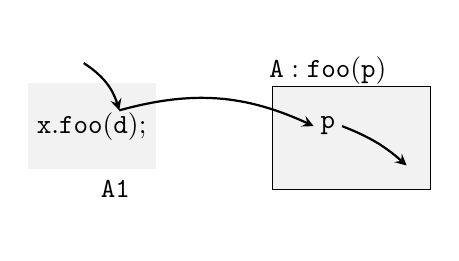
\begin{tikzpicture}
\def\base{1.5}
\def\x{3.0}
\def\xfd{0}
\draw [fill=black!5] (\base + \x + 1.3,0.5) rectangle (\base + \x - 0.7,-.8);
\node[minimum size=11mm] (cs) at (\base + \x, 0.7) {$\mathtt{A:foo(p)}$};
\node[minimum size=11mm, fill=black!5] (cs) at (\base + 0, 0 + \xfd) {$\mathtt{x.foo(d);}$};
\node[minimum size=11mm] (A) at (\base + 0.3, \xfd -.8) {$\mathtt{A1}$};
\node[minimum size=11mm] (p) at (\base + \x, 0) {$\mathtt{p}$};

% edges
\path[-stealth] (\base - 0.1, .8) edge [sloped, thick, bend left=20] (\base + 0.35, 0.2 + \xfd); % ... to d
\path[-stealth] (\base + 0.35, 0.2 + \xfd) edge [sloped, thick, bend left=20] (\base + \x - 0.18, 0.0); % d to p
\path[-stealth] (\base + \x + 0.18, 0.0) edge [sloped, thick, bend left=10] (\base + \x + 1, -
0.5); % p to ...
\end{tikzpicture}
}
        \vspace{-2ex}
        % \caption{Traditional CFL with pre-build call graph}
        \caption{Parameter passing without dispatch}
        \label{fig:approach0}
    \end{subfigure}
        \hspace{-2ex}
    \begin{subfigure}{.32\linewidth}
    \centering
    \resizebox{0.7\width}{0.7\height}{
        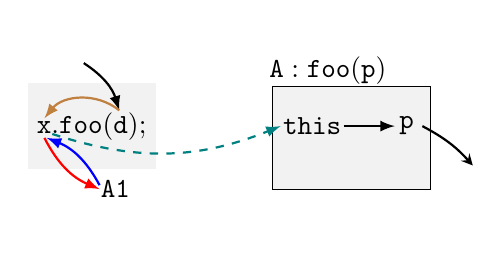
\begin{tikzpicture}
\def\base{1.5}
\def\x{3.0}
\def\xfd{0}
\draw [fill=black!5] (\base + \x + 1.3,.5) rectangle (\base + \x - 0.7,-.8);
\node[minimum size=11mm] (cs) at (\base + \x, .7) {$\mathtt{A:foo(p)}$};
\node[minimum size=11mm, fill=black!5] (cs) at (\base + 0, 0 + \xfd) {$\mathtt{x.foo(d);}$};
\node[minimum size=11mm] (A) at (\base + 0.3, \xfd - .8) {$\mathtt{A1}$};
\node[minimum size=11mm] (this) at (\base + \x - 0.2, 0) {$\mathtt{this}$};
\node[minimum size=11mm] (p) at (\base + \x + 1, 0) {$\mathtt{p}$};

% edges
\path[->] (\base -0.6, -0.15 + \xfd) edge [\colorb, thick, sloped, bend right=20] (\base + 0.1, -.8 + \xfd); % x to A
\path[->] (\base + 0.10, -0.75 + \xfd) edge [\colorc, sloped, thick, bend right=20] (\base -0.57, -0.15 + \xfd); % A to x

%\path[->] (0.1, -2.8) edge [sloped] (3.8, -0.2); % A to p
\path[->] (\base - 0.1, .8) edge [sloped, thick, bend left=20] (\base + 0.35, 0.2 + \xfd); % ... to d
\path[->] (\base + 0.35, 0.2 + \xfd) edge [\colora,sloped, thick, bend right=45] (\base -0.6, 0.1 + \xfd); % d to x 
\path[->] (\base -0.5, -0.1 + \xfd) edge [\colord, dashed, sloped, thick, bend right=20] (\base + \x - 0.6, 0.0); % x to this 
\path[->] (\base + \x + 0.2, 0) edge [sloped, thick] (\base + \x + 0.85, 0.0); % this to p 
\path[-stealth] (\base + \x + 1.2, 0.0) edge [sloped, thick, bend left=10] (\base + \x + 1.84, -
0.5); % p to ...
\end{tikzpicture}
}
        % \caption{New CFL with build-in call graph building}
        \vspace{-2ex}
        \caption{Dispatch at callsite}
        \label{fig:approach1}
    \end{subfigure}
    \hspace{-2ex}
    \begin{subfigure}{.32\linewidth}
    \centering
    \resizebox{0.7\width}{0.7\height}{
        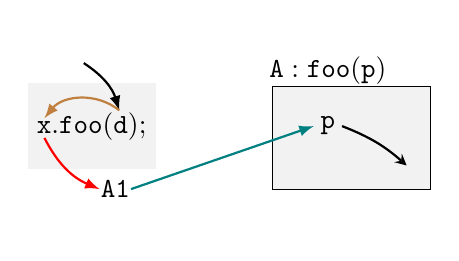
\begin{tikzpicture}
\def\base{1.5}
\def\x{3.0}
\def\xfd{0}
\draw [fill=black!5] (\base + \x + 1.3,.5) rectangle (\base + \x - 0.7,-.8);
\node[minimum size=11mm] (cs) at (\base + \x, .7) {$\mathtt{A:foo(p)}$};
\node[minimum size=11mm, fill=black!5] (cs) at (\base + 0, 0 + \xfd) {$\mathtt{x.foo(d);}$};
\node[minimum size=11mm] (A) at (\base + 0.3, \xfd -.8) {$\mathtt{A1}$};
\node[minimum size=11mm] (p) at (\base + \x, 0) {$\mathtt{p}$};

% edges
\path[->] (\base -0.6, -0.15 + \xfd) edge [\colorb, thick, sloped, bend right=20] (\base + 0.1, -.8 + \xfd); % x to A
\path[->] (\base + 0.5, -.8 + \xfd) edge [\colord, sloped, thick] (\base + \x - 0.18, 0.0); % A to p
\path[-stealth] (\base + \x + 0.18, 0.0) edge [sloped, thick, bend left=10] (\base + \x + 1, -
0.5); % p to ...
\path[->] (\base-0.1, .8) edge [sloped, thick, bend left=20] (\base + 0.35, 0.2 + \xfd); % ... to d
\path[->] (\base + 0.35, 0.2 + \xfd) edge [\colora,sloped, thick, bend right=45] (\base -0.6, 0.1 + \xfd); % d to x 
\end{tikzpicture}
}
        % \caption{CFL with build-in call graph building (dispatch on receiver object)}
        \vspace{-2ex}
        \caption{Dispatch at allocation site}
        \label{fig:approach2}
    \end{subfigure}
%   \vspace{-1.5ex}
    \caption{Three approaches for performing dynamic dispatch at a virtual callsite
    during parameter passing.}
    \label{fig:approach}
 %     \vspace{-2ex}
\end{figure*}

Below we discuss three possible dynamic dispatch approaches, illustrated in \Cref{fig:approach},  for handling parameter passing and explain why \LF is
designed to adopt a callsite-based approach (\Cref{fig:approach1}). 

As discussed in ~\Cref{subsubsec:manuLFC},  \manuLFC~\cite{sridharan2006refinement} solves
\kcs{k} by using a separate algorithm for call graph
construction (\Cref{fig:approach0}) and may thus cause \kcs{k} to lose precision 
(either directly (Sec.~\ref{sec:manuLFC+pre} and Sec.~\ref{sec:LFC+fly}) or  resorting to
a pre-analysis \cite{lu2021selective} (discussed in Sec.~\ref{sec:manuLFC+sep} and evaluated in \Cref{sec:evaluation})).

%The algorithm-assisted dispatching approach \cite{sridharan2005demand, sridharan2006refinement} in such case initiates and on-demand points-to analysis for the receiver variable and once its points-to information is obtained, the dispatching could be proceeded smoothly. 


In  \LF, passing an argument \texttt{d} at \texttt{x.foo(d)}  to a parameter will trigger
immediately a $\iflowsto$ traversal  looking for a
receiver object  of \texttt{x}, as symbolized by a red arrow (\textcolor{\colorb}{$\rightarrow$}) in \Cref{fig:approach1} (for performing dynamic dispatch at this callsite) and \Cref{fig:approach2} (for performing dynamic dispatch at the allocation site of the receiver object). 
\LF adopts the former approach
%(as described in Sec.~\ref{paragraph:chl1} and Sec.~\ref{paragraph:chl2} ) 
since the latter is infeasible.

Let us explain why the allocation-site-based dispatch (\Cref{fig:approach2}) is infeasible.
To handle parameter passing only (without considering method returns here), we need to extend \manuLF to become:
\begin{equation} 
% \footnotesize
\label{eqn:newFlows}
\begin{tabular}{rcl} 
$\flows$ & $\longrightarrow$ & $\cdots \mid \store[\texttt{m:i}]\ \iflowsto\ \load[\texttt{m:i}]$\\
$\iflows$ & $\longrightarrow$ &  $\cdots \mid  \iloadfield{\texttt{m:i}} \ \iflowsto \ \istorefield{\texttt{m:i}}$
\end{tabular}
\end{equation}
where  $\store[\texttt{m:i}]$ ($\load[\texttt{m:i}]$) is used to replace
 $\store[\texttt{i}]$ ($\load[\texttt{i}]$) in \Cref{fig:newcflpag}  in order
 to encode also the  signature of a method invoked at 
 $\mathtt{r}.\mathtt{m}(a_1, \dots, a_n)$. Thus, the \manuLFC-path in \Cref{eq:LFCPathCGPreciseI}
becomes:
%{
% \addtolength\abovedisplayskip{-.5ex}
% \addtolength\belowdisplayskip{-1.5ex}
\begin{equation} 
\footnotesize
  \centering
\label{eq:alterLFPath}
\begin{tabular}{l} 
\commentfont{O1}$\xrightarrow{\new}
\texttt{o1}\xrightarrow[\hat{\mathtt{c1}}]{\assign}
\texttt{o} \xrightarrow{\store[\texttt{f}]} \texttt{d}
\xrightarrow{\inew}$ 
\commentfont{D1} 
$ \xrightarrow{\new} \texttt{d}$ $\xrightarrow{\store[\texttt{foo:1}]}\texttt{x}\xrightarrow[\check{\mathtt{c1}}]{\iassign}\texttt{a}
\xrightarrow{\inew}$\commentfont{A1}$\xrightarrow{\load[\texttt{foo:1}]}\texttt{p}
    \xrightarrow{\load[\texttt{f}]} \texttt{v}
$
% \\[3ex]
% \begin{tikzpicture}[-, remember picture,overlay]
% \def\lx{6.2}\def\ly{.99}
% \def\dy{.54}\def\ny{.07}
% \draw(\lx, \ly) -- (\lx+.1, \ly) -- (\lx+.1, \dy);
% \draw[dashed] (\lx+.1, \dy) -- (-.12,\dy);
% \draw(-.12,\dy) -- (-.12, \ny);
% \draw[->] (-.12, \ny) -- (0.06, \ny);
% \end{tikzpicture}
% \footnotesize
\end{tabular}
\end{equation}
%}
where we have
$\texttt{d}\xrightarrow{\store[\texttt{foo:1}]}\texttt{x}$
(\textcolor{\colora}{$\rightarrow$}), 
$\texttt{x} \xrightarrow[\check{\mathtt{c1}}]{\iassign}\texttt{a} \xrightarrow{\inew}$\commentfont{A1}
(\textcolor{\colorb}{$\rightarrow$}), and
\commentfont{A1}$\xrightarrow{\load[\texttt{foo:1}]}\texttt{p}$
(\textcolor{\colord}{$\rightarrow$}). However, 
 \commentfont{O1} flows to \texttt{v} under \emptyctx incorrectly (with
$\hat{\texttt{c1}}$ and $\check{\texttt{c1}}$ being matched). \hl{Due to the
nature of object-sensitivity (where receiver objects are used as context elements)},
 the CFL-reachability formulation for object-sensitive pointer analysis \cite{lu2019precision, lu2021eagle} (as reviewed briefly in \Cref{sec:relatedwork:cfl}) works well with the allocation-site-based dispatch approach.



% There seems to be another choice here. 
% In the above process, when we find the receiver object, we have gathered all the information needed for dispatching. One would ask why we must go back to the callsite. It is true if only context-insensitive analysis is considered. For example, we can use \argrec to mark the beginning of searching for a receiver object. After we find the specific object, we need to know which callsite (to be precise, its method signature) is being processed to dispatch correct method according to the type and method signature. We also need to know which parameter is being passed in order to pass the correct parameter after dispatch. This can be solved by adding a set of balanced parentheses with method signature and parameter: When we start looking for receiver object at \argrec, we introduce the method signature of the callsite and the target parameter on the stack. That is, \argrec[m:i]. After finding the specific object, we can match it with, say, \recparm[m:i] to pass the argument to the correct formal parameter, which can be established statically. That is, the previous "entry" edge in \rulename{P-Call} is parsed with \argrec[m:i] \iflowsto \recparm[m:i] rather than a simple \assign edge as before. And the non-terminal \flows in \cref{eqn:callsiteLF} is changed to:

% "exit" edge in \rulename{P-Call} and \iflows in \cref{eqn:callsiteLF} should be changed accordingly but omitted here. The process of this kind of way of handling of parameter passing is illustrated in \cref{fig:approach1}.


%However, the context after the parameter passing is different from the traditional formulation \cite{sridharan2005demand, sridharan2006refinement}. Consider the following flow path from 
%\commentfont{O1} to \texttt{v} in \Cref{fig:motivatingExample} (again but this time expressed by $\mathcal{L}_{F'C}$ as \Cref{eq:alterLFPath}):

% For example, if we simply apply \cref{eqn:newFlows}, we will find that although we can find the correct formal parameter for this single parameter passing, the context for \texttt{p} or \texttt{v} after the parameter passing is not as expected. We note the language $L_F$ modified with \cref{sec:newFlows} as $L_{F'}$. The path from \commentfont{O1} to 
% \texttt{v} is expressed by $L_{FC}$ as \cref{eq:LFCPathCGPreciseI} but is expressed by $L_{F'C}$ as \cref{eq:alterLFPath}:
\begin{comment}
The $L_C(p_{\color{purple}{\mathtt{O1}},\texttt{v}})=\hat{\mathtt{c1}}\hat{\mathtt{c3}}$ in \Cref{eq:LFCPathCGPreciseI} but \LC$(p_{\color{purple}{\mathtt{O1}},\texttt{v}})=\hat{\mathtt{c1}}\check{\mathtt{c1}}$ in \Cref{eq:alterLFPath}, resulting in 
inconsistent calling contexts for \texttt{v} (i.e., $[\mathtt{c3}, \mathtt{c1}]$ and \emptyctx ~ respectively) when the parameter passing is completed.
\end{comment}
%We know that the callsite-sensitivity is modeling call stacks, so $\mathcal{L}_{F'C}$ is incorrect
%for a callsite-sensitive analysis. 
%Note that attempting to encode context information into below-edges in \pag (e.g., replacing $\xrightarrow{\load[\texttt{foo:1}]}$ in \Cref{eq:alterLFPath} with $\xrightarrow[\hat{\texttt{c1}};\hat{\texttt{c3}}]{\load[\texttt{foo:1}]}$) is also infeasible as one method may be invoked under different calling contexts with a same receiver object and statically establishes \LC strings from receiver variables to receiver objects would be another challenge. 

%By returning to the callsite after finding the receiver object, changing the dispatching location to callsite, and together with the following \LR, \challenge{3} can be addressed.


\subsubsection{The $L_R$ Language}
\label{subsubsec:newLR}

%Given \LF (defined in \Cref{eqn:finalNewLF}) and $\LC=\manuLC$ (defined in \Cref{eqn:callsiteLC}), we have obtained a new language: \capLFC. However,
%\LFC solves \kcs{k} soundly but less precisely than \manuLFCDD (Lemma~\ref{thm:lfc-imprecise}).

\LFC is sound but imprecise. We  use two examples given in
\Cref{fig:LFC-imprecision-callsite} and \Cref{fig:LFC-imprecision-context} to illustrate the imprecision of \LFC and highlight the two roles that \LR plays
in \LFCR. 

\LFC can lose precision caused by an incorrect  dispatch callsite. Consider the following two \LFC-paths in the PAG of \Cref{fig:LFC-imprecision-callsite} (by ignoring  the boxed labels $\hat{\boxed{\texttt{c1}}}$, $\check{\boxed{\texttt{c1}}}$ and $\check{\boxed{\texttt{c2}}}$ for now):
\begin{equation} 
\label{eq:ex2-inv-c1-site}
  \centering
\begin{tabular}{l} 
\commentfont{O1}$\xrightarrow{\new[\texttt{O}]} \texttt{o1} 
\xrightarrow[\hat{\boxed{\texttt{c1}}}]{\store[1]} \texttt{a} 
\xrightarrow{\inewfield{\texttt{A}}}
$
\commentfont{A1}
$ \xrightarrow{\new[\texttt{A}]} \texttt{a}$
$\xrightarrow[\check{\boxed{\texttt{c1}}}]{\assign} \texttt{a\#c1}
\xrightarrow[\hat{\texttt{c1}}]{\indispatch[\texttt{A}]} \texttt{this}^{\texttt{m}} 
\xrightarrow{\load[1]} \texttt{p}
$
\end{tabular}
\end{equation}

%\bigskip
\vspace*{-1ex}

\begin{equation} 
\label{eq:ex2-inv-c2-site}
  \centering
\begin{tabular}{l} 
\commentfont{O1}$\xrightarrow{\new[\texttt{O}]} \texttt{o1} 
\xrightarrow[\hat{\boxed{\texttt{c1}}}]{\store[1]} \texttt{a} 
\xrightarrow{\inewfield{\texttt{A}}}
$
\commentfont{A1}
$ \xrightarrow{\new[\texttt{A}]} \texttt{a}$
$\xrightarrow[\check{\boxed{\texttt{c2}}}]{\assign} \texttt{a\#c2}
\xrightarrow[\hat{\texttt{c2}}]{\indispatch[\texttt{A}]} \texttt{this}^{\texttt{n}} 
\xrightarrow{\load[1]} \texttt{q}
$
\end{tabular}
\end{equation}

These two \LFC-paths both keep track of where \commentfont{O1}  flows to in the
\pag of this program.
According to the first \LFC-path, \commentfont{O1} flows to \texttt{p} as 
expected. However, due to the existence of the second \LFC-path, 
\commentfont{O1} can also flow to \texttt{q} spuriously as the $\iflowsto$ traversal for finding the receiver object of \texttt{a} is triggered at callsite \texttt{c1} but the dispatch ends up happening at  callsite \texttt{c2}. To eliminate such precision loss, \LR requires  boxed edge labels to be matched as balanced parentheses. As a result,  the first \LFC-path in \Cref{eq:ex2-inv-c1-site} will be considered
as a valid \LFCR-path (since $\hat{\boxed{c1}}$ is matched by $\check{\boxed{c1}}$) but  the second \LFC-path in \Cref{eq:ex2-inv-c2-site} will be ruled out (since $\hat{\boxed{c1}}$ is not matched by $\check{\boxed{c2}}$). 

\LFC can also lose precision caused by an incorrect dispatch context.  
Consider the following two \LFC-paths in the PAG of \Cref{fig:LFC-imprecision-context}
(by ignoring  the boxed labels $\hat{\boxed{\texttt{c3}}}$ and $\check{\boxed{\texttt{c3}}}$ 
for now):


\begin{figure}
\begin{mdframed}[
align=center,
usetwoside=false,
 rightmargin=3cm,
innerleftmargin=1.0ex,
innerrightmargin=-20.0ex
innertopmargin=0.2ex,
innerbottommargin=0.2ex
]

\begin{minipage}{0.4\linewidth}
\begin{lstlisting}[language=java, basicstyle=\linespread{0.8}]
static void main() {
  A a = new A(); // A1
  O o1 = new O(); // O1
  O o2 = new O(); // O2
  a.m(o1); // c1
\end{lstlisting}
\end{minipage}
\hspace{-2ex}
\begin{minipage}{0.4\linewidth}
\begin{lstlisting}[language=java, firstnumber=6, basicstyle=\linespread{0.8}]
  a.n(o2); } // c2
class O { }
class A {
  void m(Object p) { ... }
  void n(Object q) { ... } }
\end{lstlisting}
\end{minipage}

\end{mdframed}
\caption{An example for illustrating the imprecision of \LFC caused by an
incorrect dispatch site.
    \label{fig:LFC-imprecision-callsite}}
\end{figure}



\begin{figure}
\begin{mdframed}[
align=center,
usetwoside=false,
rightmargin=3cm,
innerleftmargin=1.0ex,
innerrightmargin=-20.0ex
innertopmargin=0.2ex,
innerbottommargin=0.2ex
]

\begin{minipage}{0.4\linewidth}
\begin{lstlisting}[language=java, basicstyle=\linespread{0.8}]
class A {
  O id(O p) { return p; } }
class O { }
static O wid(A a, O o) {
  O v = a.id(o); // c3
  return v;
}
\end{lstlisting}
\end{minipage}
\hspace{-2ex}
\begin{minipage}{0.4\linewidth}
\begin{lstlisting}[language=java, firstnumber=8, basicstyle=\linespread{0.8}]
static void main() {
  A a1 = new A(); // A1
  O o1 = new O(); // O1
  O o2 = new O(); // O2
  O v1 = wid(a1, o1); // c1
  O v2 = wid(a1, o2); // c2
}
\end{lstlisting}
\end{minipage}
\end{mdframed}
\caption{An example for illustrating the imprecision of \LFC caused by an
incorrect dispatch context.
    \label{fig:LFC-imprecision-context}}
\end{figure}

\begin{equation} 
% \scriptsize
\label{eq:ex2-inv-c1}
  \centering
\begin{tabular}{l} 
\commentfont{O1}$\xrightarrow{\new[\texttt{O}]} \texttt{o1}
\xrightarrow[\hat{\texttt{c1}}]{\assign} \texttt{o} 
\xrightarrow[\hat{\boxed{\texttt{c3}}}]{\store[1]} \texttt{a} 
\xrightarrow[\check{\texttt{c1}}]{\iassign} \texttt{a1}
\xrightarrow{\inewfield{\texttt{A}}}
$
\commentfont{A1}
$ \xrightarrow{\new[\texttt{A}]} \texttt{a1} 
\xrightarrow[\hat{\texttt{c1}}]{\assign} \texttt{a}$ \\[5ex]
\begin{tikzpicture}[-, remember picture,overlay]
\def\lx{10.4}\def\ly{1.4}
\def\dy{.76}\def\ny{.065}
\draw(\lx, \ly) -- (\lx+.1, \ly) -- (\lx+.1, \dy);
\draw[dashed] (\lx+.1, \dy) -- (-.12,\dy);
\draw(-.12,\dy) -- (-.12, \ny);
\draw[->] (-.12, \ny) -- (0.06, \ny);
\end{tikzpicture}
$\xrightarrow[\check{\boxed{\texttt{c3}}}]{\assign} \texttt{a\#c3}
\xrightarrow[\hat{\texttt{c3}}]{\indispatch[\texttt{A}]} \texttt{this}^{\texttt{id}} 
\xrightarrow{\load[1]} \texttt{p} \xrightarrow{\store[\ret]} \texttt{this}^{\texttt{id}} 
\xrightarrow[\check{\texttt{c3}}]{\iindispatchfield{\texttt{A}}} \texttt{a\#c3}
$ \\[5ex]
\begin{tikzpicture}[-, remember picture,overlay]
\def\lx{10.4}\def\ly{1.4}
\def\dy{.76}\def\ny{.065}
\draw(\lx, \ly) -- (\lx+.1, \ly) -- (\lx+.1, \dy);
\draw[dashed] (\lx+.1, \dy) -- (-.1,\dy);
\draw(-.12,\dy) -- (-.12, \ny);
\draw[->] (-.12, \ny) -- (0.06, \ny);
\end{tikzpicture}
$\xrightarrow[\hat{\boxed{\texttt{c3}}}]{\iassign} \texttt{a}
\xrightarrow[\check{\texttt{c1}}]{\iassign} \texttt{a1} 
\xrightarrow{\inewfield{\texttt{A}}}$
\commentfont{A1}$\xrightarrow{\new[\texttt{A}]} \texttt{a1}
\xrightarrow[\hat{\texttt{c1}}]{\assign} \texttt{a}
\xrightarrow[\check{\boxed{\texttt{c3}}}]{\load[\ret]}
\texttt{v} \xrightarrow[\check{\texttt{c1}}]{\assign} 
\texttt{v1}
$
\end{tabular}
\end{equation}

\bigskip

\begin{equation} 
% \scriptsize
\label{eq:ex2-inv-c2}
  \centering
\begin{tabular}{l} 
\commentfont{O1}$\xrightarrow{\new[\texttt{O}]} \texttt{o1}
\xrightarrow[\hat{\texttt{c1}}]{\assign} \texttt{o} 
\xrightarrow[\hat{\boxed{\texttt{c3}}}]{\store[1]} \texttt{a} 
\xrightarrow[\check{\texttt{c1}}]{\iassign} \texttt{a1}
\xrightarrow{\inewfield{\texttt{A}}}
$
\commentfont{A1}
$ \xrightarrow{\new[\texttt{A}]} \texttt{a1} 
\xrightarrow[\hat{\texttt{c2}}]{\assign} \texttt{a}$ \\[5ex]
\begin{tikzpicture}[-, remember picture,overlay]
\def\lx{10.4}\def\ly{1.4}
\def\dy{.76}\def\ny{.065}
\draw(\lx, \ly) -- (\lx+.1, \ly) -- (\lx+.1, \dy);
\draw[dashed] (\lx+.1, \dy) -- (-.12,\dy);
\draw(-.12,\dy) -- (-.12, \ny);
\draw[->] (-.12, \ny) -- (0.06, \ny);
\end{tikzpicture}
$\xrightarrow[\check{\boxed{\texttt{c3}}}]{\assign} \texttt{a\#c3}
\xrightarrow[\hat{\texttt{c3}}]{\indispatch[\texttt{A}]} \texttt{this}^{\texttt{id}} 
\xrightarrow{\load[1]} \texttt{p} \xrightarrow{\store[\ret]} \texttt{this}^{\texttt{id}} 
\xrightarrow[\check{\texttt{c3}}]{\iindispatchfield{\texttt{A}}} \texttt{a\#c3}
$ \\[5ex]
\begin{tikzpicture}[-, remember picture,overlay]
\def\lx{10.4}\def\ly{1.4}
\def\dy{.76}\def\ny{.065}
\draw(\lx, \ly) -- (\lx+.1, \ly) -- (\lx+.1, \dy);
\draw[dashed] (\lx+.1, \dy) -- (-.1,\dy);
\draw(-.12,\dy) -- (-.12, \ny);
\draw[->] (-.12, \ny) -- (0.06, \ny);
\end{tikzpicture}
$\xrightarrow[\hat{\boxed{\texttt{c3}}}]{\iassign} \texttt{a}
\xrightarrow[\check{\texttt{c2}}]{\iassign} \texttt{a1} 
\xrightarrow{\inewfield{\texttt{A}}}$
\commentfont{A1}$\xrightarrow{\new[\texttt{A}]} \texttt{a1}
\xrightarrow[\hat{\texttt{c2}}]{\assign} \texttt{a}
\xrightarrow[\check{\boxed{\texttt{c3}}}]{\load[\ret]}
\texttt{v} \xrightarrow[\check{\texttt{c2}}]{\assign} 
\texttt{v2}
$
\end{tabular}
\end{equation}

These two \LFC-paths differ only in their underlying contexts  and  target variables used:
the second  can be obtained from the first by
replacing each occurrence of \texttt{c1} with \texttt{c2} and \texttt{v1} with \texttt{v2}.
Both \LFC-paths  keep track of where \commentfont{O1} will flow to,
starting from the call ``\inline{wid(a1,o1); // c1}''. According to the first
\LFC-path,  \texttt{v1} points to \commentfont{O1} as
expected. However, due to the existence of the second \LFC-path, 
\commentfont{O1}, which comes from callsite \texttt{c1}, will flow into \texttt{v2} at callsite \texttt{c2} spuriously.
Consider the dynamic dispatch that happens at ``\inline{a.id(o); // c3}''
due to the call\linebreak  ``\inline{wid(a1,o1); // c1}''. 
In the first \LDC-path,
\texttt{a} starts with pointing to \commentfont{A1} under
 [\texttt{c1}]
 during its $\iflowsto$  traversal (to find what \texttt{a} points to)
 and ends up with pointing  to \commentfont{A1} under  
  [\texttt{c1}] during
 the ensuing
 $\flowsto$ traversal.
 This $\flowsto$ traversal can
 happen from the call  ``\inline{wid(a1,o1); // c1}''. However, in the second \LDC-path,
\texttt{a} starts also with pointing to \commentfont{A1} under
 [\texttt{c1}]
 during its $\iflowsto$  traversal but ends up with pointing  to \commentfont{A1} under  
  [\texttt{c2}] during
 the ensuing
 $\flowsto$ traversal. This  $\flowsto$ traversal cannot
 happen from the call  ``\inline{wid(a1,o1); // c1}''.

\begin{comment}
In both \LFC-paths,  the same $\iflowsto$  traversal is performed to find that
\texttt{a}  points to \commentfont{A1} under $\CC=[\texttt{c1}]$. However,
when returning to \texttt{a} during the following
 $\flowsto$ traversal, we traverse the same $\iflowsto$-path backwards
 under also $[\texttt{c1}$] (which can happen under under $\CC=[\texttt{c1}$]
 in the first \LFC-path but 
 and
 ends up with pointing  to \commentfont{A1} under also 
  [\texttt{c1}] during
  (which is possible under $\CC=[\texttt{c1}$]. 
 


This path contains two dispatch paths for ``\inline{a.id(o) // c3}'', 
one for  passing \texttt{o} to \texttt{p} and one for returning 
 \texttt{p} back to the same callsite. 
The first one is invalid, since \texttt{a} starts with pointing to \commentfont{A1} under
 [\texttt{c1}]
 during its $\iflowsto$  traversal but ends up with pointing  to \commentfont{A1} under  
  [\texttt{c2}] during
 the ensuing
 $\flowsto$ traversal, violating \dispatchconTwo. Thus, \LFC enables
 \commentfont{O1} passed at callsite \texttt{c1} to flow into \texttt{v2}
 at callsite \texttt{c2}  spuriously.
\end{comment}

Consider a virtual callsite 
``$\mathtt{r}.\mathtt{m}(a_1, \dots, a_n); ~ // \mathtt{c}$'' with a reference to
\Cref{eq:proof-valid-DP}.
In general, when performing a $\iflowsto$ traversal to find that 
$\mathtt{r}$ points to a receiver object $O$ under $[\check{c_1},...,\check{c_k}]$,
\LR must be designed to ensure that we can return from $O$ to $\mathtt{r}$  by performing a $\flowsto$ traversal
under exactly $[\hat{c_k},...,\hat{c_1}]$ in order to avoid passing arguments spuriously.

To address \challenge{3} (i.e., the two sources of imprecision above), we  introduce  a third CFL \LR: 
\begin{equation}
\footnotesize
    \label{eqn:callsiteLR}
    \begin{tabular}{rcl}
$\recoveredctx$ & $\longrightarrow$ & $\recoveredctx~\hat{c} \mid \recoveredctx~\check{c} \mid \recoveredctx~ \siterecovered \mid \epsilon$\\[1ex]
$\siterecovered$ & $\longrightarrow$ & $\hat{\boxed{c}} ~ \ctxrecovered ~ \check{\boxed{c}}$\\[1ex]
$\ctxrecovered$ & $\longrightarrow$ & $\matched ~ \ctxrecovered \mid \ctxrecovered ~ \matched \mid\check{c} ~ \ctxrecovered ~ \hat{c} \mid \epsilon$\\[1ex]
$\matched$ & $\longrightarrow$ & $\matched ~ \matched \mid \hat{c} ~ \matched ~ \check{c} \mid \siterecovered\mid\epsilon$ \\[1ex]
    \end{tabular}
\end{equation}
%where its terminals are the below-edge labels, $\hat{c}$ and$\check{c}$, $\hat{\boxed{c}}$, and $\check{\boxed{c}}$, in the \pag. 

All the above-edge labels are handled similarly as in the case of \manuLC. By
decomposing each double-label edge into a sequence of
two single-label edges as described in
\Cref{subsubsec:CFLReachability}, $\matched$ is extended by adding
a new production 
$\matched \longrightarrow  \reg{above-edge-label}$, where
 the new non-terminal
\reg{above-edge-label}  is defined in terms of all the original above-edge
labels  in a given \pag.


With \LR being incorporated into
\LFC, the resulting language \capLFCR will be precise in handing parameter passing for virtual callsites. Let us return  to  the two paths given in \Cref{eq:ex2-inv-c1} and
\Cref{eq:ex2-inv-c2} with  $\hat{\boxed{\texttt{c3}}}$
and $\check{\boxed{\texttt{c3}}}$) being considered.
The first one is an \LFCR-path but the second is not. 
The first one is an  \LFCR-path, since we start the dynamic dispatch process
at callsite \texttt{c3} (marked by the first 
  $\hat{\boxed{\texttt{c3}}}$)
under context $[\texttt{c1}]$ and return to the same callsite under
the same context at the end of this dynamic dispatch process (marked by the first
  $\check{\boxed{\texttt{c3}}}$) even though \texttt{c1} is lost, i.e.,
  balanced out due to 
  $\hat{{\texttt{c1}}}\check{{\texttt{c1}}}$ just after the first
  $\mathtt{a}\xrightarrow[\check{{\mathtt{c1}}}]{\iassign} \mathtt{a1}$ edge is
  traversed.
  The second one is \emph{not} an  \LFCR-path, since even though we also start the dynamic dispatch process
at callsite \texttt{c3} (marked by the first 
  $\hat{\boxed{\texttt{c3}}}$)
under context $[\texttt{c1}]$, we end up returning to the same callsite under
a different and thus incorrect context, $[ \texttt{c2}]$, at the end of this dynamic dispatch process (marked by the first
  $\check{\boxed{\texttt{c3}}}$).
  %once \texttt{c1} is    balanced out due to   $\hat{{\texttt{c1}}}\check{{\texttt{c1}}}$ just after the first  $\mathtt{a}\xrightarrow[\check{{\mathtt{c1}}}]{\iassign} \mathtt{a1}$ edge is  traversed.
As a result, \LFCR will conclude that
\commentfont{O1} is pointed to by \texttt{v1} but not by \texttt{v2} as desired.

Below, we give a formal development of \LR  and then
prove the precision of \LFCR.

We can obtain the points-to set of a variable $v$,  $\pointsto(v, c_v)$,
from \LFC as follows. 
Given an \LC-path $p$ with its label being
$\LC(p)=\ell_1,\dots,\ell_n$, where each $\ell_i$ is an entry or exit
context label in an inter-procedural \assign edge,
%(implying that  $\LC(p)\in\LC$),  
 the inverse of $p$, i.e.,
$\overline{p}$ has the label
$\LC(\overline{p})=\overline{\ell_n},\dots,
\overline{\ell_1}$.
% (implying that  $\LC(\overline{p})\in\LC$). 
By splitting $p$ into a sub-path $p^\exit$ followed
by a sub-path $p^\entry$, we can define $\LC^\exit(p)=\LC(p^\exit)$ 
and $\LC^\entry(p)=\LC(p^\entry)$, where
$\LC(p) = \LC^\exit(p)\LC^\entry(p)$, such that  $\LC^\exit(p)$ ($\LC^\entry(p)$) is
derived from 
\gramexit (\gramentry) in \LC's grammar (\Cref{eqn:callsiteLC}).
Let $s\in \LC$.
Let $\BalParen{s}$ return the canonical form of $s$ with
all its balanced contexts (i.e., parentheses) removed.
If $c$ is a string of exit contexts  of the form
$\check{c_1}
\dots\check{c_n}$, we write 
$\RawCtxCheck{c} = [c_1,\dots,c_n]$ to turn it into a context representation
(by noting that $\RawCtxCheck{\epsilon}=\emptyctx$).



\begin{comment}
Our CFL-reachability formulation
of \kcs{k}, defined by 
\capLFCR, discovers the points-to information in \pag as follows.
A path $p$ from $O$ to $v$ in \pag can be identified as a context-sensitive \flowsto relation iff $p$ is both (1) a $\flowsto$ path in \LF, where  $O\;\flowsto\; v$, (2) a realizable path in \LC, where 
$\realizable \Longrightarrow^* \mathcal{L}_C(p)$, and (3) a $W$ path in \LR, where $W \Longrightarrow^* \mathcal{L}_R(p)$, yielding the following
context-sensitive points-to relation:
\end{comment}

Given an \LFC-path  $p$ starting from an object $O$ to a variable $v$, we can deduce the following points-to relation with the contexts of $O$ and $v$ being spelt out clearly:
%{
%\addtolength\abovedisplayskip{-.3ex}
%\addtolength\belowdisplayskip{-.3ex}
\begin{equation}
\label{eq:pt-ctx}
%\hspace*{-1ex}
\begin{tabular}{@{}r@{\ }c@{\ }l@{}}
$\langle O,\RawCtxCheck{\BalParen{\LC^\exit(p)}}\rangle$ & $\quad\in \quad$  &
$\pointsto(v, \RawCtxHat{\overline{\BalParen{\LC^\entry(p)}}}
)$\\
\end{tabular}
\end{equation}

\begin{comment}
where
\begin{eqnarray}
\label{eq:pt-ctx}
\begin{tabular}{@{}r@{\ }c@{\ }l@{}}
$ctx(\mathcal{L}_C^\entry(p))$ & $\eqdef$ & sequence of unbalanced  $\check{c}$\,'s in\\&& $\overline{\mathcal{L}_C^\entry(p)}$ with their hats elided;\\
$ctx(\mathcal{L}_C^\exit(p))$ & $\eqdef$ & sequence of  unbalanced  $\check{c}$\,'s in\\&&  
$\mathcal{L}_C^\exit(p)$ with their checks elided.
\end{tabular}
%\hspace*{-3ex}
\end{eqnarray}
\end{comment}
Let us consider an example.
Let $p_{{\color{purple}\texttt{O1}},\texttt{v}}$ be the \LFC-path in \Cref{eq:ex-patho1-to-v} (by 
ignoring
  $\hat{\boxed{\texttt{c3}}}$
and $\check{\boxed{\texttt{c3}}}$). By definition, 
$\LC(p_{{\color{purple} \texttt{O1}},\texttt{v}})=\hat{\texttt{c1}}\check{\texttt{c1}}\hat{\texttt{c1}}
\hat{\texttt{c3}}$, where
$p_{{\color{purple}\texttt{O1}},\texttt{v}}^\exit$ can be interpreted
as the sub-path from \commentfont{O1} to \commentfont{A1} and $p_{{\color{purple} \texttt{O1}},\texttt{v}}^\entry$
as the sub-path from \commentfont{A1} to \texttt{v}. Thus,
$\LC^\exit(p_{{\color{purple}\texttt{O1}},\texttt{v}})  =\hat{\texttt{c1}}\check{\texttt{c1}}$ and $\LC^\entry(p_{{\color{purple}\texttt{O1}},\texttt{v}})=\hat{\texttt{c1}}
\hat{\texttt{c3}}$. Since
$\RawCtxCheck{\BalParen{\hat{\texttt{c1}}\check{\texttt{c1}}}}
=\RawCtxCheck{\epsilon}=\emptyctx$ and
$\RawCtxHat{\overline{\BalParen{\hat{\texttt{c1}}\hat{\texttt{c3}}}}}
=
\RawCtxHat{\overline{{\hat{\texttt{c1}}\hat{\texttt{c3}}}}}
=
\RawCtxHat{{{\check{\texttt{c3}}\check{\texttt{c1}}}}}
=
[{{{{\texttt{c3}},{\texttt{c1}}}}}]
$, we have:
\begin{equation*}
 \langle {\color{purple}\texttt{O1}},\emptyctx \rangle\quad \in\quad
\pointsto(\texttt{v}, [\texttt{c3},\texttt{c1}])
\end{equation*}



\LFC can lose precision  since, for some \LFC-paths, its sub-paths responsible for
performing dynamic dispatch can be spurious. Consider a virtual callsite $ \texttt{r}.\mathtt{m}(a_1, \dots, a_n) ~ //~ c$.  
Before passing an argument $a_i$ into (or receiving a return value from) a
method invoked, \LFC performs dynamic dispatch  
by carrying out
the following alias-related traversal on its receiver variable $\mathtt{r}$:
\begin{equation}
% \footnotesize
\label{eq:dispatchpath}
\cdots \xrightarrow[\hat{\boxed{c}}]{\ell} \mathtt{r} ~
\iflowsto ~ O ~ \flowsto ~\mathtt{r}'
% ~ \alias\quad~ r'
 \xrightarrow[\check{\boxed{c'}}]{\assign} \mathtt{r}'\#c'
 \xrightarrow[\hat{c'}]{\indispatch[\texttt{\_}]}\cdots
 %\texttt{this}^\texttt{T:foo()}
 \end{equation}
 where $\ell$ is $\storefield{i}$ (in passing $a_i$) or $\iloadfield{0}$ (in
 retrieving a return value). Such a path, which starts from 
 $\hat{\boxed{c}}$ and ends at $\check{\boxed{c'}}$, is called 
 a \textit{dispatch path}, which
is \emph{valid} if  two conditions are met:
\begin{itemize}
    \item \dispatchconOne: $c=c'$ (implying that $\mathtt{r}=\mathtt{r}'$), and
%    \item \dispatchconTwo:  $\mathtt{r}$ and $\mathtt{r}'$ are aliased  under   the same context.
    \item \dispatchconTwo: $O$ is pointed by both $\mathtt{r}$ and $\mathtt{r}'$ (which
    are thus aliases) under   exactly the same context.
\end{itemize} 

 However, \LFC can only ensure that $\mathtt{r}$ and $\mathtt{r}'$ are aliases but with no guarantee for the validity of
 this dispatch path.
To filter out all  \LFC-paths containing invalid dispatch paths, we use  \LR 
given earlier
to enforce
\dispatchconOne and \dispatchconTwo, thereby addressing 
\challenge{3} by
restoring  the callsite and context of $\mathtt{r}$. In particular,
 the $\siterecovered$-production  enforces
\dispatchconOne, and the set of $\ctxrecovered$-productions, together with the set of $\matched$-productions, enforce \dispatchconTwo.
% by not only matching method calls and returns as a balanced-parentheses problem but also ensuring contexts to be restored when dispatching:
%\input{languageC.tex}
%{
%\addtolength\abovedisplayskip{-.5ex}
%\addtolength\belowdisplayskip{-.5ex}
% \begin{equation}
% \label{eqn:callsiteLC}
% \footnotesize
%     \begin{split}
% \textsf{realisable} \longrightarrow \textsf{exit} ~ \textsf{entry} \\
% \textsf{exit} \longrightarrow \textsf{exit} ~ \textsf{B} \mid \textsf{exit} \ \check{c} \mid \epsilon \\ 
% \textsf{entry} \longrightarrow \textsf{entry} ~ \textsf{B} \mid \textsf{entry} \ \hat{c} \mid \epsilon \\
% \textsf{B} \longrightarrow \textsf{B} ~ \textsf{B} \mid \hat{c} ~ \textsf{B} ~ \check{c} \mid \hat{\boxed{c}} ~ R ~ \check{\boxed{c}} \mid \epsilon \\
% R \longrightarrow B ~ R \mid R ~ B \mid \check{c} ~ R ~ \hat{c} \mid H\\
% H \longrightarrow B ~ H \mid H ~ B \mid \hat{c} ~ H ~ \check{c} \mid \epsilon\\
%     \end{split}
% \end{equation}

%, with both being mutually recursive due to the recursive nature of \kcs{k}.

%\LR is an supplementary language of \LC for supporting dynamic dispatching. 
%Below, we highlight that how we address \challenge{3} in \LR. 


%\Cref{thm:lfc-imprecise} has shown that \LFC is a superset of \manuLFC, we must show how the extra words are correctly filtered out by \LR.
%happens under  the same context as in the
%\manuLFC-based formulation (with dynamic dispatch done separately), by exploiting the balanced matching property of virtual call dispatching.
\begin{comment}
By construction, \LFC enforces that we find receiver object from the receiver variable of a callsite (say, $x$ on $c$) and return to the receiver variable of a callsite (say, $x'$ on $c'$). But it only ensures $x$ and $x'$ are alias. It guarantees neither $c$ and $c'$ are same nor $x$ and $x'$ are context-sensitively the same variable (under the same context). This can be respectively addressed in two cases: {\bf case 1.} By using a balanced parentheses matching of $\hat{\boxed{c}}$ and $\check{\boxed{c}}$, we guarantee $c$ and $c'$ are same. {\bf case 2.} The production rule for non-terminal $Y$ between $\hat{\boxed{c}}$ and $\check{\boxed{c}}$ enforces we start and end at the same receiver variable. Below, we discuss it in details.
\end{comment}
%As stated earlier in \LF, we require that $\store[\texttt{i}]$ matched by $\load[\texttt{i}]$ and type $\texttt{t}$ in $\indispatch[\texttt{t}]$
%must be consistent with the one in $\new[\texttt{t}]$ of current $\flowsto$ value flow. However, these could not guarantee that dispatching is correct as we have chosen to perform dispatching at callsites (\Cref{fig:approach2}).

\begin{comment}


\paragraph{Imprecision of \LFC}
\label{sec:LFC-impre}

We look at two  examples  to understand why \LFC fails to enforce
\dispatchconOne and \dispatchconTwo. 

Consider the following simple code snippet:
%where \texttt{A} is modified by adding a new method definition ``\lstinline[language=java]!void goo(D s){}!''):
\vspace{.5ex}
\begin{mdframed}[
%innermargin =-2ex,
%  rightmargin=-1cm,
innerleftmargin=-0.3ex,
innerrightmargin=-1.0ex,
innertopmargin=0.0ex,
innerbottommargin=0.2ex
]
\begin{lrbox}{\mybox}
\begin{lstlisting}[language=java, basicstyle=\linespread{0.8}\small, numbers=none]
D d1 = new D(); // D1
D d2 = new D(); // D2
A a = new A(); // A1
a.foo(d1); // c1
a.foo(d2); // c2
\end{lstlisting}
\end{lrbox}
\scalebox{0.9}{\usebox{\mybox}}
\end{mdframed}
where classes \texttt{A} and \texttt{D} are from \Cref{fig:motivatingExample}.
The following path is accepted by \LFC (as an \LFC-path) but rejected by \LFCR:
\begin{equation} 
% \scriptsize
  \centering
\label{eq:CH3Case2}
\begin{tabular}{@{\hspace{-2ex}}l} 
\commentfont{D1}$\xrightarrow{\!\!\new[\texttt{D}]\!\!}
\!\texttt{d1}\!\xrightarrow[\hat{\boxed{\texttt{c1}}}]{\!\!\store[1]\!\!}
\!\texttt{a}\! \xrightarrow{\!\!\inewfield{\texttt{A}}\!\!}$ 
\!\commentfont{A1}\!
$ \xrightarrow{\!\!\new[\texttt{A}]\!\!}\!\texttt{a}\!
\xrightarrow[\check{\boxed{\texttt{c2}}}]{\!\!\assign\!\!} \!\texttt{a\#c2}\!
\xrightarrow[\hat{\texttt{c2}}]{\!\!\indispatch[\texttt{A}]\!\!} \!\texttt{this}^{\texttt{foo}}
\! \xrightarrow{\!\!\load[1]\!\!}\!\texttt{p}
$
\end{tabular}
\end{equation}
Its dispatch path is invalid since it violates \dispatchconOne
(due to $\texttt{c1} \neq \texttt{c2}$). As a result,
\LFC allows
\commentfont{D1} to flow to \texttt{p} under a wrong context [\texttt{c2}],
causing potentially precision loss.
%Although this path is an \LF-path and an \LC-path, it is not an \LR-path as $\hat{\boxed{\texttt{c1}}}$ could not be matched by $\check{\boxed{\texttt{c2}}}$. Thus, \commentfont{D1} could not flow to \texttt{s} as desired.
\end{comment}

\begin{comment}
We would have the following flow path from \commentfont{D1} to \texttt{s} to be a valid \LF-path due to \commentfont{A1} is the receiver object of both callsite \texttt{c1} and \texttt{c2}:
\begin{equation*} \scriptsize
  \centering
% \label{eq:CH3Case1}
\begin{tabular}{l} 
\commentfont{D1}$\xrightarrow{\!\!\new[\texttt{D}]\!\!}
\texttt{d1}\xrightarrow{\!\!\store[1]\!\!}
\texttt{a}\xrightarrow{\!\!\inewfield{\texttt{A}}\!\!}$ 
\commentfont{A1}
$\xrightarrow{\!\!\new[\texttt{A}]\!\!} \texttt{a}\xrightarrow{\!\!\assign\!\!}\texttt{a\#c2}\xrightarrow{\!\!\indispatch[\texttt{A}]\!\!}\texttt{this}^{\texttt{goo}}$
$\xrightarrow{\!\!\load[1]\!\!}\texttt{s}
% \xrightarrow{\inew}$\commentfont{A}$\xrightarrow{\load[\texttt{foo:1}]}\texttt{p}
%     \xrightarrow{\load[f]} \texttt{v}
$
\end{tabular}
\end{equation*}
Encoding method signature into \LF terminals like $\store[\texttt{m:i}]$ in \Cref{subsubsec:newLF} could eliminate such spurious value flow in this case 
but still fails if we 
replace ``\lstinline{a.goo(d2); // c2}'' with ``\lstinline{a.foo(d2); // c2}'' since 
the method signature this time no longer distinguishes the two callsites. 

We address this problem by first introducing a representation variable $a_0\#\texttt{c}$ for the receiver variable $a_0$ at each callsite \texttt{c} and then encoding callsite information into the terminals of \LR. Let $\hat{\boxed{c}}$ marks the beginning of searching for a receiver object, and $\check{\boxed{c}}$ marks the returning to the original callsite. Once the value flow returns back after finding dispatching type and is ready for dispatching, the grammar of \LR (specifically, the production $R \longrightarrow \hat{\boxed{c}} ~ Y ~ \check{\boxed{c}}$) requires $\hat{\boxed{c}}$ matched by $\check{\boxed{c}}$ and thus enforces the dispatching is performed at the original callsite. 
\end{comment}


% \begin{lemma}[\textsc{Parameter Passing}] \label{theorem:parameterpassing}
% Given a virtual callsite $\mathtt{x = } ~ a_0.\mathtt{m}(a_1,..., a_r) ~ \mathtt{//~ c}$, parameter passing from $a_i$ ($1 \leqslant i \leqslant r$) to some $p_i^{m'}$, or from some $\texttt{ret}^{m'}$ to \texttt{x} could happen at callsite \texttt{c} 
% only if $m'$ is a resolved target method of the callsite \texttt{c}. 
% \end{lemma}
% \begin{proof}

% \end{proof}

%To ensure the context after parameter passing is compatible with the one in traditional \manuLFC formulation with an oracle for telling where to dispatch, in addition to returning to the same callsite, we also need to ensure the context unchanged after returning. 
%{\bf case 2.}
%We write $\bar{p}$ as the inverse of path $p$ and $p_1;p_2$ be the concatenation of paths $p_1$ and $p_2$. 
%Let $p_1$ and $p_2$ be two \LFC-paths from a receiver object $O$ to a receiver variable $a_0$ at callsite \texttt{c}, the value flow may follow 
%$\bar{p_1}$ path to find the receiver object for $a_0$ and then follow $p_2$
%to return back to the receiver variable. We call $P= \bar{p_1};p_2$ a potential \textit{finding-return} path if $\mathcal{L}_C(P) \in \mathcal{L}_C$ and a valid \textit{finding-return} path if $\mathcal{L}_C(P) \in \mathcal{L}_C \wedge ctx(\mathcal{L}_C^\entry(p_1)) = ctx(\mathcal{L}_C^\entry(p_2))$.

\begin{comment}


For the motivating example given in \Cref{fig:motivatingExample}, \capLFC is already precise enough for computing points-to information as \manuLFC. However, if we replace ``\lstinline{bar(b, o2); // c2}'' with ``\lstinline{bar(a, o2); // c2}'', we would find the following flow path from \commentfont{O1} to \texttt{v} that is valid in \LFC but invalid in \manuLFC:
\begin{equation*} \scriptsize
  \centering
\begin{tabular}{l} 
\commentfont{O1}$\xrightarrow{\new[\texttt{O}]}
\xrightarrow[\hat{\texttt{c1}}]{\assign} \texttt{o} \cdots $
\commentfont{D1}$\xrightarrow{\new[\texttt{D}]}
\texttt{d}\xrightarrow[\hat{\boxed{\texttt{c3}}}]{\store[1]}
\texttt{x} \xrightarrow[\check{\texttt{c1}}]{\iassign} \texttt{a}
\xrightarrow{\inewfield{\texttt{A}}}
$
\commentfont{A1}
$ \xrightarrow{\new[\texttt{A}]} \texttt{a}$ \\
\scriptsize
$ \xrightarrow[\hat{\texttt{c2}}]{\assign} \texttt{x} 
\xrightarrow[\check{\boxed{\texttt{c3}}}]{\assign} \texttt{x\#c3}
\xrightarrow[\hat{\texttt{c3}}]{\indispatch[\texttt{A}]} \texttt{this}^{\texttt{A:foo}} \xrightarrow{\load[1]} \texttt{p} \xrightarrow{\load[\texttt{f}]} \texttt{v}
$
\end{tabular}
\end{equation*}
In \manuLFC, we have \commentfont{O1} flows to \texttt{v} under only context [\texttt{c3},\texttt{c1}]. However, the above flow path shows that \commentfont{O1} could also flow to \texttt{v} under context [\texttt{c3},\texttt{c2}] in \LFC. The reason is that there exits receiver under two different contexts which are alias. A find-return path is shown here: %$\flowsto$-path between \commentfont{A1} and \texttt{x}. Let $\bar{p_1} = 
$\texttt{x} \xrightarrow[\check{\texttt{c1}}]{\iassign} \texttt{a}
\xrightarrow{\inewfield{\texttt{A}}} {\color{purple} \mathtt{A1}}
%$ and $p_2 = {\color{purple} \mathtt{A1}}
\xrightarrow{\new[\texttt{A}]} \texttt{a} \xrightarrow[\hat{\texttt{c2}}]{\assign} \texttt{x} $. We have $\mathcal{L}_C(P_{x,A1})=\check{\texttt{c1}}$ and $\mathcal{L}_C(P_{A1,x})=\hat{\texttt{c2}}$, implying that we starting from $(x,c1)$ but end with $(x, c2)$, which are different receiver variables.%but $ctx(\mathcal{L}_C^\entry(p_1)) \neq ctx(\mathcal{L}_C^\entry(p_2))$ ($\texttt{c1} \neq \texttt{c2}$), implying that $P$ is a potential but invalid \textit{finding-return} path.

% When the flow comes to \texttt{x}, the context is [\texttt{c1}]. However, after finding receiver object \commentfont{A} and returning back to the same callsite, the context changes to a different context [\texttt{c2}].

Although this case does not lead to an imprecise points-to results, such invalid value flow could indeed cause imprecise results when analyzing other programs. Consider the example in \Cref{fig:LRExample}, under \kcs{k} (with $k \geq 2$), we have $\cipointsto{\mathtt{v1}} = \{{\color{purple} \mathtt{O1}}\}$ and $\cipointsto{\mathtt{v2}} = \{{\color{purple} \mathtt{O2}}\}$. However, in \LFC, we would have $\cipointsto{\mathtt{v1}} = \{{\color{purple} \mathtt{O1}, \mathtt{O2}}\}$ and $\cipointsto{\mathtt{v2}} = \{{\color{purple} \mathtt{O1}, \mathtt{O2}}\}$, with \commentfont{O2} in $\cipointsto{\mathtt{v1}}$ and \commentfont{O1} in $\cipointsto{\mathtt{v2}}$ being spurious. 
Such imprecision is caused by the same reason that object \commentfont{A1}
could flow to \texttt{a} (line 5) under two different contexts, [\texttt{c1}] and [\texttt{c2}]:

\end{comment}




 
% \paragraph{Precision of \LFCR}
 
 We have designed \LR 
 to filter out all \LFC-paths containing invalid dispatch paths. Let us examine its productions by considering
a generic dispatch path given in \Cref{eq:dispatchpath}. The start symbol $\recoveredctx$
would define a language that contains \LC if its alternative $\recoveredctx ~ \siterecovered$ were changed to
$\recoveredctx$. Therefore, $\LR$ comes into play only when a dispatch path is traversed by
enforcing simply
\dispatchconOne and \dispatchconTwo.

 To enforce 
  \dispatchconOne,
  the production $\siterecovered \longrightarrow \hat{\boxed{c}} ~ \ctxrecovered ~ \check{\boxed{c}}$ states
  that if we start a dispatch process at a call site  (flagged by 
  $\hat{\boxed{c}}$), we must  return to the same call site 
(flagged by $\check{\boxed{c}}$). For the dispatch path  illustrated in
\Cref{eq:dispatchpath}, we are therefore guaranteed that
$c=c'$, and consequently, $\mathtt{r}=\mathtt{r}'$. As a result, once  $\hat{\boxed{c}}$ and
 $\check{\boxed{c}}$ are matched, $c$ is recovered to appear at the ensuing
 \indispatch edge so that dynamic dispatch can be performed at exactly the
 same callsite, i.e., $c$. 
 
 \begin{comment}
 Let us return to the path in \Cref{eq:CH3Case2}
 (Sec.~\ref{sec:LFC-impre})
 but modified now with its two occurrences of \texttt{c2} being
replaced by \texttt{c1}. 
Due to the  $R$-production,
\LFCR will  accept this modified path as an \LFCR-path.

\begin{equation*} \scriptsize
  \centering
\label{eq:CH3Case2}
\begin{tabular}{l} 
\commentfont{D1}$\xrightarrow{\!\!\new[\texttt{D}]\!\!}
\texttt{d1}\xrightarrow[\hat{\boxed{\texttt{c1}}}]{\!\!\store[1]\!\!}
\texttt{a} \xrightarrow{\!\!\inewfield{\texttt{A}}\!\!}$ 
\commentfont{A1}
$ \xrightarrow{\!\!\new[\texttt{A}]\!\!}\!\texttt{a}
\xrightarrow[\check{\boxed{\texttt{c1}}}]{\!\!\assign\!\!} \texttt{a\#c1}
\xrightarrow[\hat{\texttt{c1}}]{\!\!\indispatch[\texttt{A}]\!\!} \texttt{this}^{\texttt{foo}}
\xrightarrow{\!\!\load[1]\!\!}\texttt{p}
$
\end{tabular}
\end{equation*}
\end{comment}
%To verify a path $P = \bar{p_1};p_2$ is a valid \textit{finding-return} path, we use \LC to check whether $\mathcal{L}_C(P) \in \mathcal{L}_C$ and 

%To address this problem, we have designed the following production rules to check whether $ctx(\mathcal{L}_C^\exit(p)) = ctx(\mathcal{L}_C^\entry(p))$ where $p$ is a find-return path by checking whether $\mathcal{L}_C(p)$ could be further derived by $Y$ defined as follows:
%$ctx(\mathcal{L}_C^\entry(p_1)) = ctx(\mathcal{L}_C^\entry(p_2))$ by checking whether $\mathcal{L}_C(P)$ could be further derived by $Y$:


\begin{comment}
\begin{equation}
    \label{eqn:callsiteLRX}
    \begin{split}
Y &\longrightarrow B ~ Y \mid Y ~ B \mid\check{c} ~ Y ~ \hat{c} \mid \epsilon\\
\textsf{B} & \longrightarrow \textsf{B} ~ \textsf{B} \mid \hat{c} ~ \textsf{B} ~ \check{c} \mid\epsilon \\
    \end{split}
\end{equation}
where $\textsf{B}  \longrightarrow R$ in \Cref{eqn:newLR} is omitted here since it, together with the production $R$, works together to enforce both
\dispatchconOne and \dispatchconTwo due to the recursive nature of \kcs{k}.
\end{comment}

%\addtolength{\abovedisplayskip}{-.7ex}
%\addtolength{\belowdisplayskip}{-.7ex}

To enforce \dispatchconTwo, we rely on the $\ctxrecovered$- and $\matched$-productions, of which $\ctxrecovered \linebreak \longrightarrow \check{{c}} ~ \ctxrecovered ~ \hat{{c}}$ plays the key
role. Let us explain its theoretical basis by referring to 
a generic  dispatch path  in \Cref{eq:dispatchpath}. We can express \dispatchconTwo
equivalently as follows.
Let $p_{\mathtt{r},O}$ be the $\iflowsto$ path from $\mathtt{r}$ to $O$. Its inverse $\overline{p_{\mathtt{r},O}}$ is 
naturally a
$\flowsto$ path. Let $p_{O,\mathtt{r}'}$ be the $\flowsto$ path
from $O$ to $\mathtt{r}'$.  By 
\Cref{eq:pt-ctx},
we obtain:
\begin{eqnarray}
% \footnotesize
\label{eq:DP-C2-ptr}
%\hspace*{-1ex}
\begin{tabular}{c}
$\langle O,\RawCtxCheck{\BalParen{\LC^\exit(\overline{p_{\mathtt{r},O}})}}\rangle$  \quad $\in$  \quad
$\pointsto(\mathtt{r}, \RawCtxHat{\overline{\BalParen{\LC^\entry(\overline{p_{\mathtt{r},O}})}}}
)$\\[1ex]
$\langle O,\RawCtxCheck{\BalParen{\LC^\exit(p_{O,\mathtt{r}'})}}\rangle$  
\quad $\in$  \quad
$\pointsto(\mathtt{r}', \RawCtxHat{\overline{\BalParen{\LC^\entry(p_{O,\mathtt{r}'}}}}
)$
\end{tabular}
\end{eqnarray}
As aliases, both $\mathtt{r}$ and $\mathtt{r}'$ must always  point to $O$ with exactly the same heap context:
\begin{eqnarray}
% \footnotesize
%\label{eq:pt-ctxobj}
%\hspace*{-1ex}
\begin{tabular}{c}
$\RawCtxCheck{\BalParen{\LC^\exit(\overline{p_{\mathtt{r},O}})}} \quad=\quad \RawCtxCheck{\BalParen{\LC^\exit(p_{O,\mathtt{r}'})}}$
\end{tabular}
\end{eqnarray}
As a result, the entry contexts in 
$\overline{\BalParen{\LC^\exit(\overline{p_{\mathtt{r},O}})}}$ are
fully balanced out by the exit contexts 
in $ {\BalParen{\LC^\exit(p_{O,\mathtt{r}'})}} $  in \LC. Thus, the following 
must be true:
\begin{eqnarray}
% \footnotesize
\label{eq:pt-ctxobj-LC}
%\hspace*{-1ex}
\begin{tabular}{c}
$\BalParenBig{\overline{\BalParen{\LC^\exit(\overline{p_{\mathtt{r},O}})}}  {\BalParen{\LC^\exit(p_{O,\mathtt{r}'})}}} \quad = \quad \epsilon$
\end{tabular}
\end{eqnarray}
Recall that \gramexit and \gramentry are inverses of each other according to
\LC given in \Cref{eqn:callsiteLC}.

Now, both $\mathtt{r}$ and $\mathtt{r}'$ have exactly the same context (needed by \dispatchconTwo)~iff the following holds:
\begin{eqnarray}
% \footnotesize
\label{eq:pt-ctxobj}
%\hspace*{-1ex}
\begin{tabular}{c}
${\RawCtxHat{\overline{\BalParen{\LC^\entry(\overline{p_{\mathtt{r},O}})}}}} \quad = \quad
{\RawCtxHat{\overline{\BalParen{\LC^\entry(p_{O,\mathtt{r}'})}}}}$
\end{tabular}
\end{eqnarray}
In \LR,  the exit contexts in 
$\overline{{{\BalParen{\LC^\entry(\overline{p_{\mathtt{r},O}})}}}}$ are thus needed to be  balanced out by the
entry contexts in 
${{\BalParen{\LC^\entry(p_{O,\mathtt{r}'}}}}$ (in order to eliminate invalid
dispatch paths):
\begin{equation}
% \footnotesize
\label{eq:lr-bal}
%\hspace*{-1ex}
\begin{tabular}{c}
$\BalParenBig{
{{\BalParen{\LC^\entry(p_{O,\mathtt{r}'}}}}
\overline{{{\BalParen{\LC^\entry(\overline{p_{\mathtt{r},O}})}}}} 
 } \quad = \quad \epsilon$
\end{tabular}
\end{equation}

%\addtolength{\abovedisplayskip}{.7ex}
%\addtolength{\belowdisplayskip}{.7ex}

We are now ready to explain the $\ctxrecovered$- and $\matched$- productions in \LR. When
traversing a dispatch path illustrated in \Cref{eq:dispatchpath},
$\ctxrecovered \longrightarrow \check{{c}} ~ \ctxrecovered ~ \hat{{c}}$ serves to enforce \dispatchconTwo according to
\Cref{eq:lr-bal}, $\matched \rightarrow \siterecovered$ is used to start traversing another
dispatch path (recursively),  the remaining productions serve to skip all matched contexts and all matched callsites. Informally, if we write down all the unmatched exit contexts 
we see when moving from $\mathtt{r}$ to $O$ ($\mathtt{r} ~\iflowsto ~ O$)
as $\check{c_1}, \dots, \check{c_n}$, then all the unmatched entry contexts we see
in returning from $O$ to $\mathtt{r}'$ ($O ~\flowsto ~ \mathtt{r}'$) must be $\hat{c_n}, \dots, \hat{c_1}$.
($\mathtt{r}=\mathtt{r}'$ due to \dispatchconOne.)

To compute  the points-to information according to \LFCR, we can continue to use
  \Cref{eq:pt-ctx}   except
that we only need to consider the \LFCR-paths in the PAG representation of the program.

Let us return to  the two \LFC-paths given in \Cref{eq:ex2-inv-c1}  and
\Cref{eq:ex2-inv-c2} discussed at the beginning of \Cref{subsubsec:newLR}.
The \LFC-path in \Cref{eq:ex2-inv-c1} is also an \LFCR-path since its
dispatch paths are all valid. However, the \LFC-path  in \Cref{eq:ex2-inv-c2}
is not an \LFCR-path, since
 its first dispatch path launched at callsite \texttt{c3} starting from 
\texttt{a} and ending at \texttt{a\#c3} is not valid. Given that
$\overline{{{\BalParen{\LC^\entry(\overline{p_{\texttt{a},\commentfont{A1}
}})}}}}= \check{\texttt{c1}}$ and
${{\BalParen{\LC^\entry(p_{\commentfont{A1},\texttt{a}}}}}) = 
\hat{\texttt{c2}}$, which implies that
$\BalParen{{{\BalParen{\LC^\entry(p_{\commentfont{A1},\texttt{a}}}}}) 
\overline{{{\BalParen{\LC^\entry(\overline{p_{\texttt{a},\commentfont{A1}
}})}}}}}
= \hat{\texttt{c2}} \check{\texttt{c1}} 
\neq \epsilon$,
this dispatch path is
 invalid
since $\check{\texttt{c1}} 
\hat{\texttt{c2}} $  cannot balance out according to 
$\ctxrecovered \longrightarrow \check{{c}} ~ \ctxrecovered ~ \hat{{c}}$. 

%However, the  path in \Cref{eq:ex2-inv}, once modified
%with its three occurrences of \texttt{c2} replaced by \texttt{c1}, will be an \LFCR-path, implying that its
%first dispatch path will also become valid.

%Finally, we address \challenge{3} in one language recursively as shown in \cref{eqn:callsiteLR}. In \cref{theorem:ContextRecovery}, we show that we always start from and end at the same receiver under the same context.
%the context after finding the receiver object and returning back is either same as the one when it starts to find the receiver object or  more precise than where it started. 
% \begin{lemma}
% $P=\bar{p_1};p_2$ is a valid \textit{finding-return} path iff $\mathcal{L}_C(P) \in \mathcal{L}_C$.
% \end{lemma}


% To enforce the context after dispatching are compatible with the traditional \manuLFC formulation with an oracle for telling where to dispatch, the ideal way is to require $p_1 = p_2$, where $p_1$ is the value flow path from receiver object to the receiver variable and $p_2$ is the inverse of the receiver-finding path. 

% However, this condition is too strict as it not only requires the edge labels but also the underlying nodes on the two paths to be exactly same, which has exceeded the expressiveness of CFLs. Instead, we use $\mathcal{L}_{FC}(p_1) = \mathcal{L}_{FC}(p_2)$ as an over-approximate replacement, which implies that  $\mathcal{L}_F(p_1) = \mathcal{L}_F(p_2) \wedge  \mathcal{L}_C(p_1) = \mathcal{L}_C(p_2)$. We further loose this
% condition to be  $\mathcal{L}_C(p_1) = \mathcal{L}_C(p_2)$ as we only require that context after dispatching
% is compatible to that of \manuLFC. 





% \begin{theorem} \label{theorem:CSRecoveryPath}
% Let $p$ be any $L_{C}$-path, $\bar{p}$ be the inverse of $p$, and $P = \bar{p};p$ be the concatenation of $\bar{p}$ and $p$, then $P$ could be accepted by language $R$ with productions defined in \Cref{eqn:callsiteLC}. 
% \end{theorem}
% \begin{proof}
% By structure induction.
% \end{proof}

% \begin{corollary} \label{theorem:LFCRecoveryPath}
% Let $p$ be any $L_{FC}$-path, $\bar{p}$ be the inverse of $p$, and $P = \bar{p};p$ be the concatenation of $\bar{p}$ and $p$, then $P$ could be formulated as the intersection of limited context-free languages.
% \end{corollary}




% \begin{lemma} \label{theorem:Rrealizable}
% Let $p$ be an $R$-path and $p'$ be the resulting string after removing $\hat{\boxed{c}}$ 
% and $\check{\boxed{c}}$ from $R$, then $p' \in L_{C}^{O}$.  
% \end{lemma}

% \begin{corollary} \label{theorem:LCrealizable}
% Let $p$ be an $L_{C}$-path and $p'$ be the resulting string after removing $\hat{\boxed{c}}$ 
% and $\check{\boxed{c}}$ from $L_C(p)$, then $p' \in L_{C}^{O}$.  
% \end{corollary}


% \begin{lemma}[\textsc{Context Restore}] \label{theorem:ContextRecovery}
% Let $p$ be an \LFCR-path from any object to an argument $a_i$ at callsite \texttt{c}, and $p'$ be a grammar-guided path from the argument to any receiver object and then returning back to the callsite, (a) $ctx(\mathcal{L}_C^{entry} (p)) = ctx(\mathcal{L}_C^{entry}(p;p'))$ if $|ctx(\mathcal{L}_C^{entry} (p))| \geq |ctx(\mathcal{L}_C^{exit}(p'))|$.  (b) $ctx(\mathcal{L}_C^{entry} (p))$ is a suffix of $ctx(\mathcal{L}_C^{entry}(p;p'))$, otherwise. 
% % if $|ctx(\mathcal{L}_C^{entry} (p))| < |ctx(\mathcal{L}_C^{exit}(p'))|$.
% In case (b), $ctx(\mathcal{L}_C^{entry}(p;p'))$ is a more precise context presentation of $a_i$. 
% \end{lemma}
% \begin{proof}
% Note that $p'$ is a valid \textit{finding-return} path, thus we have $ctx(\mathcal{L}_C^\exit(p')) = \overline{ctx(\mathcal{L}_C^\entry(p'))}$.
% \end{proof}

\begin{comment}


\begin{lemma}
\vspace*{-.3ex}
\begin{lemma} \label{theorem:ContextRecovery}
At every virtual callsite,  \LFCR passes arguments into and receives return values from 
 exactly the same set of target methods found at the callsite as \manuLFCDD does.
\end{lemma}
\vspace*{-1.8ex}
\begin{proof}[Proof Sketch]
\LR filters out all and only \LFC-paths  containing invalid
dispatch paths (discussed and proved above), \LFCR will perform its
parameter passing for exactly the same set $T$ of target methods defined there.
\end{proof}
\end{lemma}
\end{comment}

\begin{thm}
\label{thm:LFCR-correctness}
\LFCR is precise in handling parameter passing for virtual callsites.
\end{thm}
\begin{proof}
Due to Lemmas~\ref{theorem:handlingReceiver} and \ref{thm:lfc-imprecise},
we only need to show by proceeding exactly as in the proof of Lemma~\ref{thm:lfc-imprecise} that for every virtual callsite 
``$\mathtt{r}.\mathtt{m}(a_1, \dots, a_n); ~ // ~ \mathtt{c}$'',
where parameter passing for
one of its arguments takes place under a given context \CC, 
\LFCR will perform its
parameter passing  for exactly the same set $T$ of target methods found
on the fly at this callsite under $\CC$ by a separate call graph
construction algorithm used in \manuLFC. This is true
since 
\LR has succeeded in filtering out all and only \LFC-paths  containing invalid
dispatch paths (as argued above).
\end{proof}



\begin{comment}


\begin{lem} \label{theorem:ContextRecovery}
Given a virtual callsite $\mathtt{x = } ~ \mathtt{r}.\mathtt{m}(a_1,..., a_n) ~ \mathtt{//~ c}$,
let $p$ be an \LFCR grammar-guided path from $a_i$ to $\mathtt{r}$ and then from $\mathtt{r}$ to some receiver object of $\mathtt{r}$ and next return back to $\mathtt{r}\#\texttt{c}$. We claim that $p$ is a correct dynamic dispatch path.
\end{lem}
\begin{proof}[Proof Sketch]
By construction, (1) $\hat{\boxed{\texttt{c}}}$ is matched by $\check{\boxed{\texttt{c}}}$ in \LR which ensures the value flow return back to the same callsite. (2) \LR ensures the leaving context and returning context of $\mathtt{r}$ are same, i.e.,  $\RawCtx{\BalParen{\LC^\exit(p)}}= \overline{\RawCtx{\BalParen{\LC^\entry(p)}}}$.
\end{proof}

\begin{lem}[\textsc{Parameter Passing}] \label{theorem:parameterpassing}
Given a virtual callsite $\mathtt{x = } ~ a_0.\mathtt{m}(a_1,..., a_r) ~ \mathtt{//~ c}$, parameter passing from $a_i$ ($1 \leqslant i \leqslant r$) to some $p_i^{m'}$, or from some $\texttt{ret}^{m'}$ to \texttt{x} could happen under context $ctx$ at callsite \texttt{c} iff $m'$ is a resolved target method of the callsite \texttt{c} under also context $ctx$. 
\end{lem}
\begin{proof}
We only prove the case of parameter passing from $a_i$ to some $p_i^{m'}$ ($1 \leqslant i \leqslant r$), $\texttt{ret}^{m'}$ to \texttt{x} could be proved similarly.

Parameter passing from $a_i$ to some $p_i^{m'}$ ($1 \leqslant i \leqslant r$) under context $ctx$ implies that a path $P$ from $a_i$ to $p_i^{m'}$ exists which satisfies that (a) $\mathcal{L}_F(P)$ could be derived by $\store[i] ~ \alias ~ \linebreak \load[i]$; (b) $\mathcal{L}_C(P) \in \mathcal{L}_C$; (c) 
$\mathcal{L}_R(P)$ could be derived by $R\hat{\texttt{c}}$. ($R$ is the production in \Cref{eqn:callsiteLR}). (a) implies that $m'$ is a target method of callsite \texttt{c}. (b) and (c) and \Cref{theorem:ContextRecovery} implies that $m'$ is a target method of callsite \texttt{c} under context $ctx$. 
\end{proof}


% \begin{theorem} \label{theorem:correctness}
% Let \manuLFC be the traditional formulation \cite{sridharan2005demand, sridharan2006refinement} defined in \Cref{eqn:callsiteLF} and \Cref{eqn:callsiteLC} over the \pag constructed by using rules in 
% \Cref{fig:manucflpag} assisted by an oracle for telling where to perform dispatching at a callsite under certain context,
% \LFCR be our formulation over the \pag constructed by using rules in \Cref{fig:newcflpag},
% then a node $v$ is \manuLFC-reachable from $o$ iff $v$ is \LFCR-reachable from $o$. 
% \end{theorem}

% \begin{theorem}[\textsc{Correctness}] \label{theorem:correctness}
% Let CFL-CFA be the CFL\linebreak-reachability-based pointer analysis for solving \capLFCR. For a program,
% CFL-CFA computes exactly the same points-to information as \kcs{k} when $k = \infty$. 
% \end{theorem}

\begin{theorem}[\textsc{Correctness}] \label{theorem:correctness}
Let CFL-CFA be the CFL\linebreak-reachability-based pointer analysis for solving \capLFCR. For a program,
CFL-CFA computes exactly the same points-to information as $L_{FC}^{ot}$, i.e, \manuLFC plus (1) an oracle for telling where to perform dispatching at a callsite under certain context and (2) a type filtering mechanism that handle parameter passing precisely for receiver variables by allowing receiver objects flow to the methods dispatched by themselves. 
\end{theorem}
\begin{proof}
\Cref{theorem:handlingReceiver} and \Cref{theorem:parameterpassing}
\end{proof}
\end{comment}

%   $\tau$ notes the end of searching for a receiver object. $aaa$ ensures the path between $\tau$ and $\check{\boxed{c}}$ is a symmetry of that from $\hat{\boxed{c}}$ to $\tau$, except those already balanced out. In such a way, the context when coming back to the callsite (after $\check{\boxed{c}}$) should be the same as when starting (before $\hat{\boxed{c}}$). Therefore, \challenge{4} is addressed.



We  can now apply \LFCR to compute    the  points-to
information in our motivating example (\Cref{fig:motivatingExample}). Note that even though in its PAG (\Cref{fig:pag1}), the set of target methods
at a virtual callsite  is over-approximated conservatively by CHA \cite{dean1995optimization}, \LFCR will perform its own built-in on-the-fly call
graph construction during its analysis, as illustrated  in
\Cref{eq:ex-patho1-to-v}. Therefore,
\texttt{C:foo()}, which appears in the PAG,
will be filtered out due to on-the-fly call graph construction.

\hl{
Similar to existing CFL-reachability formulations such as those proposed by Sridharan et al. \cite{sridharan2005demand, sridharan2006refinement} and others \cite{zheng2008demand, yan2011demand, shang2012demand}, $\LFCR$ can be effectively utilized for implementing demand-driven pointer analysis. It is important to note that whole-program and demand-driven pointer analyses are equivalent, with a slight operational difference. 
To analyze a program, whole-program analyses require a specified set $M$ of entry methods, while demand-driven analyses require a specified set $V$ of query variables (in the form of context and variable pairs). As a result, the whole-program analysis may not compute the points-to information for certain variables in $V$ that are not part of the reachable code starting from the specified entry methods in $M$, unlike the demand-driven analysis.
}

Therefore, the precision of $\LFCR$ is simply related to that of $\kcs{k}$ (which is 
specified by an Andersen-style formulation given
in \Cref{rule:cfapta}) as follows. 
Let $\pointsto(v, c)$ be the points-to set of a pointer variable
$v$ computed by $\kcs{k}$ for a program 
(starting from \texttt{main()}), which implies that $v$ is in reachable code from
\texttt{main()} under context $c$.
Then exactly the same points-to set 
$\pointsto(v, c)$
can also be
obtained for pointer $v$ under context $c$
from $\LFCR$ according to \Cref{eq:pt-ctx}. However, the converse is not true due to 
the existence of unreachable code when $\kcs{k}$ is applied. 
\hl{Consider a simple program given in Figure \ref{fig:imprecision-unreachable-code}. If we choose \texttt{main()} as the only entry method for the program to be analyzed by a whole-program analysis, then \texttt{B.n()} becomes unreachable from \texttt{main()}. According to the rules specified in \Cref{rule:cfapta}, the whole-program analysis will conclude that $\pointsto(\texttt{p}, [\texttt{c1}])=\{\langle \commentfont{O1}, \emptyctx \rangle \}$, indicating that \texttt{p} points to object \commentfont{O1} exclusively.
However, when applying $\LFCR$ for a demand-driven analysis to compute the points-to information for \texttt{p}, we need to explicitly specify a context for the points-to query. There are three possibilities: $[\texttt{c1}]$, $[\texttt{c2}]$, and $\emptyctx$. 
According to \Cref{eq:pt-ctx},
this results in $\pointsto(\texttt{p}, [\texttt{c1}])=\{\langle \commentfont{O1}, \emptyctx \rangle\}$, $\pointsto(\texttt{p}, [\texttt{c2}])=\{\langle \commentfont{O2}, \emptyctx \rangle \}$, 
and $\pointsto(\texttt{p}, \emptyctx)=\{\langle \commentfont{O1}, \emptyctx \rangle, \langle \commentfont{O2}, \emptyctx \rangle\}$,
respectively.
In the first scenario, the points-to information is computed for the callsite \texttt{c1}, resulting in the same outcome as the whole-program analysis. However, in the second scenario, the points-to information is computed specifically for the callsite \texttt{c2}, which is not reachable from the \texttt{main()} method. In the third scenario, the analysis takes into account both callsites, providing points-to information for each. It is important to highlight that in the second and third scenarios, the demand-driven analysis effectively treats \texttt{B.n()} as an additional entry method alongside \texttt{main()}.
This example demonstrates the equivalence and disparity between whole-program and demand-driven analyses, highlighting the impact of unreachable code on the computed points-to information.
%\texttt{B.n()} could be present in our constructed \pag according to the rules in \Cref{fig:newcflpag} since line 5 could invoke \texttt{B.n()} if CHA \cite{dean1995optimization} is used, resulting in that \texttt{p} points to both \commentfont{O1} and \commentfont{O2} in \LFCR.
}
Note that this 
asymmetric problem is also present when relating the  precision of 
existing CFL-reachability formulations for supporting 
callsite-based context-sensitivity 
\cite{sridharan2006refinement,shang2012demand,yan2011demand}  and
object-sensitivity \cite{lu2019precision, lu2021eagle} to that of their 
corresponding Andersen-style inclusion-based formulations.

\begin{figure}
\begin{mdframed}[
align=center,
usetwoside=false,
rightmargin=1cm,
innerleftmargin=1.0ex,
innerrightmargin=-20.0ex
innertopmargin=0.2ex,
innerbottommargin=0.2ex
]

\begin{minipage}{0.4\linewidth}
\begin{lstlisting}[language=java, basicstyle=\linespread{0.8}]
static void main() {
  A a1 = new A(); // A1
  Object o1 = new Object(); // O1
  a1.m(o1); // c1
  a1.n(); 
}
class A {
 void m(Object p) {}
\end{lstlisting}
\end{minipage}
\hspace{-2ex}
\begin{minipage}{0.45\linewidth}
\begin{lstlisting}[language=java, firstnumber=9, basicstyle=\linespread{0.8}]
 void n() {}
}
class B extends A {
  void n() {
    A a2 = new A(); // A2
    Object o2 = new Object(); // O2
    a2.m(o2); // c2
}}
\end{lstlisting}
\end{minipage}
\end{mdframed}
\caption{\hl{An example for illustrating the equivalence and difference between
\LFCR and \kcs{k}.}
\label{fig:imprecision-unreachable-code}}
\end{figure}

%Finally, we conclude this section with one caveat. \manuLFCDD 
%(introduced in \cite{sridharan2006refinement} and released in \soot~\cite{vallee2010soot})
%suffers from the precision loss discussed in Sec.~\ref{sec:LFC+fly} but is assumed to befree of this issue to facilitate our presentation.


%Therefore, the invocation of \texttt{C:foo()} is prohibited as no instance of class \texttt{C} flows to \texttt{x}.

\begin{comment}
Below we explain how our CFL formulation \capLFCR works
in finding the points-to information with a build-in call graph establishment mechanism by applying it to the example in \Cref{fig:motivatingExample}, whose pointer assignment graph is constructed under the rules in \Cref{fig:newcflpag}, as shown in \Cref{fig:pag1}.

Let us consider \LF first. By applying our new dispatching rule, a parsing for dispatching path is processed whenever some value flows into \texttt{d} at ``\inline{x.foo(d); // c3}'' (line~17). There will be two entry paths generated in total:
\begin{equation}
  \centering
\label{eq:ParmPathI}
\begin{tabular}{l} \scriptsize
$\texttt{d}\xrightarrow[\hat{\boxed{\texttt{c3}}}]{\store[1]}\texttt{x}
\xrightarrow[\check{\texttt{c1}}]{\iassign}\texttt{a}
\xrightarrow{\inewfield{\texttt{A}}}$\commentfont{A1}$\xrightarrow{\new[\texttt{A}]}\texttt{a}\xrightarrow[\hat{\texttt{c1}}]{\assign}\texttt{x} \xrightarrow[\check{\boxed{\texttt{c3}}}]{\assign} \texttt{x\#c3}$\\\scriptsize
$\xrightarrow[\hat{\texttt{c3}}]{\indispatch[\texttt{A}]}\texttt{this}^\texttt{A:foo()}\xrightarrow{\load[1]}\texttt{p}$
\end{tabular}
\end{equation}
\begin{equation}
  \centering
\label{eq:ParmPathII}
\begin{tabular}{l} \scriptsize
$\texttt{d}\xrightarrow[\hat{\boxed{\texttt{c3}}}]{\store[1]}\texttt{x}
\xrightarrow[\check{\texttt{c2}}]{\iassign}\texttt{b}
\xrightarrow{\inewfield{\texttt{B}}}$\commentfont{B1}$\xrightarrow{\new[\texttt{B}]}\texttt{b}\xrightarrow[\hat{\texttt{c2}}]{\assign}\texttt{x} \xrightarrow[\check{\boxed{\texttt{c3}}}]{\assign} \texttt{x\#c3}$\\\scriptsize
$\xrightarrow[\hat{\texttt{c3}}]{\indispatch[\texttt{B}]}\texttt{this}^\texttt{B:foo()}\xrightarrow{\load[1]}\texttt{q}$
\end{tabular}
\end{equation}
Therefore, the invocation of \texttt{C:foo()} is prohibited as no instance of class \texttt{C} flows to \texttt{x}.

Now, let us update the paths described by \Cref{eq:LFCPathCGPreciseI} and \Cref{eq:LFCPathCGPreciseII} by replacing the entry path from \texttt{d} to \texttt{p} with the one shown in \Cref{eq:ParmPathI}, with \LC (i.e., below-edge labels) also taken into consideration:
\begin{equation}
  \centering
\label{eq:newPathI}
\begin{tabular}{l} \scriptsize
\commentfont{O1}$\xrightarrow{\new[\texttt{O}]}
\texttt{o1}\xrightarrow[\hat{\mathtt{c1}}]{\assign}
\texttt{o} \xrightarrow{\storefield{f}} \texttt{d}
\xrightarrow{\inewfield{\texttt{D}}}$ \commentfont{D1} 
$ \xrightarrow{\new[\texttt{D}]} ~ $\Cref{eq:ParmPathI}
$
    \xrightarrow{\load[\texttt{f}]} \texttt{v}
$
\end{tabular}
\end{equation}
and
\begin{equation}
  \centering
\label{eq:newPathII}
\begin{tabular}{l} \scriptsize
\commentfont{O2}$\xrightarrow{\new[\texttt{O}]}
\texttt{o2}\xrightarrow[\hat{\mathtt{c2}}]{\assign}
\texttt{o} \xrightarrow{\storefield{f}} \texttt{d}
\xrightarrow{\inewfield{\texttt{D}}}$ \commentfont{D1} 
$ \xrightarrow{\new[\texttt{D}]} ~$\Cref{eq:ParmPathI}
$
    \xrightarrow{\load[\texttt{f}]} \texttt{v}
$
\end{tabular}
\end{equation}
We can see that \commentfont{O2} are not \LFCR-reachable to \texttt{v} anymore due to unbalanced context in \Cref{eq:newPathII}, which meets the expectation in \kcs{2}.

For the path shown in \Cref{eq:newPathI}, context is successfully restored after dispatching, i.e., it is the same ($\hat{\mathtt{c1}}\hat{\mathtt{c3}}$) as the one in the traditional CFL with a pre-build call graph, compared with the one dispatching at allocation site (\Cref{eq:alterLFPath}), which fails to do so.

\end{comment}   

\subsection{Time Complexities}
\label{subsec:LFCRComplexity}

\begin{comment}
\hl{The CFL-reachability formulations introduced in the paper are not standard  due to the \pag edges having above and below labels while the standard CFL-reachability formulations \cite{reps2000undecidability, melski2000interconvertibility} only use graphs with single-labeled edges. Here, we briefly introduce how to transform our formulations into standard ones. First, we transform \LFCR and the \pag so that \LF, \LC, and \LR use mutually exclusive label terms of \pag edges. To achieve this, we replace $\hat{c}$ and $\check{c}$ in \LR with $\hat{t}$ and $\check{t}$ respectively, and then for each below edge in the \pag, if its label is a $\hat{c}$ ($\check{c}$), an additional label $\hat{t}$ ($\check{t}$) is added to the edge. We denote the new \LR to be $L_R^t$ and the new \pag to be \pag'. Now, an edge in \pag' may have three different labels with each being used by a different CFL. Next, we introduce how to transform \pag' and the CFLs accordingly so that the transformed \pag conforms to the standard requirements, i.e., each edge has only one label. Let the transformed \pag and CFLs to be $\texttt{PAG}^T$, $L_D^T$, $L_C^T$, and $L_R^T$ respectively. To obtain $\texttt{PAG}^T$, an edge in \pag' with multiple labels, $v1 \xrightarrow{l_1, \cdots, l_n} v2$, will be transformed into multiple edges $v1 \xrightarrow{l_1} t_1 \xrightarrow{l_2} \cdots  \xrightarrow{l_{n-1}} t_{n-1} \xrightarrow{l_n} v2$, where $t_i$ ($1 \leq i \leq n-1$) is a fresh node. Given a single CFL $L \in \{L_D, L_C, L_R^t \} $, let $\texttt{NonTerm}_L$ and $\texttt{Term}_L$ be respectively the set of non-terminals and terminals of $L$. Let $U$ be the set of terminals in the three CFLs, i.e., $U = \texttt{Term}_{L_D} \cup \texttt{Term}_{L_C} \cup \texttt{Term}_{L_R^t}$. To obtain the transformed form of $L$, we add additional production $ \mathbf{A} \rightarrow \alpha ~\mathbf{A}$ into $L$ for each non-terminal $\mathbf{A} \in \texttt{NonTerm}_L$ and each terminal $\alpha \in U \setminus \texttt{Term}_L$. By adding such kinds of productions, the transformed $L$ will have the same function of filtering infeasible paths as $L$ while ignoring the terminals in $U\setminus \texttt{Term}_L$ as if they are $\epsilon$.

}
\end{comment}


In general, the traditional \manuLFC-reachability problem \cite{sridharan2006refinement} is undecidable as it is the intersection of
 two CFLs interleaved with each other \cite{reps2000undecidability}.  For
 a similar reason,
the \LFCR-reachability problem is also undecidable as it is the intersection of
 three CFLs interleaved with each other. In fact, the $L_D \cap L_C$-, $\LF \cap \LR$-, and $\LC \cap \LR$-reachability problems are all undecidable.  For example,
 the $L_C \cap L_R$-reachability problem is undecidable as  the terminals in $\manuLC$ (i.e., $\hat{c}$ and $\check{c}$) interleave with the terminals in $\LR$ (i.e., 
 $\hat{c}$, $\check{c}$,
 $\hat{\boxed{c}}$, and $\check{\boxed{c}}$), making  $L_C \cap L_R$  context-sensitive. Intuitively, a string in $L_C \cap L_R$ can be understood as a path starting from a virtual callsite for the purposes of finding its receiver object and then returning back to the same virtual callsite. Since such paths can be different under different calling contexts for a given callsite, $L_C \cap L_R$ must be context-sensitive.  
 
 
 For a single CFL  $L \in \{\LF, \LC, \LR\}$, the time complexity for solving its $L$-reachability problem is bounded by $O(m^3n^3)$ from above, where $m$ is  its grammar size and $n$ is the number of \pag nodes. As \LC is a standard Dyck-CFL defined over a \pag,
 which can be seen as a bidirected graph for \LC,
the complexity for solving the $\LC$-reachability problem
can be  reduced to $O(p + n\cdot \alpha(n))$~\cite{chatterjee2017optimal}, where $p$ is the number of \pag edges,  $n$ is the number of  \pag nodes, and $\alpha(n)$ is the inverse Ackermann function.
 For all practical purposes, we can apply  $k$-limiting  to \LC to make the
 \manuLFC-reachability problem computable in polynomial time again. Similarly, we can also
 apply  $k$-limiting  to both \LC and \LR to make the 
 \LFCR-reachability problem computable in polynomial time again.
 %Performing the $k$-limiting technique on $\mathcal{L}_C$ is trivial as $\mathcal{L}_C$ = \LC. To perform the $k$-limiting technique on $\mathcal{L}_R$, one must keep in mind that once $\hat{\boxed{c}}$ is pushed into the stack, it could not be popped out until it meets a $\check{\boxed{c}}$.



% \input{4_EagleCS}

% \subsection{Evaluation}
\label{sec:evaluation}




The primary focus of this work lies in the
development
\LFCR as the first  CFL-reachability specification of \kcs{k} with
its own built-in call graph construction. In order to demonstrate its utility, we
have also developed \tool, the first \emph{precision-preserving} pre-analysis for accelerating \kcs{k} (\Cref{theorem:precisionpreserving}). In this section, we provide an experimental validation of this claim on \tool and compare it with two non-precision-preserving state-of-the-art pre-analyses, \selectx \cite{lu2021selective} and \zipper \cite{li2018precision}. Our
experimental results show that
\tool represents a new advance with better efficiency-precision trade-offs in a number of application scenarios highlighted below.


%This is made possible since \LFCR captures precisely all the value flows in a program (\Cref{thm:LFCR-correctness}).
\begin{comment}
Note that
 \selectx \cite{lu2021selective} is 
a \emph{non-precision-preserving} pre-analysis for accelerating \kcs{k}
as it is developed based on \manuLFC, which is
disconnected both
conceptually and algorithmically with the dynamic dispatch process done at a callsite
(as discussed in \Cref{subsec:condition}). 
Thus, there is not an apples-to-apples comparison between the two tools.
\end{comment}

\subsubsection{Experimental Setup}
\label{subsec:setup}


%\paragraph*{\bf Implementation} 

\begin{comment}
We have implemented \tool (\Cref{rule:toolrule})
in  \qilin \cite{he_et_al:LIPIcs.ECOOP.2022.30}, a pointer analysis
framework for Java developed on top of \soot \cite{vallee2010soot}. 
 As for
 \kcs{k} (i.e., Andersen's include-based formulation given in \Cref{rule:cfapta}), we use its implementation.
For a program,
we use \spark, a context-insensitive Andersen's pointer analysis  \cite{lhotak2003scaling} provided in \soot,
to build its PAG (including its call graph) needed by \tool.


For evaluation purposes,
we have followed a few common practices adopted in the  literature \cite{lu2019precision, lu2021selective, lu2021eagle, raghothaman2018user, tan2017efficient, He2021Turner, he2021context}. We use a reflection log generated by a dynamic reflection analysis tool, \textsc{TamiFlex} \cite{bodden2011taming} for resolving Java reflection. For native code, we use the method summaries provided in \qilin. String factory objects and exception-like objects are distinguished per dynamic type and analyzed context-insensitively.
\end{comment}

%\begin{comment}
%OLD ONE
%\paragraph*{\bf Implementation} 

We have implemented \kcs{k} (i.e., Andersen's inclusion-based formulation given in \Cref{rule:cfapta}) and \tool (\Cref{rule:toolrule})
in  \soot \cite{vallee2010soot} on top of its context-insensitive Andersen's pointer analysis, \spark \cite{lhotak2003scaling},
which is used for building the PAG of 
a program (including its call graph) for \tool. To compare \tool with \selectx and \zipper, we have reused their implementations provided in the \selectx artifact\footnote{\selectx artifact is available at \url{https://doi.org/10.5281/zenodo.4732680}}.
For evaluation purposes,
we have followed a few common practices adopted in the pointer analysis literature \cite{lu2019precision, lu2021selective, lu2021eagle, raghothaman2018user, tan2017efficient, He2021Turner, he2021context}. We use a reflection log generated by a dynamic reflection analysis tool, \textsc{TamiFlex} \cite{bodden2011taming} for resolving Java reflection. For native code, we use the method summaries provided in \soot. String factory objects and exception-like objects are distinguished per dynamic type and analyzed context-insensitively.


%\end{comment}

%\paragraph*{\bf Benchmarks} 

We have selected a set of  13 benchmarks from  the DaCapo benchmark suite (the latest version \texttt{6cf0380})
together with a large Java library (\texttt{JRE1.8.0\_31}).
%, which are frequently used in evaluating pointer analysis algorithms for Java \cite{smaragdakis2014introspective, kastrinis2013hybrid, tan2017efficient, li2018precision}. 
% For DaCapo, \texttt{luindex} is excluded as it is similar to \texttt{lusearch}. We have also excluded \texttt{jython} as its reflection log is overly conservative \cite{thiessen2017context}.
 We have excluded only \texttt{jython} as  all pointer analyses (evaluated in this section) except \spark cannot analyze this benchmark to completion under a time budget of 12 hours due to its overly conservative reflection log \cite{thiessen2017context}.

%\paragraph*{\bf Platform} 

We have carried out all our experiments on an Intel(R) Xeon(R) W-2245 3.90GHz machine with 512GB of RAM, running on Ubuntu 20.04.3 LTS (Focal Fossa). 



\begin{comment}
\begin{table}[htbp]
\centering
\setlength{\tabcolsep}{1.0ex}
\caption{The  precision and efficiency  of \kcs{k} and \pkcs{k}. For all metrics except  speedup, smaller is better.  \label{tab:main}}
 \vspace*{-1ex}
\scalebox{1.0}{
\addtolength{\tabcolsep}{1.4ex}
\def\arraystretch{.67}
\hspace{-3mm}
\small
\begin{tabular}{|c|l|r|r|r|r|}
	\hline
	 Program  & Metrics      &                           1CFA &                       \pkcs{1} &                             2CFA &                         \pkcs{2}\\ \hline \hline
	           & Time(secs)   &  16.8  &   4.7 \textcolor{blue}{(3.6x)} &   543.8  &   140.1 \textcolor{blue}{(3.9x)} \\
	           & \#Call Edges &                          55267 &                          55267 &                            54505 &                            54505 \\
	  avrora   & \#Poly Calls &                           1344 &                           1344 &                             1275 &                             1275 \\
	           & \#Fail Casts &                            931 &                            931 &                              890 &                              890 \\
	           & Avg PTS      &                          25.88 &                          25.88 &                            24.79 &                            24.79 \\ \hline
	           & Time(secs)   &  83.3  &  27.7 \textcolor{blue}{(3.0x)} &  1667.9  &   449.1 \textcolor{blue}{(3.7x)} \\
	           & \#Call Edges &                         151995 &                         151995 &                           147428 &                           147428 \\
	  batik    & \#Poly Calls &                           6637 &                           6637 &                             6397 &                             6397 \\
	           & \#Fail Casts &                           3709 &                           3709 &                             3485 &                             3485 \\
	           & Avg PTS      &                          71.68 &                          71.68 &                            66.65 &                            66.65 \\ \hline
	           & Time(secs)   &  48.9  &  23.1 \textcolor{blue}{(2.1x)} &  1158.0  &   332.2 \textcolor{blue}{(3.5x)} \\
	           & \#Call Edges &                          97960 &                          97960 &                            93662 &                            93662 \\
	 eclipse   & \#Poly Calls &                           3564 &                           3564 &                             3446 &                             3446 \\
	           & \#Fail Casts &                           2470 &                           2470 &                             2322 &                             2322 \\
	           & Avg PTS      &                          63.50 &                          63.50 &                            59.28 &                            59.28 \\ \hline
	           & Time(secs)   & 331.5  & 122.3 \textcolor{blue}{(2.7x)} &  5770.6  &  2368.4 \textcolor{blue}{(2.4x)} \\
	           & \#Call Edges &                         325547 &                         325547 &                           313954 &                           313954 \\
	   fop     & \#Poly Calls &                          16306 &                          16306 &                            15505 &                            15505 \\
	           & \#Fail Casts &                           8226 &                           8226 &                             7931 &                             7931 \\
	           & Avg PTS      &                         141.20 &                         141.20 &                           132.98 &                           132.98 \\ \hline
	           & Time(secs)   &  77.0  &  18.7 \textcolor{blue}{(4.1x)} &  6004.8  &  4335.9 \textcolor{blue}{(1.4x)} \\
	           & \#Call Edges &                         135775 &                         135775 &                           134234 &                           134234 \\
	    h2     & \#Poly Calls &                           5317 &                           5317 &                             5227 &                             5227 \\
	           & \#Fail Casts &                           2477 &                           2477 &                             2398 &                             2398 \\
	           & Avg PTS      &                          34.62 &                          34.62 &                            32.64 &                            32.64 \\ \hline
	           & Time(secs)   &  40.4  &  22.7 \textcolor{blue}{(1.8x)} &   749.7  &   227.5 \textcolor{blue}{(3.3x)} \\
	           & \#Call Edges &                          79431 &                          79431 &                            78190 &                            78190 \\
	 luindex   & \#Poly Calls &                           2615 &                           2615 &                             2537 &                             2537 \\
	           & \#Fail Casts &                           1359 &                           1359 &                             1286 &                             1286 \\
	           & Avg PTS      &                          24.76 &                          24.76 &                            23.04 &                            23.04 \\ \hline
	           & Time(secs)   &  12.6  &   3.6 \textcolor{blue}{(3.5x)} &   444.7  &   132.8 \textcolor{blue}{(3.3x)} \\
	           & \#Call Edges &                          43117 &                          43117 &                            42412 &                            42412 \\
	 lusearch  & \#Poly Calls &                           1254 &                           1254 &                             1189 &                             1189 \\
	           & \#Fail Casts &                            702 &                            702 &                              660 &                              660 \\
	           & Avg PTS      &                          20.74 &                          20.74 &                            19.73 &                            19.73 \\ \hline
	           & Time(secs)   & 112.9  &  42.8 \textcolor{blue}{(2.6x)} & 16270.6  & 14135.0 \textcolor{blue}{(1.2x)} \\
	           & \#Call Edges &                         153150 &                         153150 &                           152090 &                           152090 \\
	   pmd     & \#Poly Calls &                           6707 &                           6707 &                             6656 &                             6656 \\
	           & \#Fail Casts &                           4321 &                           4321 &                             4233 &                             4233 \\
	           & Avg PTS      &                          68.77 &                          68.77 &                            67.48 &                            67.48 \\ \hline
	           & Time(secs)   &  27.0  &   7.5 \textcolor{blue}{(3.6x)} &   600.0  &   166.8 \textcolor{blue}{(3.6x)} \\
	           & \#Call Edges &                          74198 &                          74198 &                            73392 &                            73392 \\
	 sunflow   & \#Poly Calls &                           2524 &                           2524 &                             2454 &                             2454 \\
	           & \#Fail Casts &                           1771 &                           1771 &                             1649 &                             1649 \\
	           & Avg PTS      &                          33.63 &                          33.63 &                            31.35 &                            31.35 \\ \hline
	           & Time(secs)   &  19.1  &   5.7 \textcolor{blue}{(3.4x)} &   682.9  &   148.6 \textcolor{blue}{(4.6x)} \\
	           & \#Call Edges &                          57933 &                          57933 &                            57073 &                            57073 \\
	  tomcat   & \#Poly Calls &                           1622 &                           1622 &                             1554 &                             1554 \\
	           & \#Fail Casts &                            959 &                            959 &                              874 &                              874 \\
	           & Avg PTS      &                          25.37 &                          25.37 &                            24.03 &                            24.03 \\ \hline
	           & Time(secs)   &  25.1  &   7.7 \textcolor{blue}{(3.3x)} &   599.0  &   170.4 \textcolor{blue}{(3.5x)} \\
	           & \#Call Edges &                          67742 &                          67742 &                            66814 &                            66814 \\
	tradebeans & \#Poly Calls &                           2049 &                           2049 &                             2003 &                             2003 \\
	           & \#Fail Casts &                           1132 &                           1132 &                             1054 &                             1054 \\
	           & Avg PTS      &                          31.80 &                          31.80 &                            29.96 &                            29.96 \\ \hline
	           & Time(secs)   &  24.6  &   7.7 \textcolor{blue}{(3.2x)} &   652.9  &   169.7 \textcolor{blue}{(3.8x)} \\
	           & \#Call Edges &                          67742 &                          67742 &                            66814 &                            66814 \\
	tradesoap  & \#Poly Calls &                           2049 &                           2049 &                             2003 &                             2003 \\
	           & \#Fail Casts &                           1132 &                           1132 &                             1054 &                             1054 \\
	           & Avg PTS      &                          31.80 &                          31.80 &                            29.96 &                            29.96 \\ \hline
	           & Time(secs)   &  28.2  &   7.1 \textcolor{blue}{(4.0x)} &   808.8  &   160.2 \textcolor{blue}{(5.0x)} \\
	           & \#Call Edges &                          67132 &                          67132 &                            66360 &                            66360 \\
	  xalan    & \#Poly Calls &                           2755 &                           2755 &                             2692 &                             2692 \\
	           & \#Fail Casts &                           1473 &                           1473 &                             1419 &                             1419 \\
	           & Avg PTS      &                          29.41 &                          29.41 &                            28.30 &                            28.30 \\ \hline\hline
\end{tabular}
	}
\end{table}
\end{comment}

\begin{table}[]
    \centering
\setlength{\tabcolsep}{1.0ex}
\caption{The  precision and efficiency  of \kcs{k}, \pkcs{k} (\kcs{k} accelerated by \tool), \skcs{k} (\kcs{k} accelerated by \selectx), and \zkcs{k} (\kcs{k} accelerated by \zipper). The results for \spark are also included. 
For each main analysis in $A\in \{
\pkcs{k},
\skcs{k},
\zkcs{k}\}$, the analysis times
 are given as $x (y)$, where $x$ is the
 analysis time of $A$ and $y$ is
 the corresponding pre-analysis time (in seconds). For all metrics, smaller is better.  \label{tab:main}}
 \vspace*{-1ex}
\scalebox{0.84}{
\addtolength{\tabcolsep}{-0.65ex}
\def\arraystretch{.85}
\hspace{-3mm}
\small

\begin{tabular}{|c|l|r||r|>{\columncolor{pink!35}}r|>{\columncolor{lightgray!75}}r|>{\columncolor{orange!15}}r||r|>{\columncolor{pink!35}}r|>{\columncolor{lightgray!75}}r|>{\columncolor{orange!15}}r|}
\hline
Program&Metrics&\textsc{Spark}&1CFA&$P$-1CFA&$S$-1CFA&$Z$-1CFA&2CFA&$P$-2CFA&$S$-2CFA&$Z$-2CFA\\
\hline
&Time(secs)&6.6&18.0&4.7 (1.2)&3.1 (21.5)&2.8 (4)&577.1&142.5 (1.2)&16.8 (21.6)&11.2 (4)\\
&\#Call Edges&57509&55267&55267&55267&55403&54505&54505&54506&54662\\
avrora&\#Fail Casts&1197&931&931&931&965&890&890&895&942\\
&\#Alias Pairs&22327&13700&13700&13700&13703&13268&13268&13280&13547\\
&Avg PTS&36.19&25.87&25.87&25.87&26.48&24.78&24.78&24.80&25.47\\
\hline
&Time(secs)&30.9&81.0&28.0 (4.7)&25.3 (169.5)&23.1 (243)&1473.9&466.5 (4.8)&271.1 (174.4)&276.5 (234)\\
&\#Call Edges&171409&151995&151995&151997&152025&147428&147428&147430&150549\\
batik&\#Fail Casts&4573&3709&3709&3709&3713&3485&3485&3490&3620\\
&\#Alias Pairs&68130&38005&38005&38005&38012&32288&32288&32300&33295\\
&Avg PTS&114.43&71.67&71.67&71.67&71.71&66.65&66.65&66.65&68.21\\
\hline
&Time(secs)&14.8&48.7&23.3 (2.0)&20.1 (54.6)&19.7 (14)&1221.1&331.0 (2.0)&171.8 (56.8)&143.9 (14)\\
&\#Call Edges&110089&97960&97960&98000&98052&93662&93662&93703&93746\\
eclipse&\#Fail Casts&2896&2470&2470&2471&2474&2322&2322&2328&2337\\
&\#Alias Pairs&107389&58489&58489&58500&58504&51404&51404&51427&51716\\
&Avg PTS&101.12&63.49&63.49&63.47&63.80&59.28&59.28&59.26&59.64\\
\hline
&Time(secs)&76.0&318.8&123.1 (10.6)&113.1 (603.8)&104.0 (355)&6019.6&2399.6 (10.8)&1901.7 (604.5)&1405.1 (354)\\
&\#Call Edges&358738&325547&325547&325551&325591&313954&313954&313958&321008\\
fop&\#Fail Casts&9057&8226&8226&8228&8239&7931&7931&7938&8084\\
&\#Alias Pairs&323628&277047&277047&277047&277065&267389&267389&267401&268943\\
&Avg PTS&233.48&141.19&141.19&141.19&141.25&132.98&132.98&132.98&135.43\\
\hline
&Time(secs)&16.1&75.7&18.5 (2.9)&15.8 (74.1)&14.3 (40)&6406.8&4164.6 (2.8)&3807.8 (74.4)&3127.4 (39)\\
&\#Call Edges&144711&135775&135775&135782&135806&134234&134234&134241&134274\\
h2&\#Fail Casts&2880&2477&2477&2477&2482&2398&2398&2404&2433\\
&\#Alias Pairs&77978&39209&39209&39209&39236&33331&33331&33351&33632\\
&Avg PTS&72.61&34.61&34.61&34.61&34.68&32.63&32.63&32.64&33.20\\
\hline
&Time(secs)&18.5&41.0&24.0 (1.9)&22.6 (48.1)&20.1 (8)&829.1&232.3 (1.9)&109.0 (48.2)&82.3 (8)\\
&\#Call Edges&85850&79431&79431&79431&79602&78190&78190&78190&78404\\
luindex&\#Fail Casts&1726&1359&1359&1360&1376&1286&1286&1292&1314\\
&\#Alias Pairs&50530&32905&32905&32905&32908&31795&31795&31807&32083\\
&Avg PTS&53.10&24.75&24.75&24.75&24.87&23.04&23.04&23.04&23.15\\
\hline
&Time(secs)&5.3&12.6&3.5 (1.0)&2.3 (13.9)&1.9 (3)&414.0&129.3 (1.0)&9.6 (13.9)&7.1 (3)\\
&\#Call Edges&45285&43117&43117&43117&43198&42412&42412&42412&42516\\
lusearch&\#Fail Casts&955&702&702&702&719&660&660&665&696\\
&\#Alias Pairs&20382&11693&11693&11693&11696&11263&11263&11275&11542\\
&Avg PTS&31.38&20.73&20.73&20.74&20.85&19.73&19.73&19.75&19.94\\
\hline
&Time(secs)&20.3&109.5&42.6 (3.0)&37.2 (139.1)&35.9 (25)&16006.8&13715.8 (3.0)&13671.4 (139.1)&9356.3 (25)\\
&\#Call Edges&159395&153150&153150&153150&153387&152090&152090&152090&152242\\
pmd&\#Fail Casts&4702&4321&4321&4321&4325&4233&4233&4238&4263\\
&\#Alias Pairs&114914&95977&95977&95977&95979&93083&93083&93095&93353\\
&Avg PTS&90.97&68.76&68.76&68.76&68.79&67.48&67.48&67.49&67.58\\
\hline
&Time(secs)&9.9&25.9&7.4 (1.8)&5.5 (46.4)&5.3 (9)&643.1&165.1 (1.7)&33.0 (45.9)&27.7 (9)\\
&\#Call Edges&77346&74198&74198&74200&74241&73392&73392&73394&73685\\
sunflow&\#Fail Casts&2192&1771&1771&1773&1776&1649&1649&1656&1684\\
&\#Alias Pairs&36952&21670&21670&21670&21678&20703&20703&20715&21041\\
&Avg PTS&51.31&33.62&33.62&33.62&33.69&31.34&31.34&31.36&31.79\\
\hline
&Time(secs)&7.4&18.9&5.8 (1.3)&4.0 (20.8)&3.7 (4)&632.9&148.7 (1.3)&16.1 (20.8)&11.7 (4)\\
&\#Call Edges&60649&57933&57933&57933&58024&57073&57073&57073&57369\\
tomcat&\#Fail Casts&1264&959&959&960&963&874&874&880&910\\
&\#Alias Pairs&30775&24504&24504&24504&24507&22202&22202&22214&22482\\
&Avg PTS&39.88&25.37&25.37&25.37&25.51&24.03&24.03&24.04&24.62\\
\hline
&Time(secs)&8.7&25.9&7.6 (1.5)&5.6 (41.7)&5.2 (9)&737.4&166.5 (1.5)&30.2 (43.4)&18.2 (9)\\
&\#Call Edges&70911&67742&67742&67742&67858&66814&66814&67018&67207\\
tradebeans&\#Fail Casts&1523&1132&1132&1132&1135&1054&1054&1059&1068\\
&\#Alias Pairs&36256&27175&27175&27175&27178&25683&25683&25695&25950\\
&Avg PTS&47.67&31.80&31.80&31.80&31.87&29.95&29.95&29.98&30.18\\
\hline
&Time(secs)&8.4&24.8&7.7 (1.6)&5.8 (46.8)&5.2 (9)&703.0&162.8 (1.5)&29.9 (49.4)&17.9 (9)\\
&\#Call Edges&70911&67742&67742&67742&67858&66814&66814&67018&67207\\
tradesoap&\#Fail Casts&1523&1132&1132&1132&1135&1054&1054&1059&1068\\
&\#Alias Pairs&36256&27175&27175&27175&27178&25683&25683&25695&25950\\
&Avg PTS&47.67&31.80&31.80&31.80&31.87&29.95&29.95&29.98&30.18\\
\hline
&Time(secs)&8.5&27.3&7.4 (1.4)&5.5 (42.6)&5.0 (16)&702.8&162.3 (1.6)&34.2 (42.3)&26.0 (16)\\
&\#Call Edges&69608&67132&67132&67132&67210&66360&66360&66360&66448\\
xalan&\#Fail Casts&1807&1473&1473&1473&1477&1419&1419&1424&1441\\
&\#Alias Pairs&42119&28280&28280&28280&28283&27259&27259&27271&27539\\
&Avg PTS&45.29&29.41&29.41&29.41&29.47&28.29&28.29&28.30&28.41\\
\hline
\hline
\end{tabular}

}
\end{table}


\subsubsection{Results} 

\Cref{tab:main} contains the results for \kcs{k}, \pkcs{k} (i.e., \kcs{k} accelerated by \tool),  \skcs{k} (i.e., \kcs{k} accelerated by \selectx), and \zkcs{k} (i.e., \kcs{k} accelerated by \zipper), where $k \in \{1, 2\}$.
The results for \spark are also included for comparison
purposes.
\begin{comment}
\Cref{tab:pretime} gives the analysis times of \spark and \tool.
\end{comment}
Note that for $k\geqslant 3$,
\kcs{k} is unscalable for all the 13 programs 
under a time budget
of 12 hours and thus has never been considered
in the pointer analysis literature 
\cite{lu2021selective, raghothaman2018user,
li2018precision, li2020principled,tan2017efficient, smaragdakis2011pick,jeon2018precise,thiessen2017context}.

\begin{comment}


Note that for $k\geqslant 3$, \kcs{k} currently
cannot  analyze scalably any of the 13 benchmarks considered  under a time budget
of 12 hours on our platform. This is also true for other implementations of \kcs{k}, such
as those in \doop~\cite{bravenboer2009strictly}
and
 \wala~\cite{WALA2022}.
\end{comment}


%Below we will compare \pkcs{k} with \kcs{k} (as the baseline) in terms of precision  and efficiency. We will also discuss the effectiveness of \tool (as a pre-analysis).



\paragraph*{Precision}
\label{subsec:precision}

We measure the precision of a pointer analysis by considering four commonly used metrics \cite{smaragdakis2011pick, feng2015bottom, tan2017efficient, lu2019precision, li2018precision, He2021Turner}:
(1) ``\#Call Edges'': the number of call graph edges discovered,  
%(2) ``\#Poly Calls'': the number of polymorphic calls discovered, 
(2) ``\#Fail Casts'': the number of type casts that may fail, 
(3) ``\#Alias Pairs'': the number of base variable pairs of stores and loads  that are queried to be may-alias with trivial must aliases (e.g., due to  direct assignments) being excluded \cite{feng2015bottom},
and (4) ``Avg PTS'': the average number of objects pointed by a variable  by considering only the local variables in the Java methods (being analyzed).
For each of the four precision metrics, smaller is better.

For each  metric $M$, $M_{PTA}$ denotes the result obtained by $PTA$, where $PTA$ denotes any pointer analysis in \{\spark, \kcs{k}, \pkcs{k}, \skcs{k}, \zkcs{k}\}. Let $\Akcs{k}\in \{\pkcs{k}, \skcs{k}, \zkcs{k}\}$ be one of the three
variants of \kcs{k}
such that $\Akcs{k}$ is no less precise than \spark but
no more precise than \kcs{k}. We define the precision loss of $\Akcs{k}$ with respect to $\kcs{k}$ on metric $M$ as:
\begin{equation}
\label{eq:precisionloss}
    \Delta_{\Akcs{k}}^{M} = \frac{(M_{\spark} - M_{\kcs{k}}) - (M_{\spark} - M_{\Akcs{k}})}{M_{\spark} - M_{\kcs{k}}} = \frac{M_{\Akcs{k}} - M_{\kcs{k}}}{M_{\spark} - M_{\kcs{k}}}
\end{equation}
The precision improvement going from \spark to $\kcs{k}$ (considered as the
baseline) is regarded as 100\%. If $M_{\Akcs{k}} = M_{\kcs{k}}$ (i.e., $\Akcs{k}$ is equally precise as $\kcs{k}$), then
$\Delta_{\Akcs{k}}^{M}=0\%$, implying that
$\Akcs{k}$ loses no precision at all. On the other hand, if $M_{\Akcs{k}} = M_{\spark}$ (i.e.,
$\Akcs{k}$ degenerates into \spark), then
$\Delta_{\Akcs{k}}^{M}=100\%$, implying that
$\Akcs{k}$ loses all the precision gained by $\kcs{k}$. 
%In this paper, $Baseline$ is \kcs{k} and $A$ can be any pointer analysis from \{\pkcs{k}, \skcs{k}, \zkcs{k}\}. 

For all the 13 benchmarks considered,
\pkcs{k} is always precision-preserving (i.e., for each precision metric $M$ considered, $\Delta_{\pkcs{k}}^{M} = 0\%$ always holds)  as proved in
\Cref{theorem:precisionpreserving} and validated further in \Cref{tab:main} with
\pkcs{k} producing exactly the same points-to results as \kcs{k}.

\Cref{fig:precisionlosses} plots the precision loss of \skcs{2} and \zkcs{2}.
As shown in \Cref{fig:selectxprecisionloss},
 \skcs{2} suffers from only a small loss of precision (0.8\%, 1.2\%, 0.1\% and 0.1\% for ``\#Call Edges'', ``\#Fail Casts'', ``\#Alias Pairs'' and ``Avg PTS'', respectively, on average) as \selectx exploits \manuLFC \cite{sridharan2006refinement} for making its context-sensitivity selections. We will  introduce two examples below to explain the relatively large precision loss observed in \texttt{tradebeans}, \texttt{tradesoap}  and
 \texttt{eclipse}. 
 On the  other hand, as shown in \Cref{fig:zipperprecisionloss},
 \zkcs{2}  suffers from a higher  precision loss as \zipper exploits pattern-based 
 heuristics to make its context-sensitivity selections. On average, its precision loss percentages for ``\#Call Edges'', ``\#Fail Casts'', ``\#Alias Pairs'', and ``Avg PTS'' are 6.2\%, 8.1\%, 2.2\%, and 2.0\%, respectively.

\begin{comment}
By \Cref{theorem:precisionpreserving}, \tool is precision-preserving as it reasons about CFL-reachability to select a superset of precision-critical variables to be analyzed context-sensitively. The evaluation (Columns 5 and 8 in \Cref{tab:main}) confirms \Cref{theorem:precisionpreserving} by shown that all the four precision-related metrics are exactly same as their baseline analyses.
\end{comment}

\begin{comment}

\tooll preserves the precision for 10 out of 13 programs except that \texttt{pmd} and \texttt{findbugs}. The slightly precision loss is caused by a rarely occurring subtle case, \textit{the null-receiver problem}, as will be illustrated in \Cref{fig:toollPrecisionLossExample}.

In \Cref{fig:toollPrecisionLossExample}, a total of 4 classes, i.e., \texttt{A}, \texttt{B}, \texttt{C}, and
\texttt{D}, are defined. Class \texttt{D} is a subclass of \texttt{C}. Class \texttt{A} defines a method \texttt{foo()}, in which the method 
\texttt{bar()} created in Class \texttt{B} is invoked on variable \texttt{b}, which is a dereference of \texttt{this.f} (line 3). In \texttt{main()}, \texttt{foo()} is invoked twice at two different callsites (lines~20-21) with \commentfont{A1} and \commentfont{A2} as their corresponding receiver objects respectively. 

In \kcs{1}, \texttt{foo()} will be analyzed under two different contexts, say [$l_{20}$] and [$l_{21}$]. \texttt{bar()} is only invoked at line 5 thus only have one calling context [$l_{5}$]. In [$l_{20}$], we have $\pointsto(c, [l_{20}]) = \{$\commentfont{C}$\}$, $\pointsto(\mathtt{this}, [l_{20}]) = \{$\commentfont{A1}$\}$, 
and $\pointsto(b, [l_{20}]) \linebreak = \pointsto($\commentfont{A1}$.f, \emptyctx) = \emptyset$. Since the points-to set of \texttt{b} under $[l_{20}]$ is empty, the points-to set of \texttt{c} under the same context will not be propagated to \texttt{p}. In [$l_{21}$], similarly, we have $\pointsto(c, [l_{21}]) = \{$\commentfont{D}$\}$, $\pointsto(\mathtt{this}, [l_{21}]) = \{$\commentfont{A2}$\}$, 
and $\pointsto(b, [l_{21}]) \linebreak = \pointsto($\commentfont{A2}.f$, \emptyctx) = \  \{$\commentfont{B2}$\}$. This time, the dispatching algorithm resolves the call at line 5 to \texttt{bar()} and propagate the values of \texttt{c} under [$l_{21}$] to \texttt{p}, thus we have $\pointsto(p, [l_5]) = \{$\commentfont{D}$\}$ and context-insensitively $\cipointsto{p} = \{$\commentfont{D}$\}$. Finally, at line 9, \kcs{1} does not report a may-fail-cast error as \texttt{p} only has only type, i.e., \texttt{D}. 

In \lkcs{1}, \tooll will identify \lstinline{b.bar(c)} (line 5) as a monomorphic call according to the context-insensitive points-to information obtained from \spark \cite{lhotak2003scaling}. Thus, \tooll does not find dispatching type for \lstinline{b.bar(c)} at line 5 but directly handles inter-procedural assign edges as usual \cite{lu2021selective, sridharan2005demand, sridharan2006refinement}. As a result, \tooll mis-identifies \texttt{b}, \texttt{c},
and \texttt{this} in \texttt{foo()} as precision-uncritical variables and analyzed context-insensitively during \lkcs{1}. Then, we have 
$\pointsto(\mathtt{this}, \emptyctx) = \{$\commentfont{A2}$\}$, 
$\pointsto(b, \emptyctx) = \pointsto($\commentfont{A2}.f$, \emptyctx) = \  \{$\commentfont{B2}$\}$, and $\pointsto(p, \emptyctx) = \pointsto(c, \emptyctx) = \{$\commentfont{C}, \commentfont{D}$\}$. Note, \texttt{p} and \texttt{d} in \texttt{bar()} analyzed context-insensitively by \tooll are indeed precision-uncritical. Finally, \commentfont{D} in $\cipointsto{p}$ is spurious, resulting \tooll to report a cast blame in line 9.

As confirmed in \Cref{tab:main}, such a precision loss case rarely happens in practice, making \tooll almost precision-preserving for most of programs.

\begin{figure}[htbp]
	\centering
\begin{subfigure}{\linewidth}
    \begin{subfigure}{.525\linewidth}
\begin{lstlisting}[basicstyle=\small]
class A { B f;
  void foo(C c) {
    B b = this.f;
    if (!b) return;
    b.bar(c);
}}
class B {
  void bar(C p) {
    D d = (D) p; //fail?
  }
}
\end{lstlisting}
    \end{subfigure}
    \begin{subfigure}{.465\linewidth}
\begin{lstlisting}[language=java, firstnumber=12, basicstyle=\small]
class C {}
class D extends C {}
void main() {
  B b2 = new B(); // B2
  A a1 = new A(); // A1
  A a2 = new A(); // A2
  // a1.f = null;
  a2.f = b2;
  a1.foo(new C()); // C
  a2.foo(new D()); // D
}
\end{lstlisting}
    \end{subfigure}
\end{subfigure}
	\caption{A motivating example for illustrating precision loss of \tooll. Variables in \texttt{foo()} analyzed context-insensitively by \lkcs{1} falsely reports a cast blame in line 9.}
	\label{fig:toollPrecisionLossExample}
\end{figure}
\end{comment}

\begin{figure}[t]
\centering
\begin{subfigure}[b]{\textwidth}
     \centering
     \includegraphics[width=\textwidth]{precisionlossSelectx.pdf}
     \caption{Precision loss of \skcs{2}}
     \label{fig:selectxprecisionloss}
 \end{subfigure}
 \hfill
 \begin{subfigure}[b]{\textwidth}
     \centering
     \includegraphics[width=\textwidth]{precisionlossZipper.pdf}
     \caption{Precision loss of \zkcs{2}}
     \label{fig:zipperprecisionloss}
\end{subfigure}
\caption{The precision loss of \skcs{2} and \zkcs{2} (computed according to \Cref{eq:precisionloss}). 
%relative to \kcs{k} and also \pkcs{k} (since \pkcs{k} is always precision-preserving as guaranteed by \Cref{theorem:precisionpreserving})  by using the results obtained from \Cref{tab:main} for all the 13 programs where $k = 2$.
\label{fig:precisionlosses}}
\end{figure}

\Cref{fig:treemap} gives an example for illustrating why \skcs{2} loses 
precision in \texttt{tradebeans} and \texttt{tradesoap}. Unlike 
\pkcs{2},
\skcs{2}
fails to
identify the call in line 15 as a monomorphic call to 
\texttt{toString()} defined in \texttt{java.lang.String}. 
This example includes three classes with \texttt{TreeMap} and  \linebreak
\texttt{CaseInsensitiveComparator} abstracted from \texttt{JDK8} and 
\texttt{StringComparator} abstracted from  \linebreak \texttt{tradebeans}. 
In \texttt{main()}, two \texttt{TreeMap} objects are created and used as the receiver objects to 
invoke \texttt{put()} 
with an integer object and a string object as its first argument, 
respectively (lines 26-27). When \texttt{put()} is invoked on each
\texttt{TreeMap} object,
a virtual call \texttt{compare()} is invoked on the 
 \texttt{comparator} object stored in the \texttt{TreeMap} object. 
When \kcs{2} is applied, \texttt{put()} will be analyzed under two  calling contexts, 
$[\mathtt{c1}]$ and $[\mathtt{c2}]$.
%As a result, \texttt{toString()} in line 15 has two different calling contexts, $[\mathtt{c3}, \mathtt{c1}]$ and  $[\mathtt{c3}, \mathtt{c2}]$.
Under $[\mathtt{c1}]$,
\texttt{cmp} points to  \commentfont{O1} and  \texttt{k} points to \commentfont{O5}, 
so that \texttt{compare()} defined in line 10 is identified to be called under 
$[\mathtt{c3}, \mathtt{c1}]$
in line 6. Under $[\mathtt{c2}]$,  \texttt{cmp} 
points to \commentfont{O2} and  \texttt{k} points to \commentfont{O6},
so that \texttt{compare()} defined in line 14 is called under
$[\mathtt{c3}, \mathtt{c2}]$
in line 6, in which case, 
 \texttt{o1} points to \commentfont{O6} uniquely in line 14. 
 As a result, the virtual call made in line 15 invokes only the \texttt{toString()} method defined in \texttt{java.lang.String}. 
 \selectx relies on  \manuLFC~\cite{sridharan2006refinement}
 to make its
context-sensitivity selections and will identify \texttt{cmp} and \texttt{k} in \texttt{put()} to be context-insensitive since \selconThree in \Cref{eqn:cflcscondition} is not satisfied with respect to \manuLFC.  When
\skcs{2} is applied,
 %\texttt{cmp} will point to both \texttt{O1} and \texttt{O2},
% and \texttt{k} and 
\texttt{o1} is found to
point to both \commentfont{O5} and \commentfont{O6}  conservatively
even under  $[\mathtt{c3}, \mathtt{c2}]$, making the call in line 15 polymorphic 
incorrectly
(with its two call targets being \texttt{toString()} in 
\texttt{java.lang.String} and \texttt{toString()} in 
\texttt{java.lang.Integer}). In contrast, \tool makes its context-sensitivity selections based on  \LFCR, concluding that \texttt{cmp} and \texttt{k} in \texttt{put()} should be context-sensitive since \selconThree in \Cref{eqn:cflcscondition} is satisfied with respect to \LFCR. 
%In \LFCR, whenever a value flows to a virtual call (e.g., line 6), the \LF will enforce the value flow to find a points-to object of the receiver variable (e.g., \texttt{cmp}), making the flow out of the method (i.e., satisfying  \selconThree ). 
 When \pkcs{2} is applied,
 \texttt{o1} is found to
point to  \commentfont{O6} uniquely
 under context $[\mathtt{c3}, \mathtt{c2}]$, making the call in line 15  monomorphic
 correctly. When analyzing \texttt{tradebeans} and \texttt{tradesoap}, 
 \skcs{2} suffers from a precision loss of about 5\% for ``\#Call Edges'' this way, which can be undesirable
 for many precision-critical client analyses such as software security analysis.

\Cref{fig:eclipsePrecisionLoss} gives another example abstracted from \texttt{eclipse} and \texttt{JDK8} to further illustrate why \skcs{2} can lose precision. The
situation for \skcs{1} is similar.
In  line 23 (26) of \texttt{main()}, we call \texttt{execute()} with \commentfont{O2} (\commentfont{O5}) as the receiver object and \commentfont{O4} (\commentfont{O6}) as its argument. As \selectx will
select
all the variables in \texttt{execute()} and \texttt{reject()}  to be context-insensitive (for the similar reasons discussed in the previous example), 
\skcs{2} will conclude that 
% \texttt{r} points to \commentfont{O4} and \commentfont{O6},
$\pointsto(\texttt{r}, \emptyctx) = \{\langle \commentfont{O4}, \emptyctx\rangle, \langle\commentfont{O6}, \emptyctx\rangle\}$, 
making the call
to \texttt{run()} in line 6 polymorphic. In contrast, \tool will select
all the variables in \texttt{execute()} and \texttt{reject()} to be context-sensitive.  When \pkcs{2} is applied,
\texttt{reject()} has two calling contexts,  $[\mathtt{c3}, \mathtt{c1}]$ and $[\mathtt{c3}, \mathtt{c2}]$. Under  $[\mathtt{c3}, \mathtt{c1}]$, we find that 
% $\texttt{this}^\texttt{reject}$ points to \commentfont{O2}, 
$\pointsto(\texttt{this}^\texttt{reject}, [\mathtt{c3}, \mathtt{c1}]) = \{\langle \commentfont{O2}, \emptyctx \rangle\}$, 
%\commentfont{O2}.\texttt{handler} points to \commentfont{O1},
$\pointsto(\commentfont{O2}.\texttt{handler}, \emptyctx) = \{\langle \commentfont{O1}, \emptyctx \rangle\}$, 
and $\pointsto(\texttt{r}, [\mathtt{c4}, \mathtt{c3}]) = \pointsto(\texttt{p}, [\mathtt{c3}, \mathtt{c1}]) = \{\langle \commentfont{O4}, \emptyctx \rangle\}$. 
% and \texttt{r} and \texttt{p} point to \commentfont{O4}.
Under  $[\mathtt{c3}, \mathtt{c2}]$, we find
that $\pointsto(\texttt{this}^\texttt{reject}, [\mathtt{c3}, \mathtt{c2}]) = \{\langle \commentfont{O5}, \emptyctx \rangle\}$ and $\pointsto(\commentfont{O5}.\texttt{handler}, \emptyctx) = \emptyset$, and in addition, whatever \texttt{p}
points to cannot be passed to  \texttt{r}. By combining these two cases, 
\pkcs{2} concludes that \texttt{r} only points to \commentfont{O4},
% $\cipointsto{\texttt{r}} = \{\commentfont{O4}\}$, 
and consequently, the call to \texttt{run()} in line 6
is  monomorphic. When analyzing \texttt{eclipse}, \skcs{2}
introduces dozens of such spurious call edges.
%since method
%\texttt{run()} defined in line 17 invokes many other methods in its body. 

\begin{figure}[t]
\begin{center}
\begin{mdframed}[
align=center,
usetwoside=false,
 rightmargin=0.5cm,
innerleftmargin=1.0ex,
innertopmargin=0.2ex,
innerbottommargin=0.2ex
]
\begin{lstlisting}[language=java]
class TreeMap {
  Comparator comparator;
  TreeMap(Comparator cmp1) { this.comparator = cmp1; }
  void put(Object k, Object v) {
    Comparator cmp = this.comparator;
    int i = cmp.compare(k, ...); // c3
}}
// in java.lang.String 
class CaseInsensitiveComparator implements Comparator {
  int compare(String p1, String p2) { return 0; }
}
// in org.apache.geronimo.main
class StringComparator implements Comparator {
  int compare(Object o1, Object o2) {
    String s1 = o1.toString(); // #Call Edges?
    return s1.compareTo(o2.toString()); 
}}
void main() {
  Comparator cmp1 = new CaseInsensitiveComparator(); // O1
  Comparator cmp2 = new StringComparator(); // O2
  TreeMap map1 = new TreeMap(cmp1); // O3
  TreeMap map2 = new TreeMap(cmp2); // O4
  Integer x = new Integer(1); // O5
  String y = new String(); // O6
  z = new String(); // O7
  map1.put(x, z); // c1
  map2.put(y, z); // c2
}
\end{lstlisting}
\end{mdframed}
\end{center}
\caption{An example abstracted from \texttt{tradebeans} and \texttt{JDK8} to illustrate why \selectx  is not precision-preserving
(by applying \manuLFC to determine
precision-critical variables/objects in  a program). 
\label{fig:treemap}}
\end{figure}


\begin{figure}[h]
\begin{center}
\begin{mdframed}[
align=center,
usetwoside=false,
 rightmargin=0.5cm,
innerleftmargin=1.0ex,
innertopmargin=0.2ex,
innerbottommargin=0.2ex
]
\begin{lstlisting}[language=java, otherkeywords = {null}]
// in org.eclipse.osgi.internal.framework
class EquinoxContainerAdaptor {
  Callable<Executor> createLazyExecutorCreator() {
	return new Callable<Executor>() { Executor call() {
    RejectedExecutionHandler handler = new RejectedExecutionHandler() { // O1
      void rejectedExecution(Runnable r, ThreadPoolExecutor exe) { r.run(); }};
    return new ThreadPoolExecutor(handler); // O2
    }};
}}
class ThreadPoolExecutor implements Executor {
  RejectedExecutionHandler handler;
  ThreadPoolExecutor(RejectedExecutionHandler h) { this.handler = h; }
  void reject(Runnable p) { this.handler.rejectedExecution(p, this); } // c4
  void execute(Runnable q) { this.reject(q); // c3 
}}
class FutureTask implements Runnable { void run() { ... } }
class ScheduledFutureTask extends FutureTask { void run() { ... } }
void main () {
  EquinoxContainerAdaptor adaptor = new EquinoxContainerAdaptor(); // O3
  Callable<Executor> callable = adaptor.createLazyExecutorCreator();
  Executor executor1 = callable.call();
  FutureTask t1 = new FutureTask(); // O4
  executor1.execute(t1); // c1
  Executor executor2 = new ThreadPoolExecutor(null); // O5
  FutureTask t2 = new ScheduledFutureTask(); // O6
  executor2.execute(t2); // c2
}
\end{lstlisting}
\end{mdframed}
\end{center}
\caption{Another example abstracted from \texttt{eclipse} and \texttt{JDK8} to illustrate why \selectx loses precision.
\label{fig:eclipsePrecisionLoss}}
\end{figure}

\paragraph*{Efficiency}
\label{subsec:efficiency}

We measure the efficiency of a pointer analysis by  the time elapsed in analyzing a program (as an average of three runs). 
For \kcs{k}, this will simply be the time that \kcs{k} spends on analyzing a program. Its three variants, 
\pkcs{k}, \skcs{k} and \zkcs{k}, are obtained according to \tool, \selectx and \zipper,
respectively. For each variant,
its efficiency
in analyzing a program is computed as  the sum of its analysis time and its
corresponding pre-analysis
 time.
The analysis time of \spark is ignored since 
the
context-insensitive points-to information produced by \spark is
shared by
 all three pre-analyses. For each variant of \kcs{k}, $A-$\kcs{k},
 where $A\in\{P, S, Z\}$,
 we include its
 corresponding pre-analysis time in both $A-$\kcs{1} and $A-$\kcs{2} in order
 to model practical scenarios where a software application is usually
 analyzed by  $A-$\kcs{k} for one fixed value of $k$, which is determined
based on  some
 particular efficiency-precision trade-offs made for the application.





%, we define its speedup with respect to \kcs{k} to be 
%\begin{equation}
 %   \label{eqn:speedups}
 %   \frac{T_{\kcs{k}}}{T_{P}^{main} + T_{P}^{pre}}
%\end{equation}


%We argue that the pre-analysis time should be included in \Cref{eqn:speedups} when computing the speedups because $k$ is often fixed in the practical usage and the pre-analysis time could not be amortized by different $k$. 

\Cref{tab:main} gives the analysis times for all the pointer analyses evaluated.
For each variant of \kcs{k}, \pkcs{k}, \skcs{k} or \zkcs{k},
we run its corresponding pre-analysis separately
when $k=1$ and $k=2$. Therefore, for the same  program,
the two pre-analysis times  may differ slightly.



\Cref{fig:speedups} plots the speedups of \pkcs{k}, \skcs{k}, and \zkcs{k} 
over \kcs{k} for all the 13 benchmarks considered, where $k \in \{1, 2\}$.
In general, all three pre-analyses, \tool, \selectx, and \zipper, can speed up \kcs{k} substantially for $k = 2$. As shown in \Cref{fig:twocfaspeedup}, \zkcs{2} achieves the  highest speedups, ranging from 41.0$\times$ (for \texttt{lusearch}) to 1.7$\times$ (for \texttt{pmd}) with an average of 10.9$\times$. \skcs{2}'s speedups range from 17.6$\times$ (for \texttt{lusearch}) to 1.2$\times$ (for \texttt{pmd}) with an average of 6.0$\times$. Finally, \tool achieves the lowest speedups, ranging
from 4.4$\times$ (for \texttt{tradebeans}) to 1.2$\times$ (for \texttt{pmd}) with an average of 3.2$\times$. 
%Noteworthy, the speedups of \tool are always positive (i.e., always larger than 1). 
When $k = 1$, the situation has been revered (as the main
analysis \kcs{1} takes significantly less time to complete than \kcs{2}
and the pre-analysis overhead added by
\tool on top of \kcs{1} is relatively small). As shown in \Cref{fig:onecfaspeedup}, only \tool can improve the performance of \kcs{1} substantially. 
\zipper can speed up \kcs{1}
 for most programs, but fares more poorly  than \tool overall. On the other hand, \selectx 
causes \kcs{1} to run more slowly  when its pre-analysis overhead is accounted for. To summarize,  \pkcs{1} achieves the highest speedups,
ranging from 3.5$\times$ (for \texttt{h2}) to 1.6$\times$ (for \texttt{luindex}) with an average of 2.6$\times$, \zkcs{1}'s speedups range from 2.6$\times$ (for \texttt{avrora} and \texttt{lusearch}) to 0.3$\times$ (for \texttt{batik}) with an average of 1.5$\times$, and finally, \skcs{1} has the lowest speedups, ranging from 0.8$\times$ (for \texttt{h2} and \texttt{tomcat}) to 0.4$\times$ (for \texttt{batik} and \texttt{fop}) with an average of 0.6$\times$. 

%The main reason for the performance turning point is that the pre-analysis time of \tool is significantly less than that of \selectx and \zipper, whose pre-analyses time sometimes could be even longer than the main analysis time they guide in the case of k =1 but often not hold in the case of k =2. 

\begin{comment}
As shown in \Cref{tab:main}, \pkcs{k} runs faster
than \kcs{k} (geometric means)  while preserving its precision. The speedups of \pkcs{1} over \kcs{1} range from \MINTOOLONECFASPEEDUP (for \texttt{luindex}) to \MAXTOOLONECFASPEEDUP (for \texttt{h2}) with an average of \AVGTOOLONECFASPEEDUP. When $k=2$, the 
speedups  are also attained, ranging from \MINTOOLTWOCFASPEEDUP (for \texttt{pmd}) to \MAXTOOLTWOCFASPEEDUP (for \texttt{xalan}) with an average of \AVGTOOLTWOCFASPEEDUP. For all the 13 benchmarks considered, \pkcs{k} achieves an average
speedup of 
\OVERALLTOOLSPEEDUP  over \kcs{k}.     
\end{comment}

 
% \paragraph{\bf \lkcs{k} vs. \kcs{k}} \lkcs{k} is more impressive in accelerating \kcs{k} at the cost of a slightly precision loss. 
% When $k = 1$, the speedups achieved by \lkcs{k} ranges from  
% \MINEagleCSLONECFASPEEDUP (for \texttt{bloat}) to \MAXEagleCSLONECFASPEEDUP (for \texttt{findbugs} and \texttt{JPC}). The geometric mean is \AVGEagleCSLONECFASPEEDUP. When $k = 2$, the speedups delivered is from 
% \MINEagleCSLTWOCFASPEEDUP (for \texttt{bloat}) to \MAXEagleCSLTWOCFASPEEDUP (for \texttt{chart}), with an average of \AVGEagleCSLTWOCFASPEEDUP.


\begin{figure}[t]
\centering
 \begin{subfigure}[b]{\textwidth}
     \centering
     \includegraphics[width=\textwidth]{speedupktwo.pdf}
     \caption{$k=2$}
     \label{fig:twocfaspeedup}
\end{subfigure}
\begin{subfigure}[b]{\textwidth}
     \centering
     \includegraphics[width=\textwidth]{speedupkone.pdf}
     \caption{$k=1$}
     \label{fig:onecfaspeedup}
 \end{subfigure}
 \hfill
\caption{The speedups of \pkcs{k}, \skcs{k}, and \zkcs{k} over \kcs{k} based on the analysis times in \Cref{tab:main}.
%How the speedups are computed is explained precisely in \Cref{eqn:speedups}. 
}
\label{fig:speedups}
\end{figure}

\begin{comment}
\paragraph*{Effectiveness}
\label{subsec:effectiveness}

% \tooll is slightly slower than \spark but can analyze all the 12 programs in under 26s each.

% The overall overheads from \spark, \toolp, and \tooll is acceptable for two reasons: First, as $k$ increases, the overheads are negligible relative to the analysis time of \kcs{k}.   Second, these overheads can be amortized. The points-to information produced by \spark is often reused for some other purposes (e.g., constructing inter-procedural control
% flow graph \cite{flowdroid2014}), and the same pre-analysis performed by \toolp and \tooll can 
% be shared for accelerating a range of \kcs{k}-based pointer analysis algorithms (e.g., $k \in \{1, 2\}$ here.

\begin{table}[t]
\centering
%\vspace*{-1ex}
% \def\arraystretch{1.0}
\setlength{\tabcolsep}{1.2ex}
\caption{The analysis times of \spark and \tool in seconds. \label{tab:pretime}}
% \vspace*{-5.3ex}
\scalebox{0.92}{
\addtolength{\tabcolsep}{-0.54ex}
% \hspace{-2mm}
\small
\begin{tabular}{|c|l|r|r|r|r|r|r|r|r|r|r|r|r|}
	\hline
	   Prog.     & avrora & batik & eclipse &  fop &   h2 & luindex & lusearch &  pmd & sunflow & tomcat & tradebeans & tradesoap & xalan \\ \hline
	\textsc{Spark} & 6.6    &  31.2 &    14.6 & 74.7 & 16.3 &    20.6 &      5.2 & 20.1 &     9.8 &    7.3 &        8.4 &       8.1 &   8.6 \\ \hline
	    \tool      & 1.2    &   4.8 &     2.0 & 10.9 &  2.9 &     1.8 &      1.0 &  3.1 &     1.8 &    1.3 &        1.7 &       1.6 &   1.5 \\ \hline
\end{tabular}
	}
% 	\vspace*{-3.7ex}
\end{table}
\end{comment}


\begin{comment}
\begin{table}[htbp]
\centering
% \def\arraystretch{1.0}
\setlength{\tabcolsep}{1.2ex}
\caption{The analysis times of \spark and \tool in seconds. \label{tab:pretime}}
\scalebox{1}{
% \addtolength{\tabcolsep}{-0.6ex}
\hspace{-5mm}
\small
\begin{tabular}{|c|c|c|c|c|c|c|}
\hline
Prog. &antlr&bloat&chart&eclipse&fop&hsqldb\\
\hline
\textsc{Spark}&4.8&5.6&8.5&5.7&4.3&4.1\\
\hline
\tool &0.7&0.8&1.0&0.8&0.6&0.6\\
\hline
\hline
Program&lusearch&pmd&xalan&checkstyle&findbugs&JPC\\
\hline
\textsc{Spark}&3.9&7.6&4.6&8.0&9.1&7.7\\
\hline
\tool &0.5&0.9&0.7&1.0&1.0&0.9\\
\hline
\end{tabular}
	}
\end{table}
\end{comment}




\begin{comment}
According to \Cref{tab:pretime}, 
\tool is effective as a pre-analysis as it is lightweight (running in linear time of
the PAG edges in a program).
In terms of the average analysis time spent on analyzing
the 13 benchmarks, there are 
\sparkPreTime seconds for \spark but only 
 \toolPreTime seconds for \tool.
\end{comment}

 
% Note that the pre-analysis time of \tool for a program can be further amortized
 
%\tool is significantly faster than \spark as it is based on a linear selection algorithm.  On average, we have \toolPreTime seconds (\tool), ≈. 
% \Cref{tab:pretime} also includes the analysis time of \spark \cite{lhotak2003scaling} as the selection algorithms works on a subset of methods $\mathbb{M}$ that are reachable during the context-insensitive analysis.  $\mathbb{M}$ would be a superset of methods that are reachable during the context-sensitive analysis (e.g., \kcs{k}). \tooll also relies on \spark to pre-compute a set of monomorphic calls for its optimization.
% except \tool, \spark and our two optimizations, \toolp and \tooll, 
 

When considering both the precision and efficiency achieved  by \pkcs{k}, \skcs{k} and \zkcs{k}, we can draw several conclusions. First,  for precision-critical client analyses such as software security analysis,  \pkcs{k} is recommended since it not only runs significantly faster than the baseline \kcs{k} but also preserves its precision.
Second, for certain client analyses that expect to use a pointer analysis that has
the precision of \kcs{1} but runs as fast as possible, \pkcs{1} is recommended
as it is faster than \skcs{1} and \zkcs{1} while achieving the same precision as \kcs{1}. Finally, for certain client analyses that expect to use a pointer
analysis with the precision of \kcs{2},
our recommendation is \zkcs{2} if these clients prioritize efficiency over precision
(by trading willingly some loss of precision
for efficiency gains), or \skcs{2} if these clients still
prioritize efficiency over precision but can only accept a negligible  loss of
precision, or \pkcs{2} otherwise (i.e., if these
clients prioritize precision over efficiency but still expect the pointer
analysis to run as fast as possible).


\paragraph*{Discussion}
\label{subsec:threatstovalidity}

{
The analysis times of  \kcs{k}, \pkcs{k}, \skcs{k}, and \zkcs{k}, and consequently, the   speedups achieved by  \pkcs{k}, \skcs{k}, and \zkcs{k} over \kcs{k}, may  depend on the
 pointer analysis frameworks in which \kcs{k}, \pkcs{k}, \skcs{k}, and \zkcs{k} are implemented and
the  benchmarks selected during the evaluation.
In this work, we have conducted
our evaluation in a popular pointer analysis framework \soot by using all the
benchmarks (except \texttt{jython}) from the latest DaCapo benchmark suite and comparing \kcs{k}, \pkcs{k}, \skcs{k}, and \zkcs{k} under the same standard experimental setting used in the pointer analysis literature \cite{He2021Turner, tan2017efficient, li2018precision}. Our evaluation shows that \LFCR can
enable \pkcs{k} to  run faster than \kcs{k} without any precision loss.
In addition, our evaluation also shows 
that \pkcs{k} represents a new alternative to \skcs{k} and
\zkcs{k}, advancing the state of the art in accelerating \kcs{k} with
selective context-sensitivity.



% \section{Related Work}
\label{sec:relatedwork}

%There are two strands of closely related work: CFL-reachability and selective context-sensitivity. 

We discuss only the prior work closely related to this work, by focusing on (1)
exploiting CFL-reachability in developing context-sensitive
pointer analysis algorithms for object-oriented languages and (2) selective
context-sensitivity for accelerating such   pointer analysis
algorithms.


% \subsection{CFL-Reachability}
% \label{subsec:aboutCflReachability}

%\smallskip
%\noindent
\subsection{ CFL-Reachability} 
\label{sec:relatedwork:cfl}

In program analysis, CFL-reachability  \cite{reps1995precise, reps1998program} was initially introduced for supporting inter-procedural dataflow analysis. It has since been  used in tacking many other problems such as pointer analysis \cite{sridharan2005demand, sridharan2006refinement, zheng2008demand, xu2009scaling, yan2011demand, shang2012demand, zhang2013fast, lu2019precision, lu2021eagle}, information flow \cite{li2020fast, milanova2020flowcfl},
%{ dataflow analysis \cite{Spath2019SPDS}} 
and type inference \cite{rehof2001type, pratikakis2006existential}. 

For callsite-based context-sensitive pointer analysis \cite{sridharan2006refinement, yan2011demand, shang2012demand}, 
the  CFL-reachability formulation
used so far relies
on a separate mechanism for call graph construction (in advance or on the fly),
as discussed in \Cref{subsec:motivation}. 
In this paper, we introduce a CFL-reachability formulation with such a mechanism built in, by using a 
new language \LFCR
expressed as the intersection of three  CFLs. 

% When this paper was reviewed, we were made aware of an earlier attempt
% by Sridharan 
% \cite{sridharan2007refinement} in addressing the same problem in his PhD thesis \cite{sridharan2007refinement}. 
\hl{An earlier attempt to address the same problem was proposed by Sridharan in his PhD thesis \cite{sridharan2007refinement}, which, to the best of our knowledge, has not been published in a peer-reviewed publication.}
In his approach, context-sensitive pointer analysis with on-the-fly call graph construction is formulated as the intersection of two CFLs,  $L_{OTF} \cap L_{C'}$, on a specially designed \pag. $L_{OTF}$, which extends \manuLF to support on-the-fly call graph construction, is quite similar to \LF
proposed in this paper. At a virtual callsite, both $L_{OTF}$ and \LF first establish
a $\iflowsto$ value-flow to find its receiver objects, together with  their types, then find a $\flowsto$ value-flow to return to the virtual callsite, and finally, perform the virtual call dispatch according to the types of the discovered receiver objects. However,   $L_{OTF}$ and \LF differ mainly in how they handle parameter passing and method returns at a virtual callsite. In $L_{OTF}$, the parameter passing and 
method returns are modeled essentially as \assign edges with different edge labels such as \texttt{receiver[i][s]}, \texttt{paramForType[T][s]} and \texttt{returnForType[T][s]}, making its grammar  intuitive but somewhat complex. In contrast, \LF handles parameter passing and method returns uniformly as  stores and loads, making its grammar also intuitive yet simple. In addition, $L_{OTF}$ requires statement matching in its non-terminals such as \texttt{dispatch[i][s]} to ensure 
that the parameter passing for an argument to a parameter always happens at the same callsite. This is achieved in our \LR language by using the boxed edge labels
as revealed in \Cref{eqn:callsiteLR}. 
% Noteworthy, $L_{OTF}$ is as precise as \LF in computing the points-to information for the context-insensitive, field-sensitive pointer analysis despite the fact that  $L_{OTF}$ filters more infeasible paths via statement matching. 
$L_{C'}$ in Sridharan's formulation is identical to $L_C$ despite some notational differences. Finally, $L_{OTF} \cap L_{C'}$ is sound but less precise than \LFCR due to the lack of \LR introduced in this paper. Without \LR, a context used for
 performing parameter passing at a virtual callsite can be restored
 incorrectly as a different context after finding the dispatched method and returning to the same  callsite, as illustrated in \Cref{fig:LFC-imprecision-context}.

Another line of research on CFL-reachability focuses on  its computational complexity. 
In general, the all-pairs CFL-reachability problem can be solved in $O(m^3n^3)$ time, 
where $m$ is the size of its underlying CFL grammar and $n$ is the number of its underlying
graph nodes.
Kodumal et. al \cite{kodumal2004set} solve the Dyck-CFL-reachability  
more efficiently in $O(mn^3)$. Later, Chaudhuri \cite{chaudhuri2008subcubic} shows that the
general CFL-reachability algorithm can be optimized into a subcubic one by exploiting the well-known Four Russians' Trick~\cite{kronrod1970economic}. Recently,
Zhang et. al \cite{zhang2013fast} show that  bidirected Dyck-CFL reachability can be solved in $O(n + p ~ \log ~ p)$  (where $p$ is the number of its underlying graph edges) by noting that the reachability relation in a bidirected graph is an equivalence relation. This time complexity is further reduced to $O(p + n \cdot \alpha(n))$ in \cite{chatterjee2017optimal}, where $\alpha(n)$ is the inverse Ackermann function. 
A few recent works focus on studying the complexity of interleaved Dyck-CFL reachability. Let $\mathcal{D}_k$ be a Dyck-CFL with $k$ different kinds of parentheses. On a general graph, Reps et al \cite{reps2000undecidability} proved earlier that $\mathcal{D}_k \cap \mathcal{D}_k$ is undecidable when $k > 1$. Later, Englert et al. \cite{englert2016reachability} proved that  $\mathcal{D}_1 \cap \mathcal{D}_1$ is NL-complete. The complexity of $\mathcal{D}_k \cap \mathcal{D}_1$ remains open. On a bidirected graph, Li et al. \cite{li2021complexity} have recently shown that $\mathcal{D}_1 \cap \mathcal{D}_1$ is in \textbf{PTIME} and provides an algorithm computable in $O(n^7)$, which has
subsequently been improved to $O(n^3\cdot \alpha(n))$ by Kjelstr\o{}m and Pavlogiannis \cite{kjelstrom2022decidability}. In addition, Kjelstr\o{}m and Pavlogiannis \cite{kjelstrom2022decidability} also prove that $\mathcal{D}_k \cap \mathcal{D}_k$ is undecidable when $k > 1$. In this paper, the \pag for a program can be seen as a bidirected graph for \LC and \LR, but not
as a bidirected graph for \LF since a reverse label $\overline{\ell} \in \{\inewfield{t}, \iindispatchfield{t}, \iloadfield{f}, \istorefield{t}\}$ cannot be matched by $\ell$ in \LF. Therefore, \LFCR is undecidable (as discussed in \Cref{subsec:LFCRComplexity}).
In addition, we have also introduced \tool as an \LFCR-enabled pre-analysis 
that is linear in terms of the number of
PAG edges in a program for accelerating \kcs{k} without any precision loss. 

 

For a CFL-reachability-based formulation \cite{lu2019precision, lu2021eagle}   proposed for
supporting object-sensitive pointer
analysis \cite{milanova2002parameterized,milanova2005parameterized} (denoted
$L_{FC}^o$ here),  call graph
construction is  built-in naturally since object-sensitivity uses receiver objects
as context elements. 
$L_{FC}^o$ is  defined as the intersection of two CFLs, 
$L_{F}^o \cap L_{C}^o$, where $L_{F}^o$ ensures field-sensitivity as well
as  parameter
passing and method returns at virtual callsites and $L_{C}^o$ enforces
object-sensitivity. Due to the nature of object-sensitivity
\cite{milanova2002parameterized,milanova2005parameterized},
$L_{FC}^{o}$ adopts the allocation-site-based dispatch approach illustrated in \Cref{fig:approach2}. At an allocation site, the type of the receiver object allocated can be deduced
immediately (for supporting object-sensitivity), thus avoiding the need of 
encoding type information in the labels of some \pag edges such as \new[\texttt{t}] and \indispatch[\texttt{t}] as in \LF (for supporting callsite-based
context-sensitivity). Thus,  on-the-fly call graph construction is supported naturally in $L_{FC}^o$ (even though the \pag of a program is still pre-built
by applying  a context-insensitive pointer
analysis). 
For
callsite-sensitivity, however, incorporating call graph construction into the
traditional CFL-reachability formulation \cite{sridharan2006refinement, yan2011demand, shang2012demand} is non-trivial (as described in \Cref{sec:backgroundAndMotivation}). To the best of our
knowledge, \LFCR represents the first such a solution.

\begin{comment}
\hl{$L_{FC}^o$ is also defined as the intersection of two CFLs, 
$L_{F}^o \cap L_{C}^o$, where $L_{F}^o$ ensures field-sensitivity as well
as correct parameter
passing and method returns at virtual callsites and $L_{C}^o$ enforces
context sensitivity. 
In $L_{F}^o$, passing an argument \texttt{d} to a parameter
\texttt{p} at a virtual callsite \texttt{x.foo(d)} will first 
go through a store edge $\texttt{d} \xrightarrow{\storefield{p}} \texttt{x}$, 
which  triggers immediately a 
$\iflowsto$ traversal looking for a receiver object \texttt{o} of \texttt{x} as in
\LF. Once the receiver object is found, this formulation requires traversing  an \hloadfield{p} edge $\texttt{o} \xrightarrow[\hat{o}]{\hloadfield{p}} \texttt{p}$ to complete the parameter passing process. 
Let \texttt{foo'()} be a potential target method where \texttt{p} is declared. When constructing the \pag for the program, $\texttt{d} \xrightarrow{\storefield{p}} \texttt{x}$ is added only if \texttt{foo'()} is
a potential target method of \texttt{x.foo(d)} and $\texttt{o} \xrightarrow[\hat{o}]{\hloadfield{p}}
\texttt{p}$ is added only if \texttt{o} is a potential receiver object of \texttt{foo'} (which was
guaranteed by using a less precise pointer analysis (e.g., \spark) in \cite{lu2019precision, lu2021eagle}). 
In the above process, once \texttt{o} is found to be a receiver object of \texttt{x} via the 
$\iflowsto$ traversal and the  $\texttt{o} \xrightarrow[\hat{o}]{\hloadfield{p}}
\texttt{p}$ edge does exist in the \pag, the parameter passing from \texttt{d} to \texttt{p} is correct due to \texttt{o} is indeed a receiver object of \texttt{x.foo(d)} and the dispatching process has been implicitly handled when constructing the \pag. Meanwhile, the spurious parameter passing paths could not be traversed due to the spurious receiver objects introduced by the less precise analysis could never be found by the $\iflowsto$ traversal. In $\texttt{o} \xrightarrow[\hat{o}]{\hloadfield{p}}
\texttt{p}$, the below edge label $\hat{o}$ represents an open parenthesis in $L_{C}^o$. As mentioned in the last paragraph of \Cref{subsubsec:newLF}, $L_{FC}^{o}$ adopts the allocation-site-based dispatching approach (as in \Cref{fig:approach2}) due to the fact that after the parameter passing from \texttt{d} to \texttt{p}, the context of \texttt{p} in $L_{C}^o$ happens to be as desired in object-sensitive pointer
analysis \cite{milanova2002parameterized,milanova2005parameterized} (where methods with variables/objects therein uses receiver objects as context elements). At the allocation sites, the types of the receiver objects are obvious, implying that encoding type information in edge labels such as \new[\texttt{t}] and \indispatch[\texttt{t}] as in \LF is not necessary. Thus, the on-the-fly call graph is supported naturally in $L_{FC}^o$.} 

\end{comment}



% \subsection{Selective Context-sensitivity}
% \label{subsec:aboutSelectiveCS}

%\bigskip
%\noindent
\subsection{Selective Context-Sensitivity} 

There are three types of approaches: (1) heuristic- or pattern-based \cite{
hassanshahi2017efficient, li2018precision, li2020principled}, (2) data-driven  \cite{jeong2017data, jeon2018precise}, and (3) CFL-reachability-guided  \cite{lu2019precision, lu2021eagle, lu2021selective, He2021Turner, he2022selecting}. 
By exploiting CFL-reachability, \eagle \cite{lu2019precision, lu2021eagle}, \turner \cite{He2021Turner, he2022selecting}, and \conch \cite{HeASE21, he2023ifds} represent recent efforts in accelerating object-sensitive pointer analysis \cite{milanova2002parameterized, milanova2005parameterized}. \selectx \cite{lu2021selective} represents the first attempt for accelerating \kcs{k} with CFL-reachability. However, 
\selectx is not precision-preserving since its underlying
\manuLFC-based formulation \cite{sridharan2006refinement} \hl{does not incorporate a call graph construction mechanism.} % is incomplete. 
In this paper, 
we introduce \tool, the first precision-preserving pre-analysis for accelerating
\kcs{k},  based on \LFCR.
 



\begin{comment}
To further tap the performance potential of context-sensitive analysis, many selective approaches, which select a subset of precision-critical methods/variables for context-sensitive analysis,  have been proposed recently \cite{jeong2017data, jeon2018precise, hassanshahi2017efficient,li2018precision, li2020principled, lu2019precision, lu2021eagle, lu2021selective, He2021Turner}. Based on their designing principles, these approaches could be roughly classified into three categories: (1) heuristic- or pattern-based approaches \cite{ hassanshahi2017efficient, li2018precision, li2020principled}, (2) data-driven approaches \cite{jeong2017data, jeon2018precise}, and (3) CFL-reachability-guided approaches \cite{lu2019precision, lu2021eagle, lu2021selective, He2021Turner}. 

Heuristic- or pattern-based approaches rely on some empirical heuristics or commonly used patterns for selecting the set of precision-critical methods/variables
to be analyzed context-sensitively. For example, \cite{hassanshahi2017efficient} leverage manually-selected metrics to define some heuristics to guide context selection. 
\zipper \cite{li2018precision, li2020principled} makes its context selection by determining whether a method contains variables/objects on some paths of certain value-flow patterns. 

Data-driven approaches \cite{jeong2017data, jeon2018precise} apply machine learning to learn a set of heuristic formulas from small test cases for guiding context selection. Unlike \tool, which takes a little time in their pre-analysis stage, data-driven approaches spend a ton of  training time before their main analyses. 

CFL-reachability-guided approaches \cite{lu2019precision, lu2021eagle, lu2021selective, He2021Turner} rely on some CFL formulations of pointer analysis for making context selection thus are more explainable from principle. \eagle \cite{lu2019precision, lu2021eagle} represents a precision-preserving acceleration for object-sensitivity \cite{milanova2002parameterized, milanova2005parameterized}. \turner \cite{He2021Turner} explores a better efficiency and precision trade-offs by exploiting object containment. \selectx \cite{lu2021selective} represents the first try of acceleration for \kcs{k} with CFL-reachability. However, it could not guarantee to preserve baseline's precision due to a lack of a call graph construction mechanism built-into the conventional CFL formulation \cite{sridharan2005demand, sridharan2006refinement}. This paper has designed a new CFL to handle this limitation and also has implemented \tool, the first precision-preserving acceleration for \kcs{k}.   
\end{comment}



% 
\balance

\section{Conclusion}
\label{sec:conclusion}

We have introduced \LFCR, a new CFL-reachability formulation for supporting
$k$-callsite-based context-sensitive pointer analysis (\kcs{k}) with its own built-in
call graph construction mechanism for handling dynamic dispatch. 
To demonstrate its utility, we have also introduced
\tool, which is developed based on \LFCR, for accelerating \kcs{k} while preserving its precision. 
We hope that \LFCR can provide some new insights on understanding
\kcs{k},  especially its demand-driven incarnations \cite{sridharan2005demand, sridharan2006refinement, yan2011demand},
and developing  new algorithmic solutions. In addition to selective context-sensitivity,
we also plan  to investigate the opportunities for leveraging \LFCR in
library-code summarization \cite{shang2012demand,  tang2015summary, chen2021accelerating} and
  information flow analysis \cite{li2020fast, milanova2020flowcfl}.

%We have implemented \tool in \soot and evaluated it against \kcs{k}. Our evaluation shows that \tool achieves substantial performance speedups over \kcs{k} while maintaining its precision. 



% Text of paper \ldots


%% Acknowledgments
% \begin{acks}                            %% acks environment is optional
%                                         %% contents suppressed with 'anonymous'
%   %% Commands \grantsponsor{<sponsorID>}{<name>}{<url>} and
%   %% \grantnum[<url>]{<sponsorID>}{<number>} should be used to
%   %% acknowledge financial support and will be used by metadata
%   %% extraction tools.
%   This material is based upon work supported by the
%   \grantsponsor{GS100000001}{National Science
%     Foundation}{http://dx.doi.org/10.13039/100000001} under Grant
%   No.~\grantnum{GS100000001}{nnnnnnn} and Grant
%   No.~\grantnum{GS100000001}{mmmmmmm}.  Any opinions, findings, and
%   conclusions or recommendations expressed in this material are those
%   of the author and do not necessarily reflect the views of the
%   National Science Foundation.
% \end{acks}


%% Appendix
\appendix
\section{Regularization of \texorpdfstring{\LF}{} into \texorpdfstring{\LG}{}}
\label{sec:regulartization}

It is straightforward to regularize \LF into \LG, a regular language used in
developing our \tool pre-analysis (described in Section 4), by following
the same basic principle  described in [Lu et al. 2021b] (paper [Lu et al. 2021b] cited in the main document).
%\cite{lu2021selective}.

We start with $L_0=\LF$, where $\LF$ is given in
Eq. (8) but duplicated below for convenience:
% we present a derivation of our \LF language to the regularized $L_R$ language.
%\Cref{eqn:newL0} given below is our \LF language denoted  here.
\begin{equation}
\label{eqn:newL0}
\begin{tabular}{rcl}
$\flowsto$ & $\longrightarrow$ & $\new[\texttt{t}]~(\flows~|~\indispatch[\texttt{t}])^*$ \\
$\flows$ & $\longrightarrow$ & $\assign \mid \store[\texttt{f}] \ \alias \ \load[\texttt{f}]$\\ % \mid \store[i] \ \alias \ \load[i] \\
$\alias$ & $\longrightarrow$ & $\iflowsto ~ \flowsto$ \\
$\iflowsto$ & $\longrightarrow$ & $(\iindispatchfield{t}~|~\iflows)^*~\inew[\texttt{t}]$ \\
$\iflows$ & $\longrightarrow$ & $\iassign \mid \iloadfield{\texttt{f}} \ \alias \ \istorefield{\texttt{f}}$ \\ %\mid \iloadfield{i} \ \alias \ \istorefield{i} \\
\end{tabular}
\end{equation}



Next, we over-approximate $L_0$ by disregarding its field-sensitivity requirement 
and thus obtain 
$L_1$ given  below:
\begin{equation}
\label{eqn:newL1}
\begin{tabular}{rcl}
$\flowsto$ & $\longrightarrow$ & $\new~(\flows~|~\indispatch)^*$ \\
$\flows$ & $\longrightarrow$ & $\assign \mid \store \ \iflowsto ~ \flowsto \ \load$ \\
$\iflowsto$ & $\longrightarrow$ & $(\iindispatch~|~\iflows)^*~\inew$ \\
$\iflows$ & $\longrightarrow$ & $\iassign \mid \iload \ \iflowsto ~ \flowsto \ \istore$  \\
\end{tabular}
\end{equation}

In the absence of field-sensitivity,  a $\indispatch$ ($\iindispatch$) edge behaves just
like an  \assign ($\iassign$) edge and can thus be interpreted this way. As a result, we 
obtain $L_2$ below:
\begin{equation}
\label{eqn:newL2}
\begin{tabular}{rcl} 
$\flowsto$ &  $\longrightarrow$ & $\new ~ \flows^*$ \\
$\iflowsto$ & $\longrightarrow$ & $\iflows^* ~ \inew$ \\
$\flows$  & $\longrightarrow$ & $\assign \mid  \store \ \iflowsto\ \flowsto \ \load$ \\
$\iflows$ & $\longrightarrow$ & $\iassign \mid \iload \ \iflowsto\ \flowsto \ \istore$\\
\end{tabular}
\end{equation}

Our approximation goes further by treating a $\load$ ($\iload$) edge as also an \assign ($\iassign$). As a result, we will no longer require a \store ($\iload$) edge
to be matched by
a \load ($\istore$) edge. This will give rise to $L_3$ below:
\begin{equation}
\label{eqn:newL3}
\begin{tabular}{rcl} 
$\flowsto$ & $\longrightarrow$ &  $\new ~ \flows^*$ \\
$\iflowsto$ &  $\longrightarrow$ & $\iflows^* ~ \inew$ \\
$\flows$ &  $\longrightarrow$ & $\assign \mid  \store \ \iflowsto\ \flowsto$\\
$\iflows$ &  $\longrightarrow$ & $\iassign \mid \iflowsto\ \flowsto \ \istore$
\end{tabular}
\end{equation}

Finally, we obtain $\LG=L_4$ given below by
no longer distinguishing a \store edge from its inverse, $\istore$, so that we can
represent both types of edges as a \store edge:\\
\begin{equation}
\label{eqn:newLr}
\begin{tabular}{rcl} 
$\flowsto$ &  $\longrightarrow$ & $\new ~ \flows^*$ \\
$\iflowsto$ & $\longrightarrow$ & $\iflows^* ~ \inew$ \\
$\flows$ & $\longrightarrow$ & $\assign \mid  \store \ \iassign^* ~ \inew\ \new$ \\
$\iflows$ & $\longrightarrow$ & $\iassign \mid \inew \ \new ~ \assign^* \ \store$ 
\end{tabular}
\end{equation}

\begin{lemma}
    \label{thm:LRsubsumeLF}
    $\LF \subset \LG$.
\end{lemma}
\begin{proof}
    Follows  from the fact that $L_i \subseteq L_{i+1}$. 
\end{proof}

%Note, we do not claim the regularization process as one contribution of this paper as it follows a similar approximation steps as \cite{lu2021selective, lu2021eagle, lu2019precision}. 
% \section{CFL-Reachability Formulation of $k$-CFA-based Pointer Analysis}
\label{sec:CFL}


\subsection{Dynamic Dispatch for Context-Insensitive Analysis}\label{sec:ddci}
We might as well start with the dispatch of context-insensitive analysis. In the problem of parameter passing, the key is that the parameter passing path fails to reflect the process of dispatching through the dynamic type of the receiver object. Therefore, our main task is to make this part into the original parameter passing path.

When a value is passed to a virtual callsite as an argument, we cannot immediately know which specific method parameter the argument should go to. Instead, we should first query the receiver of this callsite to see which objects it points to, so as to decide where to go according to its type. Reflected in graph reachability, we use \argrec to mark the beginning of searching for a receiver object. After we find the specific object, we need to know which callsite (to be precise, its method signature) is being processed to dispatch correct method according to the type and method signature. We also need to know which parameter is being passed in order to pass the correct parameter after dispatch. This can be solved by adding a set of balanced parentheses with method signature and parameter: When we start looking for receiver object at \argrec, we introduce the method signature of the callsite and the target parameter on the stack. That is, \argrec[m:i]. After finding the specific object, we can match it with, say, \recparm[m:i] to pass the argument to the correct formal parameter, which can be established statically. That is, the previous "entry" edge in \rulename{P-Call} is parsed with \argrec[m:i] \iflowsto \recparm[m:i] rather than a simple \assign edge as before. And the non-terminal \flows in \cref{eqn:callsiteLF} is changed to ("exit" edge in \rulename{P-Call} and \iflows in \cref{eqn:callsiteLF} should be changed accordingly but omitted here):
\begin{equation}
\label{eqn:newFlows}
\begin{split}
\flows & \longrightarrow \assign \\
    &\mid \storefield{f} \ \alias\ \loadfield{f} \\
    &\mid \argrec[m:i]\ \iflowsto\ \recparm[m:i]\\
\end{split}
\end{equation}

For example, when we use $L_F$ to formulate the points-to relations for the program in \cref{fig:motivatingExample}, using a call-graph pre-built by a context-insensitive analysis would be meaningless; but we would have to face the situation in \cref{eq:LFCPathCGImprecise} if using a less precise callgraph algorithm such as CHA \cite{dean1995optimization}. By applying our new dispatching rule, a parsing for dispatching path is processed whenever some value flows into \inline{x.foo(d); // c3} (line~17). There will be two entry paths generated in total:
\begin{equation}
  \centering
\label{eq:ParmPathI}
\begin{tabular}{l} \scriptsize
$\texttt{d}\xrightarrow{\argrec[A:foo():1]}\texttt{x}
\xrightarrow[\check{\mathtt{c1}}]{\iassign}\texttt{a}
\xrightarrow{\inew}$\commentfont{A}$\xrightarrow{\recparm[A:foo():1]}\texttt{p}$
\end{tabular}
\end{equation}
\begin{equation}
  \centering
\label{eq:ParmPathII}
\begin{tabular}{l} \scriptsize
$\texttt{d}\xrightarrow{\argrec[A:foo():1]}\texttt{x}
\xrightarrow[\check{\mathtt{c2}}]{\iassign}\texttt{b}
\xrightarrow{\inew}$\commentfont{B}$\xrightarrow{\recparm[A:foo():1]}\texttt{q}$
\end{tabular}
\end{equation}
Therefore, the case in \cref{eq:LFCPathCGImprecise} is prohibited as no instance of \texttt{C} flows to \texttt{x}.

\subsection{Dynamic Dispatch for Context-Sensitive Analysis}
\subsubsection{Context-Sensitive Grammar}
If we apply the rules introduced in \cref{sec:ddci} to a context-sensitive analysis, as the process of finding receiver object is included in the path, some problem in the precision loss case shown in \cref{eq:LFCPathCGPreciseI} and \cref{eq:LFCPathCGPreciseII} can be solved easily.

The entry edge $\texttt{d}
    \xrightarrow[\hat{c3}]{\assign} \texttt{p}$ is replaced with:
\begin{equation}
  \centering
\label{eq:ParmPath}
\begin{tabular}{l} \scriptsize
$\texttt{d}\xrightarrow{\argrec[A:foo():1]}\texttt{x}
\xrightarrow[\check{\mathtt{c1}}]{\iassign}\texttt{a}
\xrightarrow{\inew}$\commentfont{A}$\xrightarrow{\recparm[A:foo():1]}\texttt{p}$
\end{tabular}
\end{equation},
and correspondingly, the path described by \cref{eq:LFCPathCGPreciseI} and \cref{eq:LFCPathCGPreciseII} now becomes:
\begin{equation}
  \centering
\label{eq:newLFPathI}
\begin{tabular}{l} \scriptsize
\commentfont{O1}$\xrightarrow{\new}
\texttt{o1}\xrightarrow[\hat{\mathtt{c1}}]{\assign}
\texttt{o} \xrightarrow{\store[f]} \texttt{d}
\xrightarrow{\inew}$ \commentfont{D} 
$ \xrightarrow{\new} \texttt{d}\xrightarrow{\argrec[A:foo():1]}\texttt{x}$\\
$\xrightarrow[\check{\mathtt{c1}}]{\iassign}\texttt{a}
\xrightarrow{\inew}$\commentfont{A}$\xrightarrow{\recparm[A:foo():1]}\texttt{p}
    \xrightarrow{\load[f]} \texttt{v}
$
\end{tabular}
\end{equation}
and
\begin{equation}
  \centering
\label{eq:newLFPathII}
\begin{tabular}{l} \scriptsize
\commentfont{O2}$\xrightarrow{\new}
\texttt{o2}\xrightarrow[\hat{\mathtt{c2}}]{\assign}
\texttt{o} \xrightarrow{\store[f]} \texttt{d}
\xrightarrow{\inew}$ \commentfont{D} 
$ \xrightarrow{\new} \texttt{d}\xrightarrow{\argrec[A:foo():1]}\texttt{x}$\\
$\xrightarrow[\check{\mathtt{c1}}]{\iassign}\texttt{a}
\xrightarrow{\inew}$\commentfont{A}$\xrightarrow{\recparm[A:foo():1]}\texttt{p}
    \xrightarrow{\load[f]} \texttt{v}
$
\end{tabular}
\end{equation}
We can see that \commentfont{O2} are not $L_{FC}$-reachable to \texttt{v} any more due to unbalanced context, which meet the expectation in \kcs{2}.

However, the context state after the parameter passing is different from the traditional $L_{FC}$ which depends on a known control-flow by doing so. For example, if we simply apply \cref{eqn:newFlows}, we will find that although we can find the correct formal parameter for this single parameter passing, the context for \texttt{p} or \texttt{v} after the parameter passing is not as expected. We note the new $L_F$ applying the rules in \cref{sec:ddci} as $L_{F'}$. The path from \commentfont{O1} to 
\texttt{v} is expressed by $L_{FC}$ as \cref{eq:LFCPathCGPreciseI} but is expressed by $L_{F'C}$ as \cref{eq:newLFPathI}.
The $L_C$ strings for these two are $\hat{\mathtt{c1}}\hat{\mathtt{c3}}$ and $\hat{\mathtt{c1}}\check{\mathtt{c1}}$, respectively; And the context states when the parameter passing is completed are $\hat{\mathtt{c1}}\hat{\mathtt{c3}}$ and $\epsilon$, respectively.
We know that the callsite-sensitivity is modeling call stacks, so $L_{F'C}$ is incorrect for a context-sensitive analysis.

So how to handle call stack correctly?
We know that when callsite-sensitivity is passed, although we need to know what objects the receiver points to, the context has nothing to do with the receiver object.
(This is different from some other context-sensitivity, such as object-sensitivity~\cite{objsens}). The irrelevance means that the current callsite should follow the context before passing the parameters to describe the complete call stack, just like what the "entry" and "exit" edges did in the past (\rulename{P-Call}).
Due to the extra process of finding the receiver object in $L_{F'C}$, the context of this part is also brought in, messing up the context.

The correct approach should be to record the current context state before looking for the receiver object, and after finding the corresponding formal parameters, discard all current contexts and restore to the previous context state.
Besides, we should also record the callsite of the receiver, so that when we find the corresponding parameters, we can correctly add the callsite as a new context element to the restored context.

For example, when \commentfont{O1} comes into \inline{x.foo(d); // c3} (line~17), we will have a path \commentfont{O1}$\xrightarrow{\new}
\texttt{o1}\xrightarrow[\hat{\mathtt{c1}}]{\assign}
\texttt{o} \xrightarrow{\store[f]} \texttt{d}
\xrightarrow{\inew}$ \commentfont{D} 
$ \xrightarrow{\new} \texttt{d}$ notifying $\hat{\mathtt{c1}}$ is left in its context stack. We also keep current callsite which is \texttt{c3}. After parameter passing to \texttt{p} in the way shown in \cref{eq:newLFPathI}, $\hat{\mathtt{c1}}$ is restored and followed with \texttt{c3}, which is the same as what formed by $L_{FC}$.

This process is essentially the same as the demand-driven analysis' algorithm.
However, this process is obviously context-sensitive.
In order to benefit various technologies using CFL, we propose a way to restore context based on context-free grammar under just field-sensitive and call-site sensitive analysis.

\subsubsection{Context-Free Grammar}



\paragraph{\bf $L_R$ language is used for context restore}
\begin{equation}
    \begin{split}
L_{R} & \longrightarrow S^*\\
S & \longrightarrow \check{c_i} \mid \hat{c_i} \mid  R \mid \epsilon\\
R & \longrightarrow \hat{\boxed{c_i}} ~ restore ~ \check{\boxed{c_i}}\\
\textsf{restore} & \longrightarrow \check{c_i} ~ \textsf{restore} ~ \hat{c_i} \mid 
\hat{c_i} ~ \textsf{restore} ~ \check{c_i} \\
& \longrightarrow R ~ \textsf{restore} ~ R \mid \hat{\tau} \mid \check{\tau}
    \end{split}
\end{equation}

Using the above languages, we can realize dynamic dispatching under the limitation of context-free language while restoring the traditional call stack representation.

% Text of appendix \ldots
% Bibliography
%\bibliography{reference}

\end{document}


